\documentclass{wissdoc2}

% Header that includes all the definitions required for things to actually build
% Annotation macros
\newcommand\todo[1]{\textcolor{red}{\textbf{TODO: #1}}}
\newcommand\annot[1]{\marginnote{\small{\textcolor{blue}{#1}}}}

% Dummy figure macro
\newcommand{\dummyfig}[1]{
  \centering
  \fbox{
    \begin{minipage}[c][0.15\textheight][c]{0.5\textwidth}
      \centering{\todo{#1}}
    \end{minipage}
  }
}

% for title page layout
\usepackage{eso-pic}
\usepackage{helvet}
\usepackage{epstopdf}

\usepackage{lipsum}

% inkscape pdf+latex inclusion from figure directory
% Sometimes page groups are included in these PDFs. Usually this is harmless.
\newcommand{\includepdf}[2][\linewidth]{\resizebox{#1}{!}{
  \input{figures/#2.pdf_tex}}}

% Print URLs not in Typewriter Font
\def\UrlFont{\rm}

\newcommand{\blankpage}{ % No numbers on blank pages
 \clearpage{\pagestyle{empty}\cleardoublepage}
}

\setcounter{secnumdepth}{2}

% Hyphenation setup
\hyphenation{
% Pro-to-koll-in-stan-zen
% Ma-na-ge-ment  Netz-werk-ele-men-ten
% Netz-werk Netz-werk-re-ser-vie-rung
% Netz-werk-adap-ter Fein-ju-stier-ung
% Da-ten-strom-spe-zi-fi-ka-tion Pa-ket-rumpf
% Kon-troll-in-stanz
}

% We do want an index
\makeindex

% Graphics stored here
\graphicspath{{figures/}}

% Mathematics operators
\DeclareMathOperator*{\argmin}{arg\,min}

% Abberviation macros
\newcommand*{\eg}{e.g.\@\xspace}
\newcommand*{\ie}{i.e.\@\xspace}


%% ---------------------------------
%% | Information about the thesis  |
%% ---------------------------------
\newcommand{\myname}{Anthony Mendil}
\newcommand{\mytitle}{Behaviour-based detection of Visual Interaction Obstacles with 1D and 2D Convolutional Neural Networks}
\newcommand{\mythesis}{Bachelor Thesis}

\newcommand{\advisor}    {Mazen Salouz}


\newcommand{\reviewer} {Felix Putze}
\newcommand{\reviewertwo} {Unknown}


\newcommand{\timestart}{1. Mustermonat 1851}
\newcommand{\timeend}{3. Mustermonat 1963}

\newcommand{\listingsfont}{\ttfamily}

\usepackage{graphicx}
\usepackage{listings}

\usepackage{tikz}
\usetikzlibrary{shapes,arrows}

\usepackage{verbatim} 

% Define block styles
\tikzstyle{decision} = [diamond, draw, fill=red!20, 
text width=4.5em, text badly centered, node distance=3cm, inner sep=0pt]
%\tikzstyle{decision} = [diamond, draw, fill=blue!20, 
%text width=4.5em, text badly centered, node distance=3cm, inner sep=0pt]
\tikzstyle{block} = [rectangle, draw, fill=blue!20, 
text width=5em, text centered, rounded corners, minimum height=4em]
\tikzstyle{line} = [draw, -latex']
\tikzstyle{cloud} = [draw, ellipse,fill=red!20, node distance=3cm,
minimum height=2em]

\definecolor{mygreen}{rgb}{0,0.6,0}
\definecolor{mygray}{rgb}{0.5,0.5,0.5}
\definecolor{mymauve}{rgb}{0.58,0,0.82}


\lstset{ %
	backgroundcolor=\color{white},   % choose the background color
	basicstyle=\footnotesize,        % size of fonts used for the code
	breaklines=true,                 % automatic line breaking only at whitespace
	captionpos=b,                    % sets the caption-position to bottom
	commentstyle=\color{mygreen},    % comment style
	escapeinside={\%*}{*)},          % if you want to add LaTeX within your code
	keywordstyle=\color{blue},       % keyword style
	stringstyle=\color{mymauve},     % string literal style
	captionpos=b, 
	numbers=left, 
	frame=single, 
	tabsize=2, 
	numberblanklines=false,
	escapeinside=||
}

\let\origthelstnumber\thelstnumber
\makeatletter


\newcommand*\Suppressnumber{%
	\lst@AddToHook{OnNewLine}{%
		\let\thelstnumber\relax%
		\advance\c@lstnumber-\@ne\relax%
	}%
}

\newcommand*\Reactivatenumber[1]{%
	\lst@AddToHook{OnNewLine}{%
		\let\thelstnumber\origthelstnumber%
		\setcounter{lstnumber}{\numexpr#1-1\relax}%
		%\advance\c@lstnumber\@ne\relax%
	}%
}

\makeatother

%% -------------------------------
%% |  Information for PDF file   |
%% -------------------------------
\hypersetup{
 pdfauthor={\myname},
 pdftitle={\mytitle},
 pdfsubject={...},
 pdfkeywords={...}
}

%%%%%%%%%%%%%%%%%%%%%%%%%%%%%%%%%
%% Here, main documents begins %%
%%%%%%%%%%%%%%%%%%%%%%%%%%%%%%%%%
\begin{document}

% Remove the following line for German text
\selectlanguage{english}

\frontmatter
\pagenumbering{roman}
{\fontfamily{phv}\selectfont
% Title Page

\begin{titlepage}
%Design
\AddToShipoutPictureBG*{%
  \AtPageUpperLeft{\raisebox{-\height}{\frame{
\includegraphics{logos/titlepage}}}}}

\pdfbookmark[1]{Title Page}{title} 
\begin{center}
\hbox{}
\vfill
{\huge\bfseries \mytitle \par}
\vskip 1cm
\mythesis~at the Cognitive Systems Lab\\
Prof.~Dr.-Ing.~Tanja Schultz\\
Faculty 3: Mathematics and Computer Science\\
University of Bremen\\[2ex]

by\\[2mm]

\textbf{\myname}\\
\vskip 1.5cm
Supervisor:\\[2mm]
\begin{tabular}{l}
\advisor \\
\end{tabular}
\vskip 1.0em
Examiner:\\[2mm]
\begin{tabular}{l}
\reviewer \\
\reviewertwo \\
\end{tabular}
\vskip 1.5em
\begin{tabular}{ll}
Day of registration: & \timestart \\
Day of submission:  & \timeend \\
\end{tabular}
\end{center}
\vfill
\end{titlepage}

}
\blankpage
% !TEX root = thesis.tex
\thispagestyle{empty}
\vspace*{38\baselineskip}
\hbox to \textwidth{\hrulefill}
\par
\noindent 
I hereby declare that I am writing this work independently and 
have not used any sources or resources other than those specified.
%\noindent Ich erkläre hiermit, dass ich die vorliegende Arbeit selbständig verfasst und
%keine anderen als die angegebenen Quellen und Hilfsmittel verwendet habe.
\par
\vspace*{4\baselineskip}
\noindent Bremen, the \timeend

%%%%%%%%%%%%%%%%%%%%%%%%%%%%%%%%%%%%%%%%%%%%%%%%%%%%%%%%%%%%%%%%%%%%%%%%
%% Hinweis:
%%
%% Diese Erklärung wird von der Prüfungsordnung für Diplomarbeiten 
%% verlangt und ist zu unterschreiben. Für Studienarbeiten ist diese
%% Erklärung nicht zwingend notwendig, schadet aber auch nicht.
%%%%%%%%%%%%%%%%%%%%%%%%%%%%%%%%%%%%%%%%%%%%%%%%%%%%%%%%%%%%%%%%%%%%%%%%
\clearpage







\blankpage


\begin{abstractgerman}
... deutsch ...

Der deutsche Abstract wird in jedem Fall benötigt.
\clearpage
\end{abstractgerman}
\newpage

\begin{abstract}
\label{sec:abstract}
... english ...

Der englische Abstract wird nur benötigt, wenn die Arbeit in englischer Sprache verfasst wird.
\clearpage
\end{abstract}

\blankpage

% Table of contents
{\parskip 0pt\tableofcontents}
{\parskip 0pt\listoffigures}
{\parskip 0pt\listoftables}
\blankpage

%% -----------------
%% |   Main part   |
%% -----------------
\mainmatter
\pagenumbering{arabic}

\chapter{Introduction}
\label{introduction}

More and more people use electronic devices in their lives. Alone the number of smartphone users in Germany was close to ten times higher in 2019 compared to 2009 \cite{smartphone}. As a result it becomes increasingly important to ensure a good interaction experience between humans and electronic devices. A good interaction experience with a device is not only characterised by its ease of use, intuitiveness, robustness and security, but also that it can be used by everybody and in case of mobile devices at every place. Who can use the device and where it can be used is influenced by so-called interaction obstacles. Two types of such interaction obstacles are visual and memory based obstacles. While a memory obstacle could for instance be caused by a secondary task workload, visual obstacles can for example be caused by a red-green colour vision deficiency \cite[p.~1]{blind}. If a human computer interaction is based on differentiating colours, the interaction experience and performance of users with a red-green colour vision deficiency will likely be heavily harmed if no assistance is provided. The red-green colour vision deficiency is a persistent interaction obstacle that poses an issue during the whole interaction, whereas so-called transient interaction obstacles only occur temporarily. 

In this work, a transient visual interaction obstacle called glare effect will be addressed. It describes a scenario in which sunlight shines onto the display, resulting in less distinguishability of the colours. Therefore, the user might not be capable to successfully interact with the device. Especially the interaction performance with mobile devices such as smartphones or tablets can be significantly impaired by the glare effect, as these devices are often used in the open. In order to compensate such obstacles cognitive adaptive systems can be implemented that first detect the obstacle and then provide a suitable user interface (UI) adaptation. Although not part of this work, an example UI adaptation for compensating the glare effect could be using shapes or sounds instead of colours as the differentiating factor. 

Based on behavioural data collected using a matching pairs game, the aim of this work is to detect the visual interaction obstacle being the glare effect. The game can be played on android devices and was developed at the cognitive system lab (CSL). A game consists of 14 cards of which two cards each have the same colour and the goal is to find all 7 pairs. There are various different game modes, but the only two necessary for this work are the mode without any obstacles and the glare effect mode which imitates the effect of sunlight shining onto the display. The data used had already been collected through an user study. As the number of participants was very limited, a cognitive user simulator, also implemented at the CSL, is used to simulate additional behavioural data. In order to successfully simulate the glare effect the simulator requires a so-called similarity matrix that describes the difference of the colours of the cards under the influence of the sunlight shining onto the display. Therefore, one step is to create such a similarity matrix. Once the simulation of user behaviour is completed the real and the simulated data are used to determine whether subjects played a game without any obstacles or a game affected by the glare effect. This decision is made using one and two dimensional convolutional neural networks (1D convnets and 2D convnets). The 1D convnets use statistical features for each step in the game (one round consists of flipping two cards), while the 2D convnets use synthetic images created with those statistical features. These models are trained and tested for different configurations regarding the ratio of simulated to real data and the number of game rounds included. The results of the different configurations and models are compared and the best performing ones are selected to form the bases of ensemble-based systems. In total four ensemble-based systems, consisting of many models voting for the final prediction, are implemented for detecting the glare effect after different numbers of game rounds.

%- adaption not part but the detection of the glare effect that could be incorparteed in such a sytsem (memory game ist ja schon so eins?)\\
%- memory game , user study\\
%- behaviour based \\
%- cognitive user simulator (changes are made? glaube hier eher nicht unbedingt)\\
%- 1d and 2d cnns\\
%- voting based sytsmes \\





%Although a possibily would be to maually set what  obstacles effect 

%Such mobile devices are used in various different locations.  

%- papers von denen lesen. da sind richtig gute ineleitunegn an denen man sich orierntieren kann. \\
%- 


%- relevance of topic
%- glare detectin has been done before with for example a light detector but not with behavioural data (volatile?) 
%- 

%Neural networks greatly benefit from lots of data. As the number of participants that provided data is very limited, more data can potentially improve the classification results.  The cognitive systems lab already implemented a system that takes the original game logs and simulates user behaviour in order to create new logs. As a result it is possible to create any number of games out of a single original one, from which some may be better than others. However, in order to simulate glare effect games multiple addtional steps and changes are neccesary. \\

%- gereal approach, simulation, matrix creation, often used 1d cnn, novel approach of creating synthetic images and using 2d cnns shows in many cases improved classiiction resuts. 
%Finally four voting based system one each for 5, 10, 15 and 20 rounds are implemented, combining the prediction of 400 models each to decide the final predictions.

%- vielleict begrüdung: referenz zu denen. weil es zietgt dass man unter verwnedung simulierter spiele eine deutliche verberseerung der ergebnisse auf den echten spelen sehen kann...\\

%- Einleitung: Was es für verschiedene Obstacles gibt, was schon gemacht wurde, was ich mache,

%- one dimensional convolurional neural netweotks refered to as 1d convnets
\chapter{Memory Game}
\label{memory_game}

%- Bei dem zum simulieren des glare effects genutzen spiel handelt es sich um Memory (matching pairs game).  Das spiel enntält diverse Spielmodi, in welchen verschiedene memory oder visual obstacles existieren. Beispielsweise kann das Hinderniss einer allgemeinen sehschwäche, der rot grün schwäche oder auch, was für diese arbeit von bedeutung ist, das Blenden des Bildschirms durch einfallende sonnenstrahlung simuliert werden. Ebenso bietet das spiel mehrere möglichkeiten der adaption, wie besipielsweise das erneute vorzeigen der karten aus dem letzten zug oder die zuweisung von buchstaben zu kartenpaaren welche beim umdrehen einer karte ausgesproche werden. Erstere stellt einen gedächtnis assistenten für memory obstacles da während die zweite im fall visueller Hindernisse eine neue art erzeugt anhand der sich die spieler orientieren können. Dies sind nicht alle funktionalitäten die das spiel bietet, aber da nur bestimmte von relevanz für diese arbeit sind werden nicht alle erläutert. Für diese arbeit sind von besonderer bedeutung der modus ohne hindernisse und der modus mit glare effect. 

The game used for the data collection is a matching pairs game written in Kotlin for Android devices. The original version was developed by Rafael Miranda in the context of a bachelor thesis \cite{Mir}. Originally, the game consisted of cards picturing animals and was only used to model general poor eyesight. Later is was expanded by adding a coloured card set to also model red-green colour vision deficiency \cite[p.~7]{Markus}. In the following the current functionalities of the game will be explained, only covering those related to the coloured cards. One game consists of 14 cards and each round consists of two cards being turned face up. If the cards match, they will be removed from the field. Otherwise they are turned face down again. The player wins once all 7 pairs have been discovered. 

The game differentiates between two groups of obstacles: memory obstacles and visual obstacles. Additionally, there is a classic mode providing the possibility to play without any obstacles which uses the red-green card set, shown in figure \ref{fig:noObstacle}. The memory obstacle mode consists of the same card set and an additional side task: Every time a card is flipped a random number between 0 and 10 is called out and the player must add all these numbers. After the final pair was found the sum of all numbers is requested. The game contains modes for two types of visual obstacles: colour blindness and the glare effect. Colour blindness, more precisely a red-green colour vision deficiency, is simulated by replacing the red-green card set with a brown shifted card set. The glare effect describes a scenario in which a light source shines onto the display, reflects from it and makes it more difficult to differentiate the colours of the cards. This effect is imitated by the game and can be seen in figure \ref{fig:glareEffect}. 

To help in case of interaction obstacles the game provides multiple ways of assistance. Although they are not relevant for this thesis as only data is used where subjects had no assistance, they will be explained briefly. There are two types of assistance: memory and visual assistance. Memory assistance is provided by flipping the cards from the previous turn once two non matching cards are flipped. After a short period of time they are turned face down again. If the game is played with visual assistance, each pair gets assigned a letter that is called out once a card is flipped. This introduces a new way of orientation that does not rely on the sense of sight, but instead on the sense of hearing. There is a game mode for each combination of obstacle (no obstacle, memory obstacle, colour blindness, glare effect) and assistance (no assistance, memory assistance, visual assistance). There were also other assistances implemented such as increasing the size of cards if they are revealed, but they were only used for tests. The glare effect no assistance and the no obstacle no assistance modes are the only ones relevant in this thesis. Figure \ref{fig:noObstacle} and \ref{fig:glareEffect} show screenshots in the two modes. 

\begin{figure}[H]
	\centering
	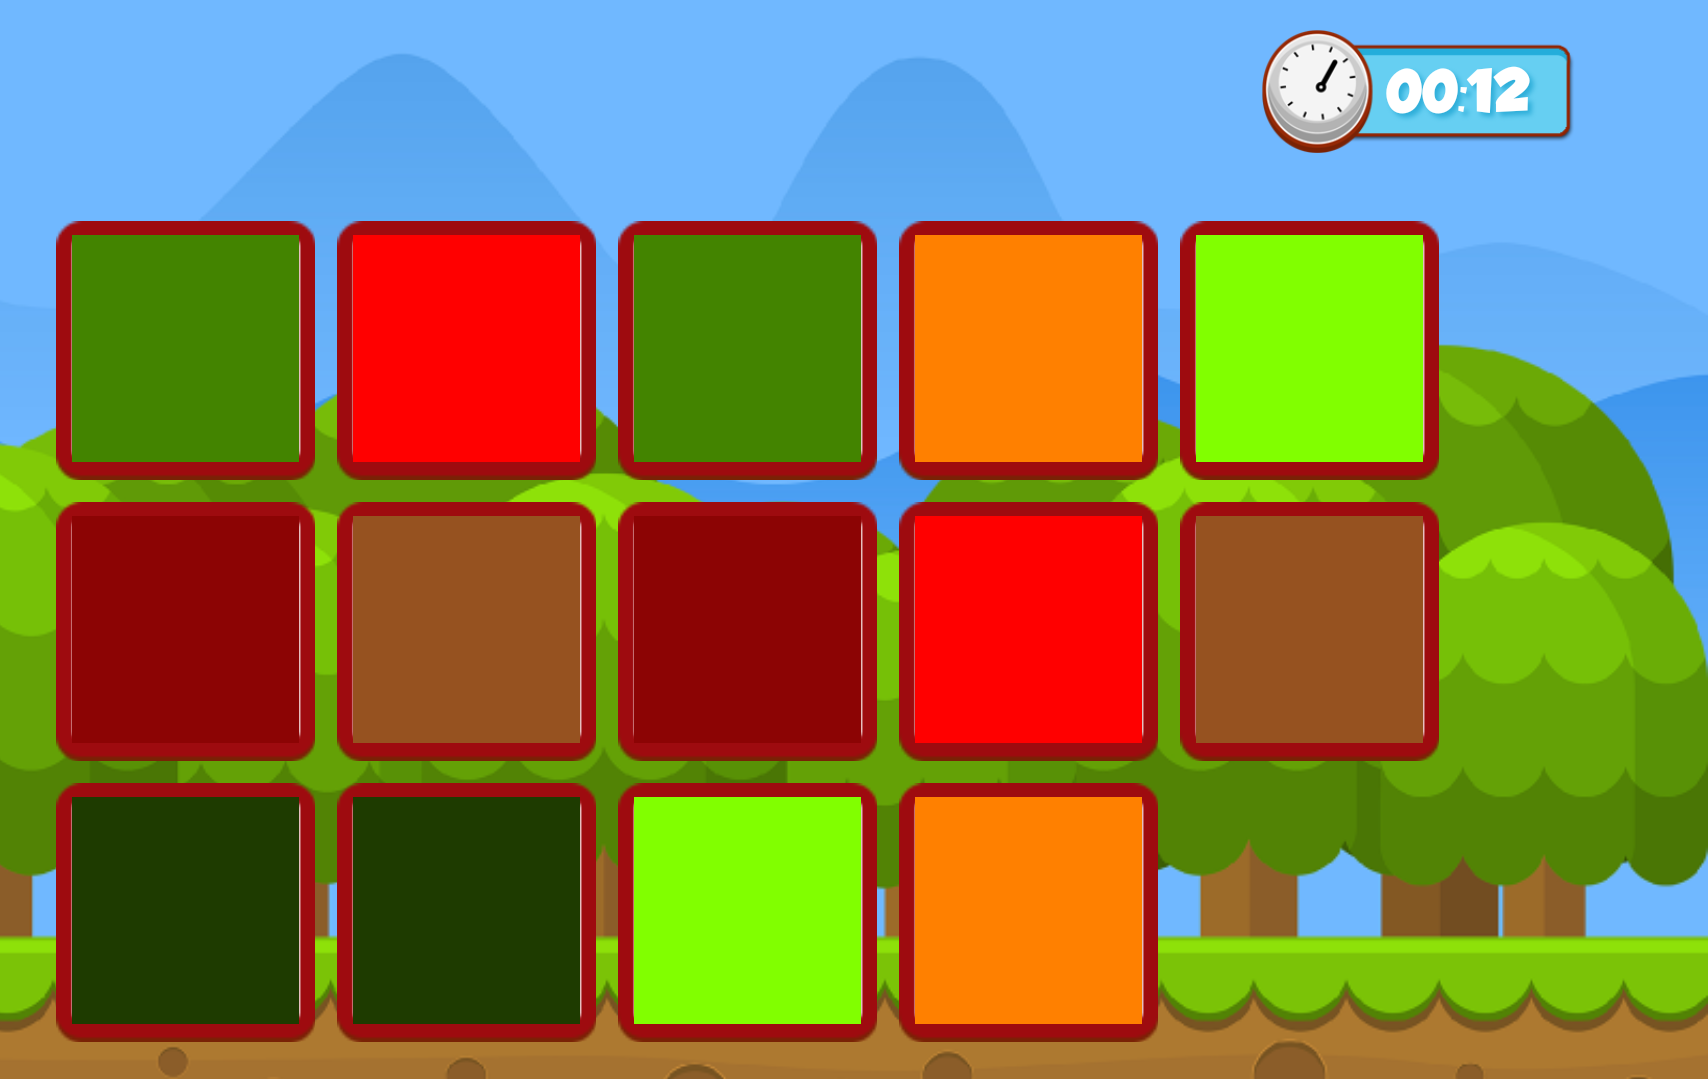
\includegraphics[width=13.5cm]{images/noObstTurned.png}
	\caption[Screenshot of the game without any obstacles.]{Screenshot of the game without any obstacles. All cards are turned face up.}
	\label{fig:noObstacle}
\end{figure}

\begin{figure}[H]
	\centering
	
\includegraphics[width=13.5cm]{images/glareEffect.png}
	\caption[Screenshot of the game field with simulated sunlight.]{Screenshot of the game field with simulated sunlight. Sunbeams are especially visible on the right hand side. All cards are turned face up.}
	\label{fig:glareEffect}
\end{figure}
\chapter{Collected Data}
\label{collected_data}
While the subjects played the memory game, behavioural data and brain activity data was collected. Relevant for this work is only the behavioural data recorded in glare effect and no obstacle games.
The eeg data is not used, because the aim is to exploit behavioural patterns of natural HCI situations without using any additional sensors. %Detecting interaction obstacles using only the behavioural data has also been done The same approach  like it has been done before for memory obstacles. \cite{salous_putze_2018esann}. Instead only behavioural data is used, that can be collected without being noticed by the user.
Therefore, eeg data will not be further explained. The data was collected from 22 subjects. They were university students between the age of 18 and 28. Each subject except one recorded two no obstacle and one glare effect game. The one exception did not record any glare effect games. As a result, there are 44 no obstacle and 21 glare effect games. The data was already provided and was not collected during this bachelor thesis.

%\section{Behavioural data}
%\label{behavioural_data}

\begin{minipage}[b]{0.6\textwidth}
	In order to record behavioural data, each of the 14 cards was initially given a fixed card code and is was recorded which pairs of cards were turned face up in each round. The card code consists of two numbers separated by a dot. The first number specifies the colour of the card (between 1 and 7 as there are 7 colours) and the second number specifies if it is the first or second card with that colour. Once a game is started, all cards are shuffled. The initial assignment of colours to numbers between 1 and 7 is shown in table \ref{tab:colorAssign}.
\end{minipage}
\begin{minipage}[b]{0.4\textwidth}
	
	\begin{table}[H]
		\centering
		
		\begin{tabular}{|c|c|}
			\hline
			Colour & Number  \\
			\hline
			Dark green & 1 \\
			Brown & 2 \\
			Red & 3 \\
			Light green & 4 \\
			Green & 5 \\
			Orange & 6 \\
			Dark red & 7 \\
			\hline
		\end{tabular}
		\caption[Static assignment of colours to numbers]{Static assignment\\\hspace{0\textwidth}of colours to numbers}
		\label{tab:colorAssign}
	\end{table}
\end{minipage}




The behavioural data was saved in logs, consisting of the card codes of each round followed by the timestamps of when the cards were flipped. Data of 20 rounds and therefore at maximum 40 flipped cards was recorded. If the game was completed in less than 20 turns, the remaining card code entries were filled with 0.0 and the remaining timestamp entries were filled with 0. An example of the sequence of card codes recorded during a game can be seen in the top half of table \ref{tab:mappings}. The timestamps are irrelevant for this work and therefore not shown. 

\begin{minipage}{0.5\textwidth}
	With the assignments shown in table \ref{tab:colorAssign}, the first card code in the upper sequence of table \ref{tab:mappings} means that the first card to be flipped was the second green card. In the same turn, the second card that was turned around was the second brown card. This mapping is static as colours have the same numbers across all recorded games. However, the simulator requires a dynamic mapping of the card codes. By dynamic mapping of the card codes is meant, that the colours are not assigned to fixed numbers but that the numbers are assigned in the reveal order specific to each game. This becomes clear, by looking the card code sequence from above, but dynamically mapped. This can be seen in the bottom half of table \ref{tab:mappings}. 
\end{minipage}
\begin{minipage}{0.5\textwidth}
	
	\begin{table}[H]
		\centering
		
		\begin{tabular}{|c|}
			\hline
			\\
			Static mapping:  \\
			5.2,2.2,4.2,4.1,6.1,7.2,6.2,6.1,1.2,1.1,\\
			7.1,2.2,2.1,7.1,5.2,5.1,3.1,2.1,7.1,3.1,\\
			7.2,7.1,3.2,2.2,2.1,2.2,3.1,3.2,0.0,0.0,\\
			0.0,0.0,0.0,0.0,0.0,0.0,0.0,0.0,0.0,0.0 \\
			\\
			\hline
			\\
			Dynamic mapping: \\
			1.1,2.1,3.1,3.2,4.1,5.1,4.2,4.1,6.1,6.2,\\
			5.2,2.1,2.2,5.2,1.1,1.2,7.1,2.2,5.2,7.1,\\
			5.1,5.2,7.2,2.1,2.2,2.1,7.1,7.2,0.0,0.0,\\
			0.0,0.0,0.0,0.0,0.0,0.0,0.0,0.0,0.0,0.0 \\
			\\
			\hline
		\end{tabular}
		\caption[Static and dynamic mapping of card codes.]{Static and dynamic\\\hspace{0\textwidth}mapping of card codes}
		\label{tab:mappings}
	\end{table}
	
	%\begin{center}
	%	Static mapping:\\
	%	5.2,2.2,4.2,4.1,6.1,7.2,6.2,6.1,1.2,1.1,\\
	%	7.1,2.2,2.1,7.1,5.2,5.1,3.1,2.1,7.1,3.1,\\
	%	7.2,7.1,3.2,2.2,2.1,2.2,3.1,3.2,0.0,0.0,\\
	%	0.0,0.0,0.0,0.0,0.0,0.0,0.0,0.0,0.0,0.0
		
		
	%	\begin{center}
	%		Dynamic mapping:\\
	%		1.1,2.1,3.1,3.2,4.1,5.1,4.2,4.1,6.1,6.2,\\
	%		5.2,2.1,2.2,5.2,1.1,1.2,7.1,2.2,5.2,7.1,\\
	%		5.1,5.2,7.2,2.1,2.2,2.1,7.1,7.2,0.0,0.0,\\
	%		0.0,0.0,0.0,0.0,0.0,0.0,0.0,0.0,0.0,0.0
	%	\end{center}
	%\end{center}
\end{minipage}


In this dynamic mapping of the card codes, each entry likewise consists of two numbers that are separated by a dot. However, the numbers are differently interpreted. The first number specifies what number of colour it is to be revealed and the second number specifies if it was the first or the second card of that colour. In the example above the colour green is the first to be revealed and therefore assigned to the value 1. As it is the first green card revealed the second component of the card code is 1 as well. As a result, the first entry is 1.1. Then a brown card is turned face up, meaning the second entry is 2.1 since it was the first brown card. Once the other brown card is discovered, the entry for that step will be 2.2. This pattern continues throughout the whole sequence. This means that the mapping is specific to each game and depends on the reveal order of the cards. These card codes are the foundation for the features calculated in section \ref{feature_generation} \nameref{feature_generation}.

%Additionally similarity values for each card code are added to the logs. These values are meant to describe how the colour difference of the two cards described by that card code are perceived by the human eye. These similarity values are initially just placeholders, as a similarity matrix for the glare effect has not been created, yet. Furthermore these values are only rele

%\todo{umschreiebne!}
%Additionally the logs are extended with a each of the dynamically mapped card codes receives a similarity value, provided by a similarity matrix. Each card codes describes the two cards that were flipped in a turn and the similarity value describes how similar the colours of the two cards are. These similarity assignments are relevant  for each combination of colours needed to be added to the logs. The assignments had to be made according to the dynamic mapping of card codes. The similarity values are extracted from a similarity matrix.
%As mentioned above the similarity values for the card codes must also be dynamic.  The differnece bewteen static and dynamic similarity assignments is explained in section \todo{ref zu similarity matrix bei simulator und da erklären was die unterschiede sind und was der simulator benutzt? genauso köönte man dann aber auch die card codes mapping da erklären?}

Logs with remapped card codes were already provided, but an additional component in the glare effect logs is needed in order to successfully simulate new games. The logs are used in the simulator to generate new games. When simulating the glare effect, the simulator requires a similarity matrix, that that correctly describes the colour differences of the cards under the influence of the glare effect, which does not exist yet. The creation of this matrix is done in section \ref{similarity_matrix_cretion} \nameref{similarity_matrix_cretion} and its values are added to the glare effect logs in section \ref{incorporation_of_the_new_similarity_matrix} \nameref{incorporation_of_the_new_similarity_matrix}. Contrary to the glare effect logs, in the no obstacle logs, no changes need to be made, as the simulator does not use any similarity values when simulating no obstacle games. It should also be noted that the provided logs with remapped card codes additionally include four statistical features for the last turn. These consist of the number of remaining cards, the number of never revealed cards, the highest number of times the same card was revealed and the number of rounds since all pairs were found. These four values are ignored, as they are newly calculated for every step as explained in section \ref{1d_cnn_features} \nameref{1d_cnn_features}. Last but not least all logs end with a label, describing in which game mode the log was created. 

%there was a change to be made regarding the glare effect logs before they could be used. The similarity matrix for the glare effect game was just a placehoulder and did not correclty portray the color differneces under the influence of sunlight. To successfully simulate glare effect games the simulator requires such an similarity matrix. Therefore a new one is created in section \todo{ref}. The old similarity values in the glare effect logs are then replaced with the new values in section \todo{ref}. Contrary to the glare effect logs, in the no obstacle logs, no changes need to be made, as the simulator does not use any similarity values when simulating no obstacle games. It should also be noted that the provided logs with remapped card codes additionally include four statistical features for the last turn. These consist of the number of remaining cards, the number of never revealed cards, the highest number of times the same card was revealed and the number of rounds since all pairs were found. These four values are ignored, as they are newly calculated for every turn in section \todo{ref}. Last but not least all logs end with a label, describing in which game mode the log was created. 

%Logs with remapped card codes and added similarity values were already provided, but there was a change to be made regarding the glare effect logs before they could be used. The similarity matrix for the glare effect game was just a placehoulder and did not correclty portray the color differneces under the influence of sunlight. To successfully simulate glare effect games the simulator requires such an similarity matrix. Therefore a new one is created in section \todo{ref}. The old similarity values in the glare effect logs are then replaced with the new values in section \todo{ref}. Contrary to the glare effect logs, in the no obstacle logs, no changes need to be made, as the simulator does not use any similarity values when simulating no obstacle games. It should also be noted that the provided logs with remapped card codes additionally include four statistical features for the last turn. These consist of the number of remaining cards, the number of never revealed cards, the highest number of times the same card was revealed and the number of rounds since all pairs were found. These four values are ignored, as they are newly calculated for every turn in section \todo{ref}. Last but not least all logs end with a label, describing in which game mode the log was created. 

%The other neccessary change derived from the fact that although the card codes were dynamically mapped, the similarity assignments were made according to the static mapping of the card codes inestead of the dynamic mapping. This meant that the assignment of simialrity values to numbers for the cards compared were identical in all games, but the numbers of the cards stood for different colours in different games. To solve this issue the newly created similarity matrix for the glare effect was used to determine the dynamically mapped similarity values for each game.



%\section{Brain activity}
%\label{brain_activity}
%\todo{das weg und stattdessen einfach oben als begründung kurz rein. dann hat man auch weniger sections und 2 seiten weniger}
%Eeg data collected from all proabnds during the game. However, there is one problem with using the eeg data: The overlyiong context of this work is to find interaction obstacles and ultimatley imporve the user interaction. This means that the way of discovering such an interaction obstacle should not worsen the interaction experience. If all people had to waer eeg masks when interacting with software for the purpose of detecting interaction obstacles, the interaction experience itself would suffer. A method of recording brain activity without an deterioration of the interaction experience has not been discovered yet. Additionally it is not cost efficient for every user to use and eeg sensor. As a result the decision was made not to use eeg data and instead only use the behvioural data that is collected direclty through the interaction and stays unnoticed by the user. As eeg data is not used in this work it will not be further explained. 



\chapter{CMM-based Cognitive User Simulation}
The cognitive system lab developed the computer program cognitive memory model (CMM).
It utilizes concepts of the act-r-theory to model the cognitive human memory. ACT-R is a cognitive architecture that aims to describe and integrate  central basic mechanisms of human cognition. \todo{ref:  \url{https://www.google.com/search?q=intimates+deutsch&oq=iminates+&aqs=chrome.1.69i57j0l7.2543j0j15&sourceid=chrome&ie=UTF-8}} In the context of the matching pairs game the CMM was used to implement a generative model. By modelling memorized and forgotten revealed cards and deciding in each turn whether to explore unknown cards or to exploit the gathered knowledge to reveal matching pairs, the course of a matching pairs game can be simulated taking the capability of human memory into account. Furthermore it is possible to define a similarity matrix to simulate similarities between cards in matching pairs games. This matrix includes similarity values for each colour combination of cards. Such a similarity matrix can be used in the context of visual interaction obstacles to emulate human confusion. In related research it was used to simulate the confusion caused by colour blindness and the usage of a red-green card set. For this thesis the only two modes that are relevant are the glare effect (no assistance) and the no obstacle (no assistance) modes. In order to simualte no obstacle games no simialrity matrix is needed, but for glare effect games a new similarity matrix is created in section \todo{ref}.



%- to capture the differnce between colours in the way humans observe it, the rgb scale is not suitable... grund. Therefore cie is usd
%- was wichtig für diese arbeit ist: no óbsracel un glare 
%- für no obstacle hat die wird keine similarity matrix verwendet. (bzw. werte der matrix so gewählt dass sie keinen einfluss haben)
%- für glare effect muss eine neue definiertt werden wie in chapter ref
%- so wie ich es gemacht habe mit den werten
%- as metioned formerly the cie1976 is used. es gibt ein neues dass die unterschiede realistis her darstellt cie2000. deshalbw ird das stattdesen benutzt bei erstellung der matrix für glare effect

To accurately simulate the performance of human memory multiple parameters are randomly initialized and then repetedly optimized using a genetic optimization algorithm. These parameters can be further extended. The genetic algorithm works by repeadily simulating game sessions and updating the parameters by applying mutation and selection operations. To select the best parameter values two performance measurements are defined and used to compare the simulated game sessions and a real game as reference. These perfomarmce measurements are the number of matching pairs and the number of penalties per round. Penalties are given if a card is revealed whose partner has already been seen before but the pair was not picked up. The optimization of the parameter population is repeated over many generations so that the performance in the simalted games best fits that in the real game. As example one of the paramameters optimimzed by the genetic optimization algorithm is the similarity decay. It reduces the similarity effects during the course of the game, since the user may learn to adapt to the visual interaction obstacle and therefore be less effected by it. Furthermore the similarity effect is continuelasly reduced as there are less cards in the game after pairs were discovered. 

As input the simulator takes a number of game logs and simulated a specified amount of new sessions using the genetic optimization algorithm. For instance 20 game logs can be passed to simulate 1000 new sessions out of each game log, resulting in 20000 simulated games. The data contained in the game logs is shown in section \todo{ref}. In the context of simulating no obstacle games improvements to the simulator were made that are explained in section \todo{ref}. 

%\section{Similarity Matrix}
%- auch erklären was similarity matrix ist, struktur und wie die benutz wird\\
%- and colour representation cie etc delta e color differnece, vs rgb was das bringt\\ 
%- no special similarity matrxi for noosbst needed. The differneces can simply be calculated. it is already used in the simulator. However a new similarity matrix needs to be created for simulating glare effect games. 
%- für no obst wird identity similariity matrix verwendet: diagonale ist 
\chapter{Data Preparation}
\label{data_preparation}
%\begin{figure}[H]
%	\centering
%	\begin{tikzpicture}[node distance = 4cm, auto]
%	% Place nodes
%	\node [block] (matrix) {Create similarity matrix for glare effect};
%	\node [block, right of=matrix, node distance=5cm] (mapping) {Mapping};
%	\node [block, right of=mapping, node distance=5cm] (valid) {Valid logs collection};
%	\node [block, below of=matrix] (quality) {quality plotting};
%	\node [block, below of=mapping] (sorting) {Sorting of logs};
%	\node [block, below of=valid] (simulate) {Simulation};
%	\node [decision, below of=quality, node distance=4cm] (decide) {Are simulated logs realistic?};
%	\node [block, below of=simulate] (change) {Change simulator};
%	\node [block, below of=decide] (generate) {Generate features};
%	\node [block, below of=change] (train) {Proceed with traning};
%	
%	% Draw edges
%	\path [line] (matrix) -- (mapping);
%	\path [line] (mapping) -- (valid);
%	\path [line] (valid) -- (simulate);
%	\path [line] (simulate) -- (sorting);
%	\path [line] (quality) -- (decide);
%	\path [line] (sorting) -- (quality);
%	\path [line, pos=0.12] (decide) -- node {No}(change);
%	\path [line] (change) -- (simulate);
%	\path [line] (decide) -- node [midway] {Yes}(generate);
%	\path [line] (generate) -- (train);
%	
%	\end{tikzpicture}
%	\caption[Bild kurz]{hi}
%\end{figure}
To prepare the data for the training many steps were neccesary. One big step is to increse the available dta by simulaing user behaviour. Therefore the simulator	tor in chapter \todo{ref} is used. For simulating games with no opbstacle there is no need for a similarity matrix. However, in order to sucessfully simulate glare effect games, a special similarity matrix is required. While without any obstacles the color differnes are independent from the position of the crads, this is not the case in glare effect games since the intensity of the light is not the same across the whole field. As a result the first step is to create a similarity matrix that descirbes the differneces of colours under the influence of the glare effect. Once completed, it replaces the old similarity matrix in the glare effect logs. As not all logs are valid and can be used in the simulator, the invalid log must be removed. These valid logs are then used to simulate user behaviour and thereby create new logs. These simulated logs are sorted by their quality and the simualtion is evaluateed. If the performance in the simulated games is similar to that in the original games it is preceeded with the gerneration of the features for the training. Otherwise changes to the simulator ar made and the simulation, the sorting and the evaluation are repeated. In case of very bad simulations of glare effcet logs it would have also been possible to change the approch of creating the similarity matrix or find a new approch. However, the simualtinos of glare effect were very good, which can be seen in \todo{ref}, which is why the spproach was kept.

\section{Similarity matrix creation}
\label{similarity_matrix_cretion}

%\section{Glare effect similarity matrix}
%\subsection{Matrix generation}
\subsection{Conceptualization}
\label{conceptualization}
The aim is to create a similarity matrix that descibes the differneces between colours under the influence of the simulated sun light. The difficulty hereby is that the intensity of the light is not spread evenly across the whole field. Instead, as it would be if a real sun would shine onto the display, a certain are has the highest intensity and the intensity is lower the further away from that area. Adittionally there are wide lines of higher intensity comming from the brightest area, that simulate sunbeams. This influence of the simulated sunlight can be seen in figute \ref{fig:glareEffect}. 

\begin{figure}[H]
	\centering
	
\includegraphics[width=14cm]{images/glareEffect.png}
	\caption[Bild kurz]{Screenshot of the game field with simulated sunlight. Sunbeams are especially visible on the right hand side. All cards are turned face up.}
	\label{fig:glareEffect}
\end{figure}
\todo{vielleicht bild raus nehmen weil es oben schon einmal ist und referenzien nach oben}

As a result simply extracting the rgb values for one pixel of each card in one game and calculating the differneces has two major problems: Firstly, the differences are highly influenced by the position of the specific cards. If the matrix is calculated using a single glare effect game the differneces are only representative for exactly that game and may be completely differnet if the cards are positioned differently. Secondly, extracting single pixels for each card in an image could lead to color values that do not represent the overall observed colour due to varying brightnesses on differnet points of a card. This behaviour is undesired, as the final similarity matrix is supposed to represent the differneces of the observed colours of the cards. \todo{vielleicht quelle suchen die sagt das menschen farbenm ion bereichen mitteln oder so} In order to solve these problems a more complex approach then simply extracting single pixels out of a game was needed. 

The problem of the positional influence can be solved by creating similarity matrices for more than one game and calculating the mean color differences of those matrices. The idea is that by creating using so many games that all or most combinations of positions and colours are included and calculating the mean of all comparissons for , the result will not be influenced by the position of the cards.  However, first needs to be determined which number of games satisfies this condition. Each game consists of 14 cards, with each two cards having the same colours. When determining the difference between two colours there are two differnet cases: 
\begin{itemize}
	\item 1. The colours are not the same: In each game there are exactly 4 combinations of positions for those two colours, because there are two cards for each colour. 
	\item 2. The colours are the same: In each game there is only one combination of positions for those colours.  
\end{itemize}

\begin{figure}[H]
	\centering
	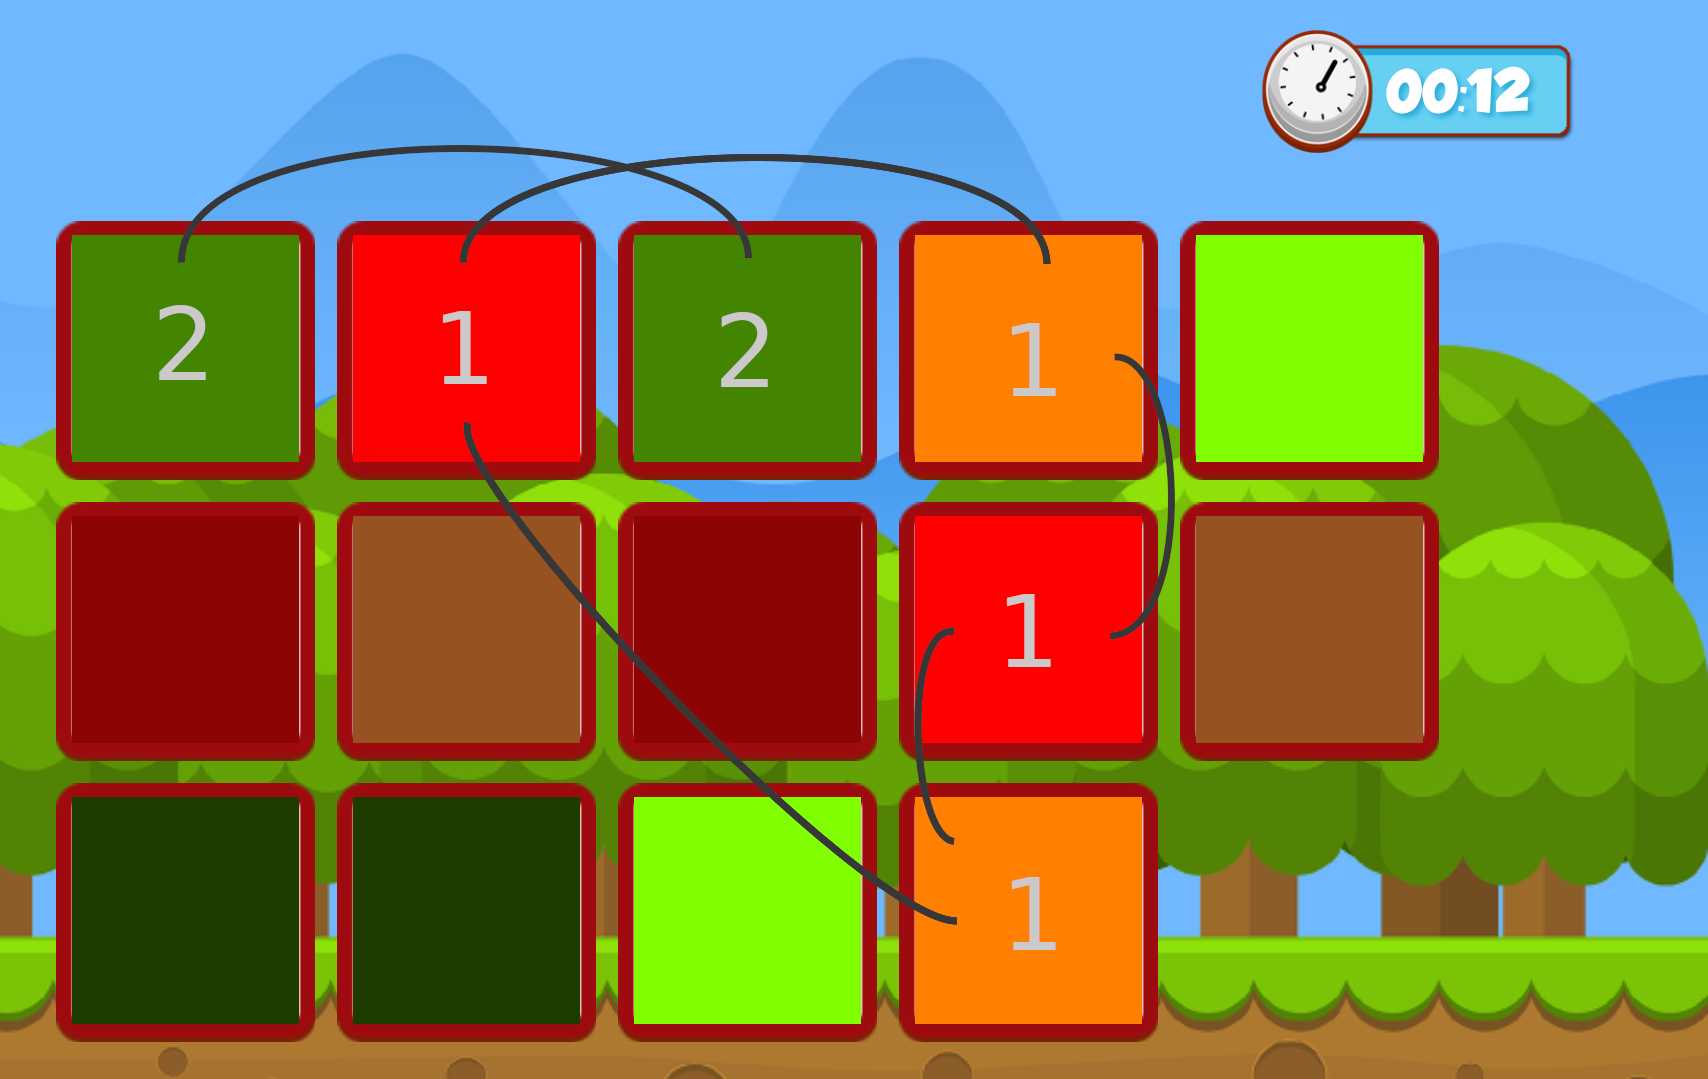
\includegraphics[width=14cm]{images/noObstTurnedNotes.png}
	\caption[Bild kurz]{Examplary showing the number of different comparissons for case 1 and 2. The numbers on the cards represent the case and the edges indicate unique comparissons. All cards are turned face up. A game without any obstacles is used only for the purpose of clarifying the differnet comparissons. All screenshots used for the actual calculation are taken from glare effect games.}
	\label{fig:noObstTurnedNotes}
\end{figure}

First it is calculated how many screenshots are necessary for the first case. For two different coloured arbitrary but fixed cards there can be 
\begin{equation*}
C\textsubscript{1} = 14 \cdot 13 = 182 
\end{equation*}
combinations of positions are possible. The reason that it is not not 14 $\cdot$ 14 is that 14 comparissons of cards with themself would be included. We formulate the condition that enough screenshots need to be taken so that a arbitrary but fixed combination of positions for two different colours is included with a probability of 95\%. 

\begin{center}
	As there are 4 such combinations of positions in each game the probanility P(A) to get a specific combination in a game is 
	\begin{equation*}
	P(A) = \frac{4}{182} % = 0.02198
	\end{equation*}
	The counter probability P($\lnot$A) is 
	\begin{equation*}
	P(\lnot A) = 1 - \frac{4}{182} = \frac{178}{182}%0.02198 = 0.97802
	\end{equation*}
	The number of necceary screenshots to include a specific combination with 95\% probaility is calculated by solving
	\begin{align*}
	1 - P(\lnot A)^n &\geq 0.95 \\
	1 - \left(\frac{178}{182}\right)^n &\geq 0.95 \\
	1 &\geq 0.95 + \left(\frac{178}{182}\right)^n\\
	\left(\frac{178}{182}\right)^n &\leq 0.05\\
	n &\geq log_{(\frac{178}{182})}(0.05) \\
	n &\geq 134.8024 %\llap{$\implies$\hspace{50pt}} at beginnging for implication arrow
	\end{align*}
\end{center}
This means that about 135 Screenshots of games are needed in the first case. Now we perform the same calculation for the second case where there is only one combination of positions for the colours. However, there are less combinations of positions that are relevant than in the first case. For example for two green cards at index 0 and 1 the 182 comparissons would include a comparison of the first green card and the second green card as well as a comparisson of the second green card and the first green card. This goes for every two cards with the same colour, meaning there are only half as many different comparissons in the second case than in the first case. As a result the number of possible combinations in the second case is
\begin{equation*}
C\textsubscript{2} = \frac{C\textsubscript{1}}{2} = \frac{14 \cdot 13}{2} = 91.
\end{equation*}
Now we calculate how many screenshots must be taken to include a specific combination of positions for two equal colours with a probability of 95\%. 
\begin{center}
	As there is one such combinations of positions in each game the probanility P(A) to get a specific combination in a game is 
	\begin{equation*}
	P(A) = \frac{1}{91} % = 0.02198
	\end{equation*}
	The counter probability P($\lnot$A) is 
	\begin{equation*}
	P(\lnot A) = 1 - \frac{1}{91} = \frac{90}{91}.%0.02198 = 0.97802
	\end{equation*}
	The number of necceary screenshots to include a specific combination with 95\% probaility is calculated by solving
	\begin{align*}
	1 - P(\lnot A)^n &\geq 0.95 \\
	1 - \left(\frac{90}{91}\right)^n &\geq 0.95 \\
	1 &\geq 0.95 + \left(\frac{90}{91}\right)^n\\
	\left(\frac{90}{91}\right)^n &\leq 0.05\\
	n &\geq log_{(\frac{90}{91})}(0.05) \\
	n &\geq 271.111 %\llap{$\implies$\hspace{50pt}} at beginnging for implication arrow
	\end{align*}
\end{center}
This means that about 272 screenshots of games are needed in the second case. As there are more screenshots needed for the second case, the first case is also included. This inclusion is caused by the fact that each screenshot includes comparissons for the  fist  as well as the second case. To have a buffer the decision was made to take screenshots of 300 games. In theory these screenshot include any arbitrary but fixed combinations of positions and colours with a probability of over 95\%, which should eliminate the problem of the positional influence.

Nonetheless, this does not solve the second problem of extracting single pixels that can potentially be directly in the area of a sunbeam. This can be fixed, by extracting all pixels in a certain are of the card and averaging their rgb values.  %By averaging all colours in a certain area, the result will be more representitive of what the player actually sees \todo{Quelle finden wo sowas über visuellen kram gesagt wird}. 

Last but not least it needs to be clarified how the colour differneces are calculated. To capture how colour differences are observed by humans, the rgb colour scale is not suitable. Using the rgb colour scale simirlarly stromng perseaved color differnces do not neccessarily have the same eucliidean distance. Contrary to that the CIELAB colour space aims to do exaclty that. Although not perfect, it more accurately descirbes human colour perception than the rgb colour space. Therefore the colour differences described in the similarity matrix are calculated after converting the colours into the CIELAB colour space. The colour distance is called Delta E score. The lower this score is the more similar appear the colours to human eyes. In related work, when creating the similarity matrix for the effect of colour blindness, the CIE1976 colour model was used for the calculations. However, the formula for calculating the colour difference has since then been improved multiple times, resulting in the CIE2000 colour model. Through multiple modifications of the formula it got closer to a visual equidistance, meaning simirlarly stromng perseaved color differnces have more similar Delta E scores than before. Therefore when creating the similarity matrix for the glare effect the CIE2000 colour model is used instead of the old one. 

To sum it up, the chosen approach is to take 300 screenshots of glare effect games with all cards turned face up, extracting areas of rgb values for each card, converting the average rgb values of ares into CIELAB colours, calculating a similarity matrix for each game that contains the delta E scores and finally averaging the delta E scores across all similarity matrices. To achieve values between 0 and 1, the colour differneces additionally need to be scaled down in the end.
 
\subsection{Screenshot extraction}
\label{screenshot_extraction}
To play the memory game and take screenshots an emulator for the pixel 2 in android studio was used. In order to take the screenshots in the needed way and collect additionally necessary information some changes to the memory game were made. In the way the game is intended there are always only maximum two cards turned face up. However, for the screenshots all cards need to be turned around so that the colour differneces can be calculated. Therefore the memory game was adjusted so that all cards are turned face up once the player turns a card. Additionally it was changed so that cards stay face up once they get turned around for the first time. This makes it possible to take screenshots with the colours of all cards visible. Furthermore, for the creation of the similarity matrix it needs to be known what the original colours without the influnece of the simulated sun are. To collect the screenshots and the according colours of the cards in each game a semi-automatic approach was chosen. Once a game is started and a card is flipped, resulting in all cards being turned face up, the colours of all cards are saved in a list. Then a screenshot is manually taken and afterwards the game is exited to enter the main menu. From there on the process is repeated 300 times. As a result there are 300 hundred screenshots of games and a two dimensional list that includes the colours of the cards in the 300 games. The first dimension specifies the game and the second dimension the index of the card. The values of this list are stored in a text file before the game is completely closed. To assure that no mistakes were made when taking the screenshots, the number of collected screenshots is observed during the whole process and afterwards all screenshots are manually checked so that all cards are turned face up.

\subsection{Implementation}
\label{implementation}
This section will show and explain the implementation of the similarity matrix generation. Code is only included if it helps to further understand what is being explained. First of all the screenshots and the information about the original colours of the cards are loaded. Before the actual calculation of a similarity matrix for each image, the average rgb values of the cards on the field need to be determined. 

\begin{lstlisting}[language=python, caption=Add caption, xleftmargin=5.0ex]
def determine_glare_rgb_values(image):
'''
Calculates the rgb average rbg values for each card in an image.
:param image: The screenshot of the memory game with all cards 
turned face up.
:return: The average rbg values in the specified 150 x 150 pixel 
areas for each card. 
'''
glare_rgb_values = []
for corner in card_corners:
	x_border = corner[0] + 150
	y_border = corner[1] + 150
	card_values = []
	for x in range(corner[0], x_border, 1):
		for y in range(corner[1], y_border, 1):
			coordinates = x, y
			pixel_values = image.getpixel(coordinates)
			card_values.append(pixel_values[:-1])
	card_r = int(round(np.mean([color[0] for color in card_values])))
	card_g = int(round(np.mean([color[1] for color in card_values])))
	card_b = int(round(np.mean([color[2] for color in card_values])))
	glare_rgb_values.append((card_r, card_g, card_b))
return glare_rgb_values 
\end{lstlisting}
The cards are each 250 $\cdot$ 250 pixels big and the rgb values are extracted from squared 150 $\cdot$ 150 pixel areas. The coordinates the pixels are extracted from are manually selected in gimp. As a result the areas are only correct for the used resolution of 1080p. Once the mean rgb values in those areas are calculated and converted into LAB colours the similarity matrix can be created. LAB colours are neccessary to calculate the colour differnece using the CIE2000 colour model. Each of the 28 cells in the similarity matrix falls into one of the two cases explained in \todo{ref}, meaning there are either 4 or only 1 unique combination for the calculation of each cell value. For every combination the lab colour distance is determined and the values for each cell are averaged. This completes the steps for a single image, resulting in a similarity matrix with unscaled values. 
%\begin{lstlisting}[language=python, caption=Add caption]
%def determine_distance(color_1_rgb, color_2_rgb):
%	'''
%	Determines dinstance between colors with delta e formula. 
%	:param color_1_rgb: The first color.
%	:param color_2_rgb: The second color.
%	:return: The delta_e distance between the two colours. 
%	'''
%	lab_1 = convert_color(color_1_rgb, LabColor)
%	lab_2 = convert_color(color_2_rgb, LabColor)
%	
%	if cie_1976:
%		detlta_e = delta_e_cie1976(lab_1, lab_2)
%	else:
%		detlta_e = delta_e_cie2000(lab_1, lab_2, Kl=1, Kc=1, Kh=1)
%	return detlta_e
%\end{lstlisting}
Once a similarity matrix with unscaled values for every image is created, the average of all matrices is calculated. During the whole calculation of the single matrices it is being kept track of the highest occurring colour differnece. The last step neccessary to complete the final similarity matrix is to divide all values in the matrix by use the highest colour differnce to scale them down to be between 0 and 1. 

%Through the original colours loaded in the beginning, the coverage of combinations in the 300 games can be calculated. 
%\begin{lstlisting}[language=python, caption=Add caption]
%def determine_coverage(original_colors):
%'''
%For calculating how many of the combinations are includes 
%in the calcuation. 
%The calculations are based on having 14 cards on the field.
%:param original_colors: A list containing tuples with the card name, 
%the mappimg number for the card, and the index for each card on the 
%screenshot for all screenshots.
%:return: The coverage of combinations of positions 
%for all colour combinations. 
%'''|\Suppressnumber|

%[...]|\Reactivatenumber{18}|

%combinations = []
%for colors in original_colors:
%for i in range(len(colors)):
%original_color_1 = colors[i]
%for l in range(len(colors)):
%original_color_2 = colors[l]
%if original_color_1[2] != original_color_2[2] and (original_color_2, original_color_1) %not in combinations and (original_color_1, original_color_2) not in combinations:
%combinations.append((original_color_1, original_color_2))    
%return len(combinations) / number_of_total_combinations
%\end{lstlisting}

\subsection{Testing}
\label{testing}
To verify the correcteness of the color extraction and the calculation of the similarity matrix, the main funtionalities are manually tested. The colour extraction was tested by extracting colours of a screenshot with the skript and compoaring the rgb values to the actual values in the images using gimp. Furthermore the calculation of the delta e score was tested, by comaring results of the script with those of an online calculator. \\

To assure that the 300 games actually include most of the combinations and therefore eliminate the positional influence of cards, the coverage of combinations can be additionally calculated. Therefore the number of unique combinations included in the 300 screenshots must be divided by the overall number of possible combinations. The number of unique combinations can be counted during the process of creating the similarity matrix, but the number of possible combinations must seperatly be determined. The similarity matrix for glare effect has 28 entries, from which 7 are comparissons between same and 21 between different colours. With \textit{C\textsubscript{1}} and \textit{C\textsubscript{2}}  being the possible combinations for two arbitrayry but fixed coloured cards in the two cases mentioned above, the number of overall possible combinations C is
\begin{align*}
	C &= 21 \cdot C\textsubscript{1} + 7 \cdot C\textsubscript{2}\\
	&= 21 \cdot 182 + 7 \cdot 91\\
	&= 4459. 
\end{align*}
The 300 games used for creating this matrix include 99.57\% of all possible combinations. Furthermore is was verified that certain combinations are not included significantly more often than others and in that sense have stronger influence on the result. \todo{code ergänzen und nachprüfen wie oft die combinationen vorkamen..histogramm?}. 

\subsection{Final Matrix}
\label{final_matrix}
In figure \ref{fig:simMatrix} the final similarity matrix can be seen, dsiplaying how colour differneces are observed under the influence of the simulated sunlight, averaged over 300 games. As mentioned before, the lower the delta e score the more similar the cards appear to the human eye. The maximum delta E score that occured during the calculation was 8.861. All values are divided by that number to achieve scores between 0 and 1.
%maximum distance: 8.861003756554735.
\begin{figure}[H]
	\centering
	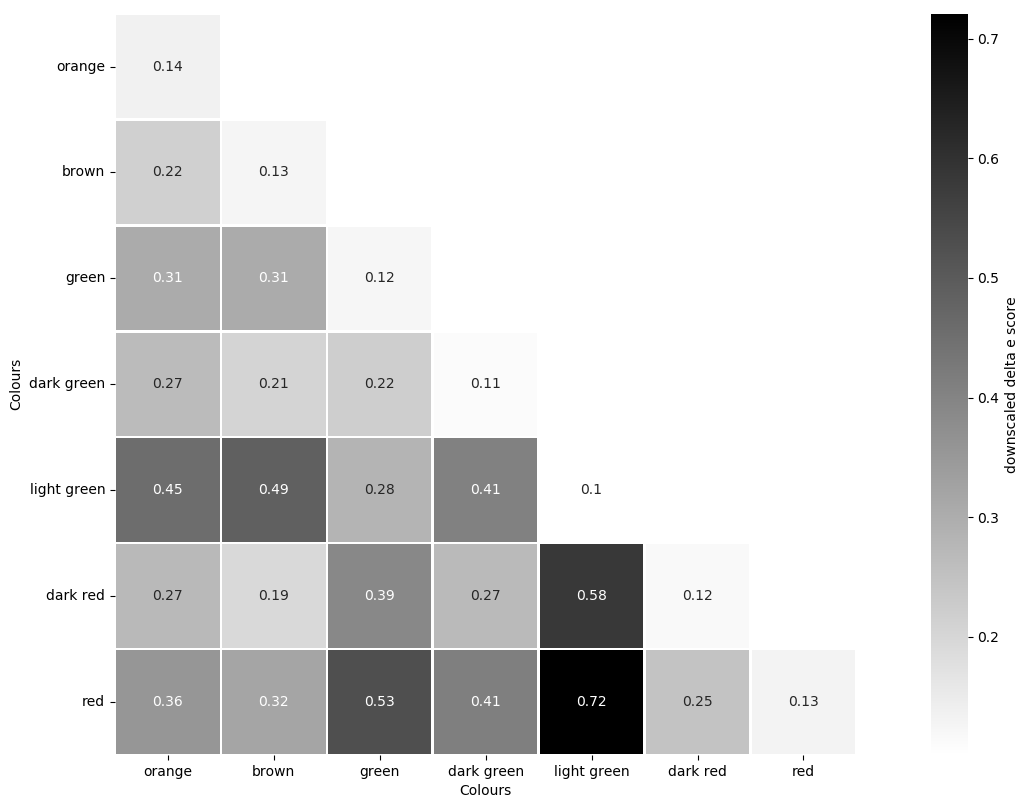
\includegraphics[width=15cm]{images/simMatrixGrey.png}
	\caption[Bild kurz]{Add caption. The lighter the colour the less a difference is noticeable}
	\label{fig:simMatrix}
\end{figure}
The delta E score is less a definitive answer, and instead a helpflu metric to apply to a specific use case. Although there are tendencies regarding the interpretation of colour differences, there is no definitive table that descriebes what the different scores mean. One reason for this is that the perceived colour differnece may vary in different situations and circumstances. For instance, is the colour difference perceived differently depending on how long the colours are exposed to the human eye, as humans can over time adapt to the colours. This means that in a setup where all colours are always visible the colour difference will likely be perceived weaker than in the case of the memory game, as the cards are only flipped momentarily, leaving little time for adaptation. Table ref was created through own observation and in that sense is highly influenced by the strength of the sense of sight from the creator of this work. Therefore it should not be taken definitive but only serve the purpose of claryfying how the values in the matrix can roughly be interpreted.
\begin{table}[H]
	\centering
	\caption{add caption.}%\label{tab1}
	\begin{tabular}{|c|c|c|}
		\hline
		Delta E & Downscaled values & Perception of difference \\
		\hline
		$\leq1.33$ & $\leq0.15$ & Not perceptible by human eyes\\
		$1.33-2.66$ &$0.15-0.3$  & Only perceptible through close observation \\
		$2.66-4.43$ & $0.3-0.5$ & Perceptible colour difference \\
		$\geq4.43$ &$\geq0.5$  & Major colour difference\\
		\hline
	\end{tabular}
\end{table}
Before actually using the constructed simialry matrix in the simulator it is unknown if the chosen approach results in high quality simulations. If this is not the case it is possible to change the concept or try other approches. 

It should be also noted that the similarity matrix has 28 entries. The one that was used for describing the confusion that happens during colour blindness only has 21 entries, because all 7 values describing cards of the same colour can be left out as the colours are equal. Since in glare effect games, originally equally coloured cards can look due to the influence of the simulated sunlight, these 7 values must be included in the similarity matrix for the glare effect.

\section{Incorporation of the new similarity matrix}
\label{incorporation_of_the_new_similarity_matrix}
The former similarity matrix in the glare effect logs that was just a placeholder can now be replaced with the newly created one. To do so there was already a script available, that was used after some small adjustments. The main changes were to replace the deprecated functions from libraries with supported ones and incorporate the new similarity matrix. As the code was initially written for similarityg matrices with 21 entries and the one for glare effcet has 28 entries, the code for that created the dynamic similarity assignments the logs had to be adapted. Finally all remapped logs are saved in new files. To check whether the remapping is still done correctly, the resulting logs were compared to logs that were remapped by the original script. The only thing that was not original were the replaced deprecated functions as this was neccesary to execute the script. Besides differnet similarity values due to differnet matrices as well as the fact that the logs now also contained entries for same coloured cards, the mapping was identical. 

%One problem with the logs is, that the mapping was done statically when they were created. However, the simulator requires dynamic mapping. The difference is emplained in chapter \todo{ref}. To do so there was already a script available, that was used after replacing some deprecated functions from libraries with supported ones. Furthermore the code was extended so that the old placehoulder similarity matrices in the logs are replaced by the new one. As the code was initially written for similarityg matrices with 21 entries and the one for glare effcet has 28 entries, the code for remmaping the logs had to be adapted. Finally all remapped logs are saved in new files. To check whether the remapping is still done correctly, the resulting logs were compared to logs that were remapped by the original script. The only thing that was not original were the replaced deprecated functions as this was neccesary to execute the script. Besides differnet similarity values due to differnet matrices as well as the fact that the logs now also contained entries for same coloured cards, the mapping was identical. 

\section{Removal of invalid logs}
\label{removal_of_invalid_logs}
For the simualation to work, the game log that is used for the simulation must have had all cards turned around at least once. If this is not the case the log is classified as invalid. Additionally to removing invalid logs, the aim is to create a balanced data set for training. Therefore the number of games in each game mode has to be equal. Using twice as many no obstacle games for training than glare effect games can lead to games being more often classified to have no obstacle only because they appeared more often during training. As a result the model would be less capable of detecting actual visual interaction obstacles. Furthermore the decision was made that the number of games from each participant in each game mode should be equal, too. This means that the data should not contain more no obstacle games from a particiapnt than glare effect games, and vice versa.
%\todo{consicder precision and recall in real world scenarios? but can i assume anythn? For instance that people are less often blinded than no}.  

As stated in chapter \todo{ref} from the 22 participants there are 44 no obstacle and 21 glare effect game logs. To collect the data used for the simulation, a script was written that collects one no obstacle and one glare effect log from each participant. Half of the available no obstacle logs are not collected, because there are not as many glare effect logs. Once the logs are collected, they are validated and the valid ones are saved in new files. If at least one the two logs from a participant from different game modes is invalid, both are removed. Otherwise the training data would be inconsistent in that sense that the logs from different game modes could be from different participants. From the 22 no obstacle and 21 glare effect logs collected by the script, one glare effect log was invalid. This resulted in 20 no obstacle and 20 glare effect logs being used for simulation. These 40 real logs combined with those simulated form the data used for training. 
\begin{lstlisting}[language=python, caption=Add caption, xleftmargin=5.0ex]
def validate_log(log):
	'''
	Validates logs.
	:param log: The log to validate. 
	:return: If the log is valid.
	'''
	needed_entries = ['1.1,', '2.1,', '3.1,', '4.1,', '5.1,', '6.1,', '7.1,', '1.2,', '2.2,', '3.2,', '4.2,', '5.2,', '6.2,', '7.2,']
	for needed_entry in needed_entries:
		if needed_entry not in log:
			return False
	return True
\end{lstlisting}

\section{Simulation of user behaviour}
\label{simulatoin_of_user_behaviour}
The whole process of simulating user behaviour is divided into two parts: First configuartion files are created, using a generic optimization algorithm, that contain the optimized parameter values and secondly these configuration files are used to simulate games. How the simulator functions is explained in chapter \todo{ref}.

Multiple additions were made to the simulator. In total four classes were added. Two are for generating configuration files for the simulation of game with and without the glare effect obstacle %(NoObst\_ConfigGenerator\_dataCollection2020.java and GlareEffect\_ConfigGenerator\_dataCollection2020.java) 
and the other two for using those files to simulate new games based on the user behaviour in the original games.  %(NoObstWinStrategyTrainingDataGenerator\_dataCollection2020.java and GlareEffectWinStrategyTrainingDataGenerator\_dataCollection2020.java)
These classes utilize the functionalities already implemented in the simulator. However, as the simulator only worked with similarity matrices that have 21 entries, instead of the 28 of the matrix for glare effect games, the simulator was adjusted so that it can also handle matrices with 28 entries. After all changes and additions were completed, each log was used to simulate 1000 games, resulting in 40000 logs. From these logs 20000 are no obstacle games and the other 20000 are glare effect games. The 40000 logs contain 1000 no obstcle and 1000 glare effect logs for each of the 20 probants.  

%Multiple additions were made to the simulator. In total four classes were added. Two are for generating configuration files for the simulation of game with and without the glare effect obstacle (NoObst\_ConfigGenerator\_dataCollection2020.java and GlareEffect\_ConfigGenerator\_dataCollection2020.java) and the other two for using those files to simulate new games based on the user behaviour in the original games (NoObstWinStrategyTrainingDataGenerator\_dataCollection2020.java and GlareEffectWinStrategyTrainingDataGenerator\_dataCollection2020.java). These classes utilize the functionalities already implemented in the simulator. \todo{grob erklären wie code funktioniert? momentan glaube ich eher nicht} However, as the simulator only worked with similarity matrices that have 21 entries, instead of the 28 of the matrix for glare effect games, the simulator was adjusted so that it can also handle matrices with 28 entries. After all changes and additions were completed, each log was used to simulate 1000 games, resulting in 40000 logs. From these logs 20000 are no obstacle games and the other 20000 are glare effect games. The 40000 logs contain 1000 no obstcle and 1000 glare effect logs for each of the 20 probants.  


\section{Sorting logs by quality}
\label{sorting_logs_by_quality}
The siulated logs ware sorted by how close their performance is to that in the real game used for their simulation. The value by which is sorted, is the average of two values. The first one is the root mean squared error (rmse) between the matching pairs in the real and the simulated game for each round. The second one is the rmse between the penalties in the real and the simulated game for each round. These two performance measurements are explained in section \todo{ref}. The formula for calculating the rmse is shown below. 

\begin{equation*}
rmse = \sqrt{(\frac{1}{n})\sum_{i=1}^{n}(y_{i} - x_{i})^{2}}
\end{equation*}

Averaging the two rmse's for each simulated game and sorting the logs accordingly,   makes it possible to only use acertain number of the best simulated logs during the training instead of using all of them or a random subset. 
%For each simulated log the rmse is determined by calculating the distance between the penalties in simulated and real games as well as between the matching pairs in real and simulated games for each round, . per round \todo{klären genau was da gemacht wird mit mazen, ich galube rmse für alle perfomace werte in einem game und dem originalen game} as measurement. This is important because it enables to only use the best n simulated logs for training instead of using all of them or a random subset. 

\section{Evaluation of simulation new}
To evaluate whether the performance in the simlated logs is similar to the one in the original logs two perofmance measurements are used: The matching pairs in each round and the penalties in each round. Penalties are given if a card is revealed whose partner has already been seen before but the pair was not picked up. Some initial observations inspired changes to the simulator. The quality of the simulations regarding the performnce measurements is analysed before and after the changes to the simulator, by comparing the performance between simulations and real games. Furthermore a subset of the simulated data was discovered that mostly shows no significant differnece between the perfromnce of the simulated and the real games.

\subsection{Results before and after changing the simulator}
The Initial simulation results can be seen in figure \ref{fig:simIn1} and \ref{fig:simIn2}. The horizontal line extending from the curves, also calles whiskers, describe the standard deviation of the corresponding value. 

\begin{minipage}{0.5\textwidth}
	\begin{figure}[H]
		\centering
		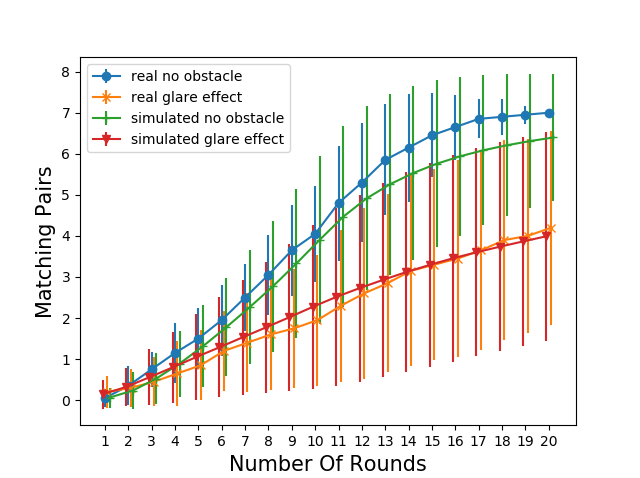
\includegraphics[width=8cm]{images/simulationInitial1.png}
		\caption[Bild kurz]{Add caption}
		\label{fig:simIn1}
	\end{figure}
\end{minipage}
\begin{minipage}{0.5\textwidth}
	\begin{figure}[H]
		\centering
		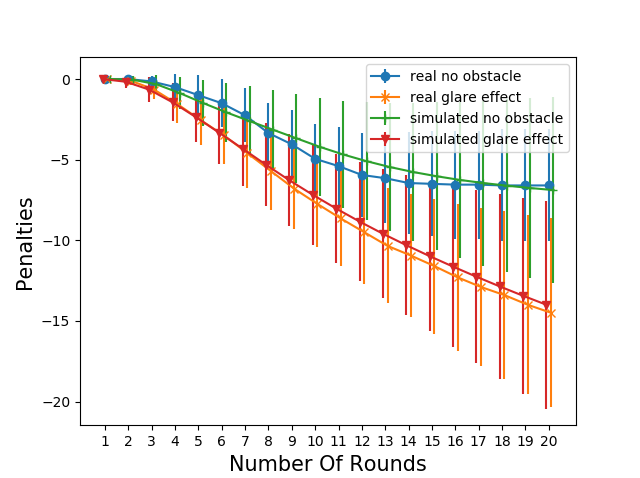
\includegraphics[width=8cm]{images/simulationInitial2.png}
		\caption[Bild kurz]{Add caption}
		\label{fig:simIn2}
	\end{figure}
\end{minipage}

At first glance it can be seen that the simualtions of glare effect games are very similar to the real games, meaning that the constructed similarity matrix creates good simulation results. As a result there is no need to find a different approach for creating the similarity matrix, and no changes to the simulator regarding the simulations of glare effect games are made. However, the simulation of no obstacle games is not quite as accurate. Especially the number of matching pairs after the tenth round in the simulated games is lower than in the real games. Additionally the standard deviation indicated by the whiskers regarding the no obstacle games is noticeably higher in simulated than in the real games. This is not very string in the first turns but gets worse in later turns. Furthermore, however less noticeable, is are the penalties in the simulated games between round 8 and 18 lower than in the real games.

The fact that matching pairs per round for the no obstacle simulations are noticeably lower than in the real games inspired two changes to the simulator. The first one was to introduce a new parameter for the optimization algothithm to optimize. It was called randomizing decy and is a value between 0 and 1, and adresses the problem of worser performance in the löast turn compared to real games. The \textsc{boundary limit}, describing \todo{herausfinden was das ist und erklärung hinzufügen und zuende schrieben}, is multiplied with the randomizing decay each round beginning with the 10th round. This reduces the .. and therefore results in better perfomance in the last 10 steps. The second change was to reduce the probability of revealing a random card (instead of puruing a win strategy) by 0.2 (randomrevealprobabilty is a random value betwen 0 and 1). This was done to increase the overall performance in the simulations by reducing the randomness. The results of these changes can be seen in figure \ref{fig:simOp1} and \ref{fig:simOp2}. 

\begin{minipage}{0.5\textwidth}
	\begin{figure}[H]
		\centering
		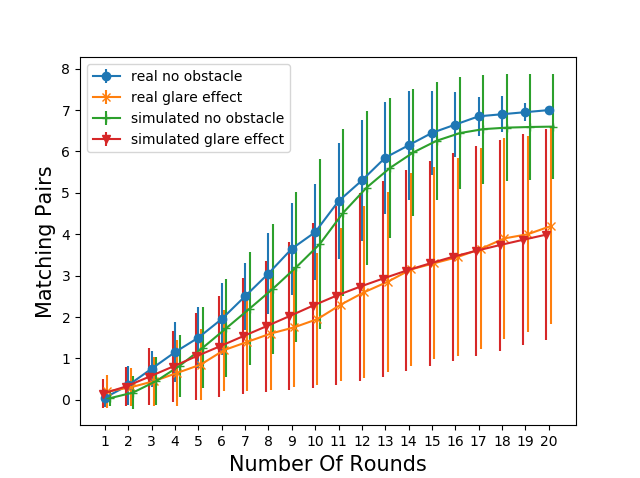
\includegraphics[width=8cm]{images/simulationOptimized1.png}
		\caption[Bild kurz]{Add caption}
		\label{fig:simOp1}
	\end{figure}
\end{minipage}
\begin{minipage}{0.5\textwidth}
	\begin{figure}[H]
		\centering
		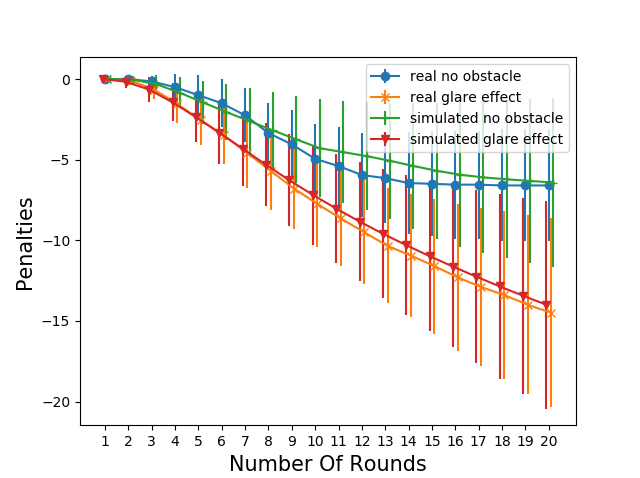
\includegraphics[width=8cm]{images/simulationOptimized2.png}
		\caption[Bild kurz]{Add caption}
		\label{fig:simOp2}
	\end{figure}
\end{minipage} 

As the changes only affected the simulation of no obstacle games, the following statements only refer to those games. It is noticeable that the number of matching pairs per round in the simulated games is closer to the real games. Additionally the standard deviation of the simulated games regarding the matching pairs per round gets noticeably smaller after the 10th round and by that is closer to that in the real games. However, the reduction of randomness also resulted in slightly less penalties after round 10 and by that the differnece in penalties between the simulations and the real games becomes bigger. On the contracry, the standard deviation of the penalties in the last 6 rounds of the simulated no obstacle games got slightliy closer to that in the real games. It seems that the improvements regarding the matching pairs overweight the deteriorations of the penalties, but if these changes actually improve the overall quality of the simulations can not be said without further analysis. 
%will be seen when comparing the classification results before and after the changes. This is done in chapter \todo{ref}. \todo{eigentlich ist das nicht wirklich indiz, vielelict besser: wir untersuchen vorher und nacher mit statistischen test und eventuell auch indication wenn sich die test accuracies unterscheiden später}

However, another interesting observation can be made. The standard deviations of the two perfromance measurements in the last rounds of the simulated no obstacle games is notably higher than in the real games. This might be caused by the fact that there are in generel less or even no cards on the field if all pairs were discovered. This theory also fits to the fact that this is not an issue in the glare effect games, as there are more cards on the field in later turns. This concludes, that there is a possibility that the simulator struggles to accurately simulate rounds once there only a few or no cards remain on the field. 

Although major tendencies of similarities and differences are visually noticable in figure \todo{ref} and figure \todo{ref}, a more accurate analysis is needed to to make reliable statements. Therefore multiple paired samples t-test are performed, comparing real no obstacle, simulated no obstacel, real glare effect and simualted glare effect games with each other. For each combination two tests are performed. One comparing the mean penalties per round and the other one comparing the mean numbers of matching pairs per round. The resulting p values can bee seen in table \todo{ref} and table \todo{ref}. These values express whether the compared lists of mean values are significantly different or not. Values higher than 0.05 indicate no significant difference, while values below 0.05 indicate a significant difference. It would be optimal if all comparissons between different game mode show significant difference, while comparissons between real and simulted games of the same type show no significant difference. All paired sample t-tests were performed before and after the changes to the simulator. This was done to see whether the changes to the simulator improved or deteriorated the results of the test or if they had any impact on them at all. First the results of the paired sample t-tests, when including all 20 rounds and all simulated games, are analysed. Tables \todo{ref} and \todo{ref} show the resuts before changing the simulator, while table \todo{ref} and \todo{ref} show the results afterwards.
%\todo{fertig schreiebn}\\
%It is visble that a improvement to the simulator was made regarding the perfomrance measurements. (ich glaube lkeine statistischen tests fdafür nur wenn ich nopch zeit habe..). Although the graphs show that the simuletad data is very close to the original one, statistcal test will give futher knowledge and certainty. \\
%- t-stochastic test kram (siehe mazens nachricht) -> paired t test: gucken ob no obstacle und glare effet signifikant unterscheidlich sind -> ja sind sie \\
%- vielleicth auch gucken ob verbesserung das signifikant besser gemacht hat, aber kann eventuell auch vernachlässigt werden weil man es visuell sieht und der unterscheid nicht starks sein wird. Dennoch könnte es gut sein dass zu machen. \\
%- auch schriewben was paired ttest überhapt ist und wozu es gut ist.


\begin{table}[H]
	\centering
	\caption{Before change to simulator. p and t values in paired t-test for different comparissons of matching pairs per round. All 1000 simulated games per real game were used. The following abreviatrions are used: real glare effect - r\_g, real no obstacle - r\_n, simulated glare effect - s\_g, simulated no obstacle - s\_n}
	\resizebox{\columnwidth}{!}{%
		\begin{tabular}{|c||ccccc|ccccc|ccccc|}
			
			\hline
			&&& s\_n &&&&& s\_g &&&&& r\_n  && \\
			\hline
			&& p && t &&& p && t &&& p && t & \\
			\hline\hline
			r\_g &&  $1.7e-06$  && $ -6.8179$ &&&  \textcolor{mygreen}{$0.0688$} && $-1.9292$ &&& $9.3e-07$ && $7.1041$ &\\
			r\_n &&   \textcolor{red}{$5.7e-07$}  && $7.3571$ &&& $2.7e-06$ && $6.5765$ &&&     &&     &\\
			s\_g &&  $5.3e-06$  && $6.2480$ &&&  	 &&     &&&     &&     &\\
			\hline
		\end{tabular}
	}
\end{table}




\begin{table}[H]
	\centering
	\caption{Before change to simulator. p ant t values in paired t-test for different comparissons of penalties per round. All 1000 simulated games per real game were used. The following abreviatrions are used: real glare effect - r\_g, real no obstacle - r\_n, simulated glare effect - s\_g, simulated no obstacle - s\_n}
	\resizebox{\columnwidth}{!}{%
		\begin{tabular}{|c||ccccc|ccccc|ccccc|}
			\hline
			&&& s\_n &&&&& s\_g &&&&& r\_n  && \\
			\hline
			&& p && t &&& p && t &&& p && t & \\
			\hline\hline
			r\_g &&  $3.6e-06$  && $-6.4297$ &&&  \textcolor{red}{$1.1e-06$} && $-7.0423$ &&& $3.2e-06$ && $6.4897$ &\\
			r\_n &&   \textcolor{mygreen}{$0.2011$}  && $-1.3242$ &&& $5.6e-06$ && $6.2238$ &&&     &&     &\\
			s\_g &&  $5.4e-06$  && $6.2394$ &&&  	 &&     &&&     &&     &\\
			\hline
		\end{tabular}
	}
\end{table}

\begin{table}[H]
	\centering
	\caption{p and t values in paired t-test for different comparissons of matching pairs per round. All 1000 simulated games per real game were used. The following abreviatrions are used: real glare effect - r\_g, real no obstacle - r\_n, simulated glare effect - s\_g, simulated no obstacle - s\_n}
	\resizebox{\columnwidth}{!}{%
		\begin{tabular}{|c||ccccc|ccccc|ccccc|}
			\hline
			&&& s\_n &&&&& s\_g &&&&& r\_n  && \\
			\hline
			&& p && t &&& p && t &&& p && t & \\
			\hline\hline
			r\_g &&  $5.7e-06$  && $-6.2181$ &&& \textcolor{mygreen}{$0.0688$} && $-1.9292$ &&& $9.3e-07$ && $7.1041$ &\\
			r\_n &&  \textcolor{red}{$1.8e-10$}  && $12.2469$ &&& $2.7e-06$ && $6.5765$ &&&     &&     &\\
			s\_g &&  $1.7e-05$  && $5.7107$ &&&  	 &&     &&&     &&     &\\
			\hline
		\end{tabular}
	}
\end{table}




\begin{table}[H]
	\centering
	\caption{p ant t values in paired t-test for different comparissons of penalties per round. All 1000 simulated games per real game were used. The following abreviatrions are used: real glare effect - r\_g, real no obstacle - r\_n, simulated glare effect - s\_g, simulated no obstacle - s\_n}
	\resizebox{\columnwidth}{!}{%
		\begin{tabular}{|c||ccccc|ccccc|ccccc|}
			\hline
			&&& s\_n &&&&& s\_g &&&&& r\_n  && \\
			\hline
			&& p && t &&& p && t &&& p && t & \\
			\hline\hline
			r\_g &&  $4.8e-06$  && $-6.2967$ &&& \textcolor{red}{$1.1e-06$} && $-7.0423$ &&& $3.2e-06 $ && $6.4897 $ &\\
			r\_n &&  \textcolor{red}{$0.0195$}  && $-2.5519 $ &&& $5.6e-06$ && $6.2238$ &&&     &&     &\\
			s\_g &&  $7.2e-06$  && $6.1045$ &&&  	 &&     &&&     &&     &\\
			\hline
		\end{tabular}
	}
\end{table}


\begin{comment}
\begin{table}[H]
\centering
\caption{p and t values in paired t-test for different comparissons of matching pairs per round. All 1000 simulated games per real game were used. The following abreviatrions are used: real glare effect - r\_g, real no obstacle - r\_n, simulated glare effect - s\_g, simulated no obstacle - s\_n}%\label{tab1}
\begin{tabular}{|c|c|c|c|}
\hline
& s\_n  	&  s\_g  & r\_n 		\\
\hline
r\_g 	&$p=5.7e-06$ &\textcolor{mygreen}{$0.0688$}&$9.3e-07$			\\
r\_n 	&\textcolor{red}{$1.8e-10$}&$2.7e-06$&		  			\\
s\_g 	&$1.7e-05$&			&		  			\\
\hline
\end{tabular}
\end{table}

\begin{table}[H]
\centering
\caption{p values in paired t-test for different comparissons of penalties per round. All 1000 simulated games per real game were used. The following abreviatrions are used: real glare effect - r\_g, real no obstacle - r\_n, simulated glare effect - s\_g, simulated no obstacle - s\_n}%\label{tab1}
\begin{tabular}{|c|c|c|c|}
\hline
& s\_n  	&  s\_g  & r\_n 		\\
\hline
r\_g 	&$4.8e-06$&\textcolor{red}{$1.1e-06$}&$3.2e-06$			\\
r\_n 	&\textcolor{red}{$0.0195$}&$5.6e-06$&		  			\\
s\_g 	&$7.2e-06$&			&		  			\\
\hline
\end{tabular}
\end{table}
\end{comment}

It can be seen that all tests comparing different game mods show significant difference in penalties per round as well as matching pairs per round, which is desired. However significant difference is not dersired in the four test comparing real and simulated games of the same mode, which are highlighted by colours. Before the changes to the simulator, the matching pairs per round in simulated and real no obstacle games show significant differneces. The same goes for the penalties per round in simulated and real glare effect games. As the changes to the simulator only affected the simulation of no obstacle games the significant difference between the matchiung pairs in simulated and real glare effect games prevales. Despite the fact that the matching pairs per round in simulated no obstacle games seem closer to the real games in table figure \todo{ref}, the statistical tests still show a significant differnece between them. Additionally, the small deterioration of the penalties that were caused by the changes to the simulator and can be observed in figure \todo{ref}, led to a significant difference in the penalties per round between simulated and real no obstacle games. Before the changes to the simulator this difference was not significant.  

In total, before the changes to the simulator 2 out of 4 tests comparing games of the same mode, result in undesired significant differences. After the changes to the simulator this increased to 3 out of 4 tests. However, this does not lead to the conclusion that the changes to the simulator decreased the quality of the simulations, as the matching pairs per round in simulated no obstacle game got noticeably more accurate. 

\subsection{Search for a better subset of the data}
In the statictical tests in section \todo{ref}, all all 1000 simulations per participant are used. As some simulations are better than others, using a subset only containing a number of best simulations could lead to further findings. Since the simulated games are sorted by their quality in section \todo{ref}, it is possible to only use a certain number of best simulations for the comparissons, and see whether this improves the undesired properties mentioned above. Furthermore the number of rounds in the comparisson can be changed, so that not all 20 rounds are included. The concideration of including less rounds is of importance, beacuse it can reveal which parts of the game are simulated accurately and which are not. The search for an configuration of those two settings was manually done by varying the number of steps and the ratio between simulated and real data. A configuration of those two settings that produces interesting results consisted of using only the best 10 simulated games per game mode from each participant and only including the first 10 rounds of each game. The results before the changes to the simulator can be seen in table \todo{ref} and \todo{ref}, while the results afterwards are shown in table \todo{ref} and \todo{ref}. The two performance measurements after the changes to the simulator when only using the best 10 simulated games per game mode from each participant are aditionally portrayed in figure \todo{ref} and \todo{ref}.

\begin{table}[H]
	\centering
	\caption{Before change to simulator. p and t values in paired t-test for different comparissons of matching pairs per round. For the simualted data only the best 10 simulated logs from each real log are used. Only the first 10 rounds are used. The following abreviatrions are used: real glare effect - r\_g, real no obstacle - r\_n, simulated glare effect - s\_g, simulated no obstacle - s\_n}
	\resizebox{\columnwidth}{!}{%
		\begin{tabular}{|c||ccccc|ccccc|ccccc|}
			\hline
			&&& s\_n &&&&& s\_g &&&&& r\_n  && \\
			\hline
			&& p && t &&& p && t &&& p && t & \\
			\hline\hline
			r\_g &&  $0.0080$  && $-3.3879$ &&& \textcolor{red}{$6.3e-05$} && $7.0000$ &&&  $0.0058$ && $3.5985$ &\\
			r\_n &&   \textcolor{red}{$0.0047$}  && $3.7292$ &&& $0.0038$ && $3.8679$ &&&     &&     &\\
			s\_g &&  $0.0052$  && $3.6587$ &&&  	 &&     &&&     &&     &\\
			\hline
		\end{tabular}
	}
\end{table}

\begin{table}[H]
	\centering
	\caption{Before change to simulator. p values in paired t-test for different comparissons of penalties per round. For the simualted data only the best 10 simulated logs from each real log are used. Only the first 10 rounds are used. The following abreviatrions are used: real glare effect - r\_g, real no obstacle - r\_n, simulated glare effect - s\_g, simulated no obstacle - s\_n}
	\resizebox{\columnwidth}{!}{%
		\begin{tabular}{|c||ccccc|ccccc|ccccc|}
			\hline
			&&& s\_n &&&&& s\_g &&&&& r\_n  && \\
			\hline
			&& p && t &&& p && t &&& p && t & \\
			\hline\hline
			r\_g &&  $0.0024$  && $-4.1873$ &&& \textcolor{red}{$0.0491$} && $2.2730$ &&&  $0.0014$ && $4.5577$ &\\
			r\_n &&  \textcolor{mygreen}{$0.9426$}  && $0.0740$ &&& $0.0012$ && $4.6629$ &&&     &&     &\\
			s\_g &&  $0.0020$  && $4.2932$ &&&  	 &&     &&&     &&     &\\
			\hline
		\end{tabular}
	}
\end{table}

\begin{table}[H]
	\centering
	\caption{p and t values in paired t-test for different comparissons of matching pairs per round. For the simualted data only the best 10 simulated logs from each real log are used. Only the first 10 rounds are used. The following abreviatrions are used: real glare effect - r\_g, real no obstacle - r\_n, simulated glare effect - s\_g, simulated no obstacle - s\_n}
	\resizebox{\columnwidth}{!}{%
		\begin{tabular}{|c||ccccc|ccccc|ccccc|}
			\hline
			&&& s\_n &&&&& s\_g &&&&& r\_n  && \\
			\hline
			&& p && t &&& p && t &&& p && t & \\
			\hline\hline
			r\_g &&  $0.0064$  && $-3.5291$ &&& \textcolor{red}{$1.5e-05$} && $8.3768$ &&& $ 0.0058$ && $3.5985$ &\\
			r\_n &&  \textcolor{mygreen}{$0.0882$}  && $1.9120$ &&& $0.0039$ && $3.8430$ &&&     &&     &\\
			s\_g &&  $0.0044$  && $3.7734$ &&&  	 &&     &&&     &&     &\\
			\hline
		\end{tabular}
	}
\end{table}

\begin{table}[H]
	\centering
	\caption{p values in paired t-test for different comparissons of penalties per round. For the simualted data only the best 10 simulated logs from each real log are used. Only the first 10 rounds are used. The following abreviatrions are used: real glare effect - r\_g, real no obstacle - r\_n, simulated glare effect - s\_g, simulated no obstacle - s\_n}
	\resizebox{\columnwidth}{!}{%
		\begin{tabular}{|c||ccccc|ccccc|ccccc|}
			\hline
			&&& s\_n &&&&& s\_g &&&&& r\_n  && \\
			\hline
			&& p && t &&& p && t &&& p && t & \\
			\hline\hline
			r\_g &&  $0.0020$  && $-4.3052$ &&& \textcolor{mygreen}{$0.0564$} && $2.1881$ &&& $0.0014$ && $4.5577$ &\\
			r\_n &&  \textcolor{mygreen}{$0.9005$}  && $-0.1286$ &&& $0.0012$ && $4.6771$ &&&     &&     &\\
			s\_g &&  $0.0017$  && $4.4200$ &&&  	 &&     &&&     &&     &\\
			\hline
		\end{tabular}
	}
\end{table}

\begin{comment}
\begin{table}[H]
\centering
\caption{p values in paired t-test for different comparissons of matching pairs per round. For the simualted data only the best 10 simulated logs from each real log are used. Only the first 10 rounds are used. The following abreviatrions are used: real glare effect - r\_g, real no obstacle - r\_n, simulated glare effect - s\_g, simulated no obstacle - s\_n}%\label{tab1}
\begin{tabular}{|c|c|c|c|}
\hline
& s\_n    &  s\_g  & r\_n 		\\
\hline
r\_g 	&$0.0064$&\textcolor{red}{$1.5e-05$}&$0.0058$			\\
r\_n 	&\textcolor{mygreen}{$0.0882$}&$0.0039$&		  			\\
s\_g 	&$0.0044$&		  &		  			\\
\hline
\end{tabular}
\end{table}

\begin{table}[H]
\centering
\caption{p values in paired t-test for different comparissons of penalties per round. For the simualted data only the best 10 simulated logs from each real log are used. Only the first 10 rounds are used. The following abreviatrions are used: real glare effect - r\_g, real no obstacle - r\_n, simulated glare effect - s\_g, simulated no obstacle - s\_n}%\label{tab1}
\begin{tabular}{|c|c|c|c|}
\hline
& s\_n    &  s\_g  & r\_n 		\\
\hline
r\_g 	&$0.0020$&\textcolor{mygreen}{$0.0564$}&$0.0014$			\\
r\_n 	&\textcolor{mygreen}{$0.9005$} &$0.0012$ &		  			\\
s\_g 	&$0.0017$&		   &		  			\\
\hline
\end{tabular}
\end{table}
\end{comment}



\begin{minipage}{0.5\textwidth}
	\begin{figure}[H]
		\centering
		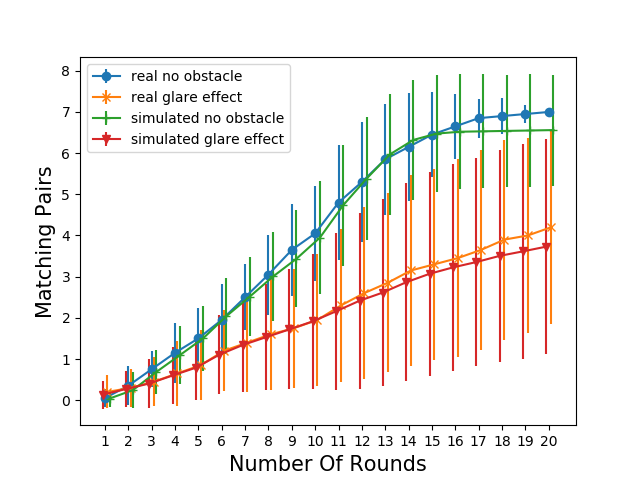
\includegraphics[width=8cm]{images/sd10x/Figure_3.png}
		\caption[Bild kurz]{Add caption}
		\label{fig:simOp101}
	\end{figure}
\end{minipage}
\begin{minipage}{0.5\textwidth}
	\begin{figure}[H]
		\centering
		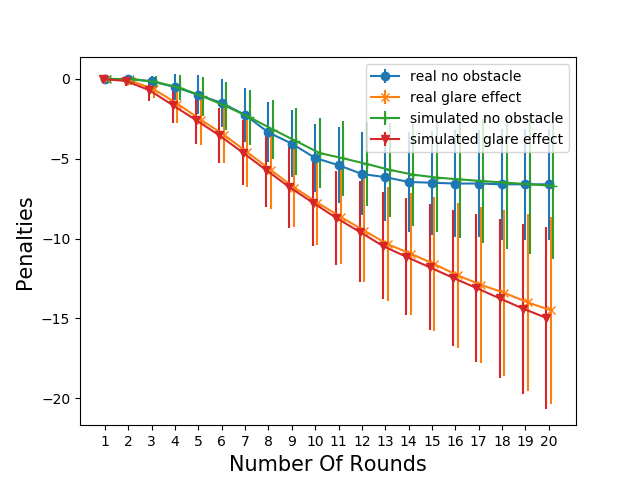
\includegraphics[width=8cm]{images/sd10x/Figure_4.png}
		\caption[Bild kurz]{Add caption}
		\label{fig:simOp102}
	\end{figure}
\end{minipage} 

Interestingly, including all the simulated data in the tests, results in less undesired result before the changes to the simulator compared to afterwards, but using only a small subset of the data results in the opposite. Before the changes to the simulator, when including only the best 10 games and the first 10 rounds in the tests, only one of the 4 tests comparing real and simulated games of the same mode show no significant difference. This is shown in table \todo{ref} and \todo{ref}. Contrary to that, after the changes to the simulator, the test on the chosen subset result in 3 out of those 4 tests show no significant difference. 

As all but one test produce desired results after the changes to the simulator, additional searches for a configuration that only shows desired resultrs were done.
However, such a configuration was not found. If less simulations are used, the three formerly significant differences become insignificant, but the difference in matching pairs bewtween simulated and real glare eeffect games becomes significant. Therefore using the 10 best simulations and the first 10 steps is a good compromise. It should be empghazised that this does not mean that the simulation of the glaree ffect games is bad reagrding the number of matching pairs per round. This only means that the paired sample t-test finds a significant difference in that comparisson. If the two lists of mean values that supposedly are significantly different are manually compared it can be seen that in reality the difference is very small. These values can be seen in table \todo{ref}.

\begin{table}[H]
	\centering
	\caption{mean values of matching pairs for real and simulated games. sd10x. for the first 10 rounds}%\label{tab1}
	\begin{tabular}{|c|c|c|c|c|c|c|c|c|c|c|}
		\hline
		& r1   &  r2  & r3 & r4   &  r5  & r6& r7   &  r8  & r9	&	r10\\
		\hline
		real&0.2 &0.3	&  0.45  &  0.65   &0.85 &  1.2   &    1.4 & 1.6 &  1.75 &1.95	\\
		\hline
		simulated&0.135 &0.27 &	0.405 &0.6  & 0.79 & 1.105& 1.34 & 1.53 & 1.72 & 1.915		\\
		\hline
	\end{tabular}
\end{table}

The highest mean differnece is in round 6 with a differnece of 0.095 matching pairs in that round. This shows that it does not mean that all glare effect simulations used are bad regarding the matching pairs, only because the statistical test finds a significant difference. 
%The fact that the paired sample t-test concludes a significant differnece could be related to the fact that the range of the value sis very small ranging only from .. to .. meaning a samall differnece is much according tpo the ttest..\todo{checken ob das logisch ist, also gucken was der ttest überhaupt macht und das begründen} (auschnitt beschrieben wenn ich weniger nehme.). This would also fit with the fact that using more steps and therefore having a bigger range of values for matching pairs in glare effect games, the difference is not significant (see example where all data is used, ref).

\subsection{Conclusion of the evaluation}
Although no configuration in which all simulations have no significant difference to the according real games regarding the paired sample t-test was found, it can be said that the simulator is capable to simulate the first 10 rounds very accurately, given only the 10 best simulations are used. The statistical tests and the previous consciderations regarding the too large standard deviation in later turns indicate, that the simulator performs less good in later turns. Having said that, these are only indications that would need further tuning and testing of the simulator to be confirmed. Doing so might lead to improving the simulator. 

Regarding the examination whether the changes to the simulator improved the overall quality of the simulations, no clear statement can be made. When all simualted data is used, the paired sample t-tests indicate, that the quality of the simulations may have gotten worse, while when using only the best 10 simulations and only the first 10 rounds, the tests indicate the opposite. 

This analysis also indicates, that it might not ideal to use all simulated data for training as that could results in a significant difference between the simulated and the real games. Using to many simulations compared to real games could decrease the performance of the classifeirs on real data if they adapt too much to simulated games. Furthermore is should be analysed how using differnet amounts of turns in the classification impacts the classification results. In section \todo{ref} different configurations regarding ratios of simulated to real games and the number of rounds includes, are tested. 

Nonetheless it should be emphasized that the aim of no significant difference between real and simuleted games is set very high. Overall the simulations and real games are very similar when comparing them with the two performance measurements. If only the best simulations are used the performance becomes even more similar.  

There are many options in choosing a subset of the data or adjusting the various parameters of the simulator, which could encance the quality of the simulations or reveal further aspects of the simulator that could be improved. In that sense, this analysis does not claim to be complete.

\begin{comment}
	Inhalt...
\end{comment}

\section{Evaluation of simulation}
\label{evaluation_of_simulation}



\subsection{Initial results}
To evaluate whether the performance in the simlated logs is similar to the one in the original logs two perofmance measurements are used: The matching pairs in each round and the penalties in each round. Penalties are given if a card is revealed whose partner has already been seen before but the pair was not picked up. The Initial simulation results can be seen in figure \ref{fig:simIn1} and \ref{fig:simIn2}. The horizontal line extending from the curves, also calles whiskers, describe the standard deviation of the corresponding value. 

\begin{minipage}{0.5\textwidth}
	\begin{figure}[H]
		\centering
		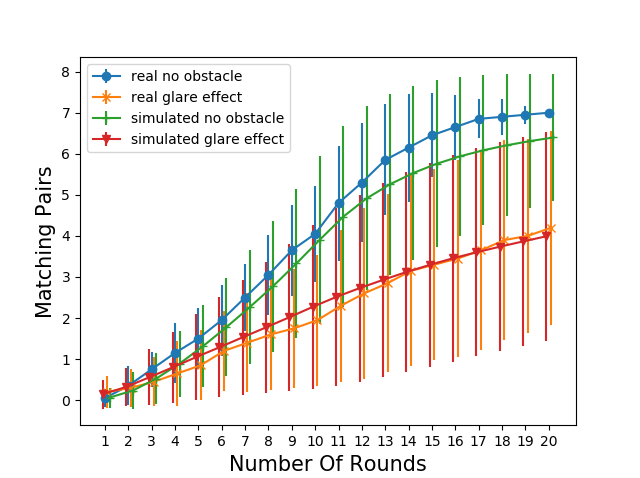
\includegraphics[width=8cm]{images/simulationInitial1.png}
		\caption[Bild kurz]{Add caption}
		\label{fig:simIn1}
	\end{figure}
\end{minipage}
\begin{minipage}{0.5\textwidth}
	\begin{figure}[H]
		\centering
		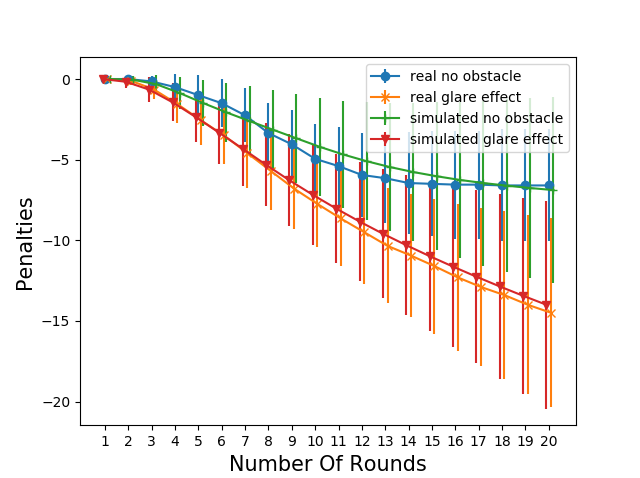
\includegraphics[width=8cm]{images/simulationInitial2.png}
		\caption[Bild kurz]{Add caption}
		\label{fig:simIn2}
	\end{figure}
\end{minipage}

\subsection{Changes to the simulator an the resulting performance of the simulations}
At first glance it can be seen that the simualtions of glare effect games are very similar to the real games, meaning that the constructed similarity matrix creates good simulation results. As a result there is no need to find a different approach for creating the similarity matrix, and no changes to the simulator regarding the simulations of glare effect games are made. However, the simulation of no obstacle games is not quite as accurate. Especially the number of matching pairs after the tenth round in the simulated games is lower than in the real games. Additionally the standard deviation indicated by the whiskers regarding the no obstacle games is noticeably higher in simulated than in the real games. This is not very string in the first turns but gets worse in later turns. Furthermore, however less noticeable, is are the penalties in the simulated games between round 8 and 18 lower than in the real games.

The fact that matching pairs per round for the no obstacle simulations are noticeably lower than in the real games inspired two changes to the simulator. The first one was to introduce a new parameter for the optimization algothithm to optimize. It was called randomizing decy and is a value between 0 and 1, and adresses the problem of worser performance in the löast turn compared to real games. The \textsc{boundary limit}, describing \todo{herausfinden was das ist und erklärung hinzufügen und zuende schrieben}, is multiplied with the randomizing decay each round beginning with the 10th round. This reduces the .. and therefore results in better perfomance in the last 10 steps. The second change was to reduce the probability of revealing a random card (instead of puruing a win strategy) by 0.2 (randomrevealprobabilty is a random value betwen 0 and 1). This was done to increase the overall performance in the simulations by reducing the randomness. The results of these changes can be seen in figure \ref{fig:simOp1} and \ref{fig:simOp2}. 

\begin{minipage}{0.5\textwidth}
	\begin{figure}[H]
		\centering
		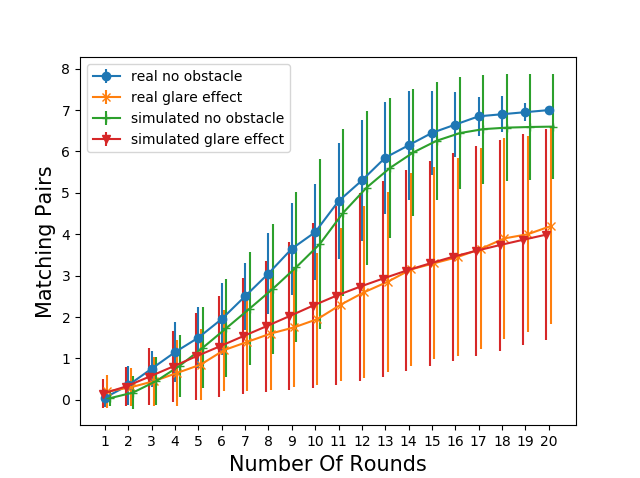
\includegraphics[width=8cm]{images/simulationOptimized1.png}
		\caption[Bild kurz]{Add caption}
		\label{fig:simOp1}
	\end{figure}
\end{minipage}
\begin{minipage}{0.5\textwidth}
	\begin{figure}[H]
		\centering
		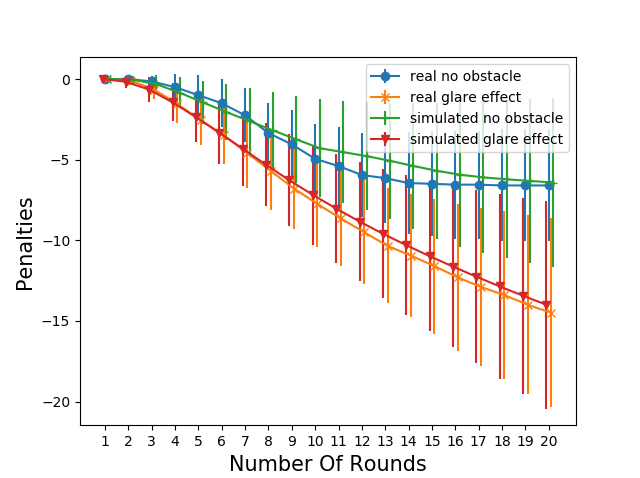
\includegraphics[width=8cm]{images/simulationOptimized2.png}
		\caption[Bild kurz]{Add caption}
		\label{fig:simOp2}
	\end{figure}
\end{minipage} 

As the changes only affected the simulation of no obstacle games, the following statements only refer to those games. It is noticeable that the number of matching pairs per round in the simulated games is closer to the real games. Additionally the standard deviation of the simulated games regarding the matching pairs per round gets noticeably smaller after the 10th round and by that is closer to that in the real games. However, the reduction of randomness also resulted in slightly less penalties after round 10 and by that the differnece in penalties between the simulations and the real games becomes bigger. On the contracry, the standard deviation of the penalties in the last 6 rounds of the simulated no obstacle games got slightliy closer to that in the real games. It seems that the improvements regarding the matching pairs overweight the deteriorations of the penalties, but if these changes actually improve the overall quality of the simulations will be seen when comparing the classification results before and after the changes. This is done in chapter \todo{ref}. \todo{eigentlich ist das nicht wirklich indiz, vielelict besser: wir untersuchen vorher und nacher mit statistischen test und eventuell auch indication wenn sich die test accuracies unterscheiden später}

The higher standard deviations of the two perfromance measurements in the last rounds of the simulated no obstacle games might be caused by the fact that there are in generel less or even no cards on the field if all pairs were discovered. This theory also fits to the fact that this is not an issue in the glare effect games, as there are more cards on the field in later turns. This concludes, that there is a possibility that the simulator struggles to accurately simulate rounds once there only a few or no cards remain on the field. 

\subsection{Statistical Tests}
Although major tendencies of similarities and differences are visually noticable in figure \todo{ref} and figure \todo{ref}, a more accurate analysis is needed to to make reliable statements. Therefore multiple paired samples t-test are performed, comparing real no obstacle, simulated no obstacel, real glare effect and simualted glare effect games with each other. For each combination two tests are performed. One comparing the mean penalties per round and the other one comparing the mean numbers of matching pairs per round. The resulting p values can bee seen in table \todo{ref} and table \todo{ref}. These values express whether the compared lists of mean values are significantly different or not. Values higher than 0.05 indicate no significant difference, while values below 0.05 indicate a significant difference. It would be optimal if all comparissons between different game mode show significant difference, while comparissons between real and simulted games of the same type show no significant difference. All paired sample t-tests were performed before and after the changes to the simulator. This was done to see whether the changes to the simulator improved or deteriorated the results of the test or if they had any impact on them at all. The results ... \todo{beschrieben ob es einen unterschied gibt, und tabellen für vor änderung einbauen}


\todo{das muss ich irgendiwe anders einbauen, besser und verständlicher struktur der subsections}
%\todo{fertig schreiebn}\\
%It is visble that a improvement to the simulator was made regarding the perfomrance measurements. (ich glaube lkeine statistischen tests fdafür nur wenn ich nopch zeit habe..). Although the graphs show that the simuletad data is very close to the original one, statistcal test will give futher knowledge and certainty. \\
%- t-stochastic test kram (siehe mazens nachricht) -> paired t test: gucken ob no obstacle und glare effet signifikant unterscheidlich sind -> ja sind sie \\
%- vielleicth auch gucken ob verbesserung das signifikant besser gemacht hat, aber kann eventuell auch vernachlässigt werden weil man es visuell sieht und der unterscheid nicht starks sein wird. Dennoch könnte es gut sein dass zu machen. \\
%- auch schriewben was paired ttest überhapt ist und wozu es gut ist.


\begin{table}[H]
	\centering
	\caption{p and t values in paired t-test for different comparissons of matching pairs per round. All 1000 simulated games per real game were used. The following abreviatrions are used: real glare effect - r\_g, real no obstacle - r\_n, simulated glare effect - s\_g, simulated no obstacle - s\_n}
	\resizebox{\columnwidth}{!}{%
		\begin{tabular}{|c||ccccc|ccccc|ccccc|}
			\hline
				&&& s\_n &&&&& s\_g &&&&& r\_n  && \\
			\hline
			&& p && t &&& p && t &&& p && t & \\
			\hline\hline
			r\_g &&  $5.7e-06$  && $-6.2181$ &&& \textcolor{mygreen}{$0.0688$} && $-1.9292$ &&& $9.3e-07$ && $7.1041$ &\\
			r\_n &&  \textcolor{red}{$1.8e-10$}  && $12.2469$ &&& $2.7e-06$ && $6.5765$ &&&     &&     &\\
			s\_g &&  $1.7e-05$  && $5.7107$ &&&  	 &&     &&&     &&     &\\
			\hline
		\end{tabular}
	}
\end{table}




\begin{table}[H]
	\centering
	\caption{p ant t values in paired t-test for different comparissons of penalties per round. All 1000 simulated games per real game were used. The following abreviatrions are used: real glare effect - r\_g, real no obstacle - r\_n, simulated glare effect - s\_g, simulated no obstacle - s\_n}
	\resizebox{\columnwidth}{!}{%
		\begin{tabular}{|c||ccccc|ccccc|ccccc|}
			\hline
			&&& s\_n &&&&& s\_g &&&&& r\_n  && \\
			\hline
			&& p && t &&& p && t &&& p && t & \\
			\hline\hline
			r\_g &&  $4.8e-06$  && $-6.2967$ &&& \textcolor{red}{$1.1e-06$} && $-7.0423$ &&& $3.2e-06 $ && $6.4897 $ &\\
			r\_n &&  \textcolor{red}{$0.0195$}  && $-2.5519 $ &&& $5.6e-06$ && $6.2238$ &&&     &&     &\\
			s\_g &&  $7.2e-06$  && $6.1045$ &&&  	 &&     &&&     &&     &\\
			\hline
		\end{tabular}
	}
\end{table}


\begin{comment}
	\begin{table}[H]
	\centering
	\caption{p and t values in paired t-test for different comparissons of matching pairs per round. All 1000 simulated games per real game were used. The following abreviatrions are used: real glare effect - r\_g, real no obstacle - r\_n, simulated glare effect - s\_g, simulated no obstacle - s\_n}%\label{tab1}
	\begin{tabular}{|c|c|c|c|}
	\hline
	& s\_n  	&  s\_g  & r\_n 		\\
	\hline
	r\_g 	&$p=5.7e-06$ &\textcolor{mygreen}{$0.0688$}&$9.3e-07$			\\
	r\_n 	&\textcolor{red}{$1.8e-10$}&$2.7e-06$&		  			\\
	s\_g 	&$1.7e-05$&			&		  			\\
	\hline
	\end{tabular}
	\end{table}
	
	\begin{table}[H]
	\centering
	\caption{p values in paired t-test for different comparissons of penalties per round. All 1000 simulated games per real game were used. The following abreviatrions are used: real glare effect - r\_g, real no obstacle - r\_n, simulated glare effect - s\_g, simulated no obstacle - s\_n}%\label{tab1}
	\begin{tabular}{|c|c|c|c|}
	\hline
	& s\_n  	&  s\_g  & r\_n 		\\
	\hline
	r\_g 	&$4.8e-06$&\textcolor{red}{$1.1e-06$}&$3.2e-06$			\\
	r\_n 	&\textcolor{red}{$0.0195$}&$5.6e-06$&		  			\\
	s\_g 	&$7.2e-06$&			&		  			\\
	\hline
	\end{tabular}
	\end{table}
\end{comment}

It can be seen that all tests comparing different game mods show significant difference in penalties per round as well as matching pairs per round, which is desired. However significant difference is not dersired in the four test comparing real and simulated games of the same mode, which are highlighted by colours. The only test showing no significant difference it the one between matching pairs per round in real and simulated glare effect games, highlighted in green. The other three tests express undesired significant differences between real games and their simulations. As the simulated games are sorted by their quality in section \todo{ref}, it is possible to only use a certain number of best simulations for the comparissons, and see whether this improves the undesired properties mentioned above. Furthermore the number of rounds in the comparisson can be changed, so that not all 20 rounds are included. The concideration of including less rounds is of importance, beacuse it can reveal which parts of the game are simulated accurately and which are not. The search for an better configuration of those two settings was manually done by varying the number of steps and the ratio between simulated and real data. The aim was to inlude as many simulatins and steps as possible while achieving significant differences only in tests where it is desired. A configuration that was better in the sense of achieving this aim consisted of using only the best 10 simulated games per game mode from each participant and only including the first 10 rounds of each game. The results can be seen in table \todo{ref} and \todo{ref}. The two performance measurements whn only using the best 10 simulated games per game mode from each participant are aditionally portrayed in figure \todo{ref} and \todo{ref}.

\begin{table}[H]
	\centering
	\caption{p and t values in paired t-test for different comparissons of matching pairs per round. For the simualted data only the best 10 simulated logs from each real log are used. Only the first 10 rounds are used. The following abreviatrions are used: real glare effect - r\_g, real no obstacle - r\_n, simulated glare effect - s\_g, simulated no obstacle - s\_n}
	\resizebox{\columnwidth}{!}{%
		\begin{tabular}{|c||ccccc|ccccc|ccccc|}
			\hline
			&&& s\_n &&&&& s\_g &&&&& r\_n  && \\
			\hline
			&& p && t &&& p && t &&& p && t & \\
			\hline\hline
			r\_g &&  $0.0064$  && $-3.5291$ &&& \textcolor{red}{$1.5e-05$} && $8.3768$ &&& $ 0.0058$ && $3.5985$ &\\
			r\_n &&  \textcolor{mygreen}{$0.0882$}  && $1.9120$ &&& $0.0039$ && $3.8430$ &&&     &&     &\\
			s\_g &&  $0.0044$  && $3.7734$ &&&  	 &&     &&&     &&     &\\
			\hline
		\end{tabular}
	}
\end{table}

\begin{table}[H]
	\centering
	\caption{p values in paired t-test for different comparissons of penalties per round. For the simualted data only the best 10 simulated logs from each real log are used. Only the first 10 rounds are used. The following abreviatrions are used: real glare effect - r\_g, real no obstacle - r\_n, simulated glare effect - s\_g, simulated no obstacle - s\_n}
	\resizebox{\columnwidth}{!}{%
		\begin{tabular}{|c||ccccc|ccccc|ccccc|}
			\hline
			&&& s\_n &&&&& s\_g &&&&& r\_n  && \\
			\hline
			&& p && t &&& p && t &&& p && t & \\
			\hline\hline
			r\_g &&  $0.0020$  && $-4.3052$ &&& \textcolor{mygreen}{$0.0564$} && $2.1881$ &&& $0.0014$ && $4.5577$ &\\
			r\_n &&  \textcolor{mygreen}{$0.9005$}  && $-0.1286$ &&& $0.0012$ && $4.6771$ &&&     &&     &\\
			s\_g &&  $0.0017$  && $4.4200$ &&&  	 &&     &&&     &&     &\\
			\hline
		\end{tabular}
	}
\end{table}

\begin{comment}
	\begin{table}[H]
	\centering
	\caption{p values in paired t-test for different comparissons of matching pairs per round. For the simualted data only the best 10 simulated logs from each real log are used. Only the first 10 rounds are used. The following abreviatrions are used: real glare effect - r\_g, real no obstacle - r\_n, simulated glare effect - s\_g, simulated no obstacle - s\_n}%\label{tab1}
	\begin{tabular}{|c|c|c|c|}
	\hline
	& s\_n    &  s\_g  & r\_n 		\\
	\hline
	r\_g 	&$0.0064$&\textcolor{red}{$1.5e-05$}&$0.0058$			\\
	r\_n 	&\textcolor{mygreen}{$0.0882$}&$0.0039$&		  			\\
	s\_g 	&$0.0044$&		  &		  			\\
	\hline
	\end{tabular}
	\end{table}
	
	\begin{table}[H]
	\centering
	\caption{p values in paired t-test for different comparissons of penalties per round. For the simualted data only the best 10 simulated logs from each real log are used. Only the first 10 rounds are used. The following abreviatrions are used: real glare effect - r\_g, real no obstacle - r\_n, simulated glare effect - s\_g, simulated no obstacle - s\_n}%\label{tab1}
	\begin{tabular}{|c|c|c|c|}
	\hline
	& s\_n    &  s\_g  & r\_n 		\\
	\hline
	r\_g 	&$0.0020$&\textcolor{mygreen}{$0.0564$}&$0.0014$			\\
	r\_n 	&\textcolor{mygreen}{$0.9005$} &$0.0012$ &		  			\\
	s\_g 	&$0.0017$&		   &		  			\\
	\hline
	\end{tabular}
	\end{table}
\end{comment}



\begin{minipage}{0.5\textwidth}
	\begin{figure}[H]
		\centering
		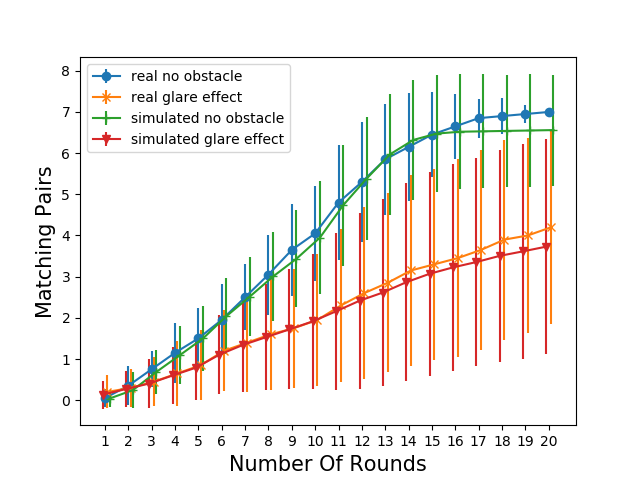
\includegraphics[width=8cm]{images/sd10x/Figure_3.png}
		\caption[Bild kurz]{Add caption}
		\label{fig:simOp101}
	\end{figure}
\end{minipage}
\begin{minipage}{0.5\textwidth}
	\begin{figure}[H]
		\centering
		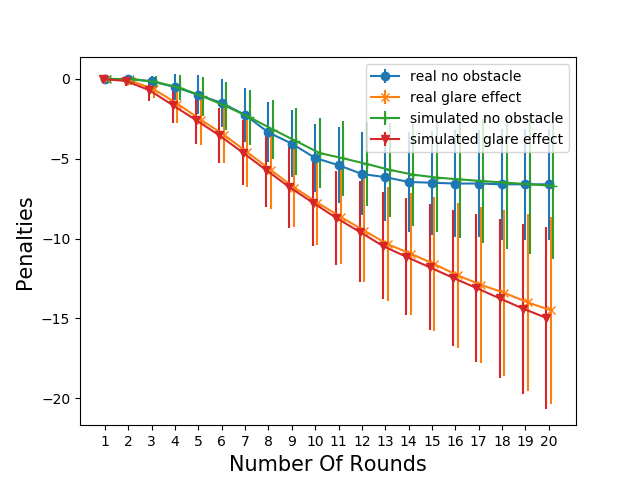
\includegraphics[width=8cm]{images/sd10x/Figure_4.png}
		\caption[Bild kurz]{Add caption}
		\label{fig:simOp102}
	\end{figure}
\end{minipage} 

A configuration that only results in desired outcomes of statistical tests was not found. If less simulations are used, the three formerly significant differences become insignificant, but the difference in matching pairs bewtween simulated and real glare eeffect games becomes significant. Therefore using the 10 best simulations and the first 10 steps is a good compromise. It should be empghazised that this does not mean that the simulation of the glaree ffect games is bad reagrding the number of matching pairs per round. This only means that the paired sample t-test finds a significant difference in that comparisson. If the two lists of mean values that supposedly are significantly different are manually compared it can be seen that in reality the difference is very small. These values can be seen in table \todo{ref}.

\begin{table}[H]
	\centering
	\caption{mean values of matching pairs for real and simulated games. sd10x. for the first 10 rounds}%\label{tab1}
	\begin{tabular}{|c|c|c|c|c|c|c|c|c|c|c|}
		\hline
		& r1   &  r2  & r3 & r4   &  r5  & r6& r7   &  r8  & r9	&	r10\\
		\hline
	 	real&0.2 &0.3	&  0.45  &  0.65   &0.85 &  1.2   &    1.4 & 1.6 &  1.75 &1.95	\\
	 	\hline
	 	simulated&0.135 &0.27 &	0.405 &0.6  & 0.79 & 1.105& 1.34 & 1.53 & 1.72 & 1.915		\\
		\hline
	\end{tabular}
\end{table}

The highest mean differnece is in round 6 with a differnece of 0.095 matching pairs in that round. This shows that it does not mean that all glare effect simulations used are bad regarding the matching pairs, only because the statistical test finds a significant difference. 
%The fact that the paired sample t-test concludes a significant differnece could be related to the fact that the range of the value sis very small ranging only from .. to .. meaning a samall differnece is much according tpo the ttest..\todo{checken ob das logisch ist, also gucken was der ttest überhaupt macht und das begründen} (auschnitt beschrieben wenn ich weniger nehme.). This would also fit with the fact that using more steps and therefore having a bigger range of values for matching pairs in glare effect games, the difference is not significant (see example where all data is used, ref).

Although no clear boundary was found in which all simulations have no significant difference to the according real games regarding the paired sample t-test was found, it can be said that the simulator is capable to simulate the first 10 rounds realistic enough to not be significantly different, given only the 10 best simulations are used.  The statistical tests and the previous consciderations regarding the too large standard deviation in later turns indicate, that the simulator performs less good in later turns. Having said that, these are only indications that would need further tuning and testing of the simulator to be confirmed. Doing so might lead to improving the simulator. 

This analysis also indicates, that it might not ideal to use all simulated data for training as that could results in a significant difference between the simulated and the real games. Using to many simulations compared to real games could decrease the performance of the classifeirs on real data if they adapt too much to simulated games. Furthermore is should be analysed how using differnet amounts of turns in the classification impacts the classification results. In section \todo{ref} different configurations regarding ratios of simulated to real games and the number of rounds includes, are tested. 

Nonetheless it should be emphasized that the aim of no significant difference between real and simuleted games is set very high. Overall the simulations and real games are very similar when comparing them with the two performance measurements. If only the best simulations are used the performance becomes even more similar.   

\newpage

\begin{table}[H]
	\centering
	\caption{Before change to simulator. p and t values in paired t-test for different comparissons of matching pairs per round. All 1000 simulated games per real game were used. The following abreviatrions are used: real glare effect - r\_g, real no obstacle - r\_n, simulated glare effect - s\_g, simulated no obstacle - s\_n}
	\resizebox{\columnwidth}{!}{%
		\begin{tabular}{|c||ccccc|ccccc|ccccc|}
			\hline
			&&& s\_n &&&&& s\_g &&&&& r\_n  && \\
			\hline
			&& p && t &&& p && t &&& p && t & \\
			\hline\hline
			r\_g &&  $1.7e-06$  && $ -6.8179$ &&&  \textcolor{mygreen}{$0.0688$} && $-1.9292$ &&& $9.3e-07$ && $7.1041$ &\\
			r\_n &&   \textcolor{red}{$5.7e-07$}  && $7.3571$ &&& $2.7e-06$ && $6.5765$ &&&     &&     &\\
			s\_g &&  $5.3e-06$  && $6.2480$ &&&  	 &&     &&&     &&     &\\
			\hline
		\end{tabular}
	}
\end{table}




\begin{table}[H]
	\centering
	\caption{Before change to simulator. p ant t values in paired t-test for different comparissons of penalties per round. All 1000 simulated games per real game were used. The following abreviatrions are used: real glare effect - r\_g, real no obstacle - r\_n, simulated glare effect - s\_g, simulated no obstacle - s\_n}
	\resizebox{\columnwidth}{!}{%
		\begin{tabular}{|c||ccccc|ccccc|ccccc|}
			\hline
			&&& s\_n &&&&& s\_g &&&&& r\_n  && \\
			\hline
			&& p && t &&& p && t &&& p && t & \\
			\hline\hline
			r\_g &&  $3.6e-06$  && $-6.4297$ &&&  \textcolor{red}{$1.1e-06$} && $-7.0423$ &&& $3.2e-06$ && $6.4897$ &\\
			r\_n &&   \textcolor{mygreen}{$0.2011$}  && $-1.3242$ &&& $5.6e-06$ && $6.2238$ &&&     &&     &\\
			s\_g &&  $5.4e-06$  && $6.2394$ &&&  	 &&     &&&     &&     &\\
			\hline
		\end{tabular}
	}
\end{table}


\begin{table}[H]
	\centering
	\caption{Before change to simulator. p and t values in paired t-test for different comparissons of matching pairs per round. For the simualted data only the best 10 simulated logs from each real log are used. Only the first 10 rounds are used. The following abreviatrions are used: real glare effect - r\_g, real no obstacle - r\_n, simulated glare effect - s\_g, simulated no obstacle - s\_n}
	\resizebox{\columnwidth}{!}{%
		\begin{tabular}{|c||ccccc|ccccc|ccccc|}
			\hline
			&&& s\_n &&&&& s\_g &&&&& r\_n  && \\
			\hline
			&& p && t &&& p && t &&& p && t & \\
			\hline\hline
			r\_g &&  $0.0080$  && $-3.3879$ &&& \textcolor{red}{$6.3e-05$} && $7.0000$ &&&  $0.0058$ && $3.5985$ &\\
			r\_n &&   \textcolor{red}{$0.0047$}  && $3.7292$ &&& $0.0038$ && $3.8679$ &&&     &&     &\\
			s\_g &&  $0.0052$  && $3.6587$ &&&  	 &&     &&&     &&     &\\
			\hline
		\end{tabular}
	}
\end{table}

\begin{table}[H]
	\centering
	\caption{Before change to simulator. p values in paired t-test for different comparissons of penalties per round. For the simualted data only the best 10 simulated logs from each real log are used. Only the first 10 rounds are used. The following abreviatrions are used: real glare effect - r\_g, real no obstacle - r\_n, simulated glare effect - s\_g, simulated no obstacle - s\_n}
	\resizebox{\columnwidth}{!}{%
		\begin{tabular}{|c||ccccc|ccccc|ccccc|}
			\hline
			&&& s\_n &&&&& s\_g &&&&& r\_n  && \\
			\hline
			&& p && t &&& p && t &&& p && t & \\
			\hline\hline
			r\_g &&  $0.0024$  && $-4.1873$ &&& \textcolor{red}{$0.0491$} && $2.2730$ &&&  $0.0014$ && $4.5577$ &\\
			r\_n &&  \textcolor{mygreen}{$0.9426$}  && $0.0740$ &&& $0.0012$ && $4.6629$ &&&     &&     &\\
			s\_g &&  $0.0020$  && $4.2932$ &&&  	 &&     &&&     &&     &\\
			\hline
		\end{tabular}
	}
\end{table}

\newpage

\section{Feature generation}
\label{feature_generation}

\subsection{1D CNN features}
\label{1d_cnn_features}
For the 1D CNN five statistcal features for each step are used: The card codes, the number of cards left, the number of never revealed cards,  the highest number of times the same card was revealed and the number of steps  since all pairs were found. They are calculated using the game logs from \todo{ref}. These features can be direclty fed into the 1d CNN explained in chapter \todo{ref}. 

The code for calculating the statistal features out of game logs was already given. A script was written that incorparates this funtionality in order to calculate the features for all logs. Additionally, after creating the neccessary directory structure the script saves the files for the splits of the raw data and the features. The reason for saving the features is that they do not have to calculated before evrey training and instead can be loaded from files. The reason for also saving the raw data even though this work does not need them anymore is, that the working group that was collaborated with also trained other models and does not directly load the features but instead caalculates them before each training.

\subsection{2D CNN features}
\label{2d_cnn_features}

For the second approach of using a 2D CNN further steps are taken. Therefore synthetic images in gray scale colours are created using the features mentioned above. As the images are in gray scale colours, only one color channel is needed. One can visually think of this approach as creating graphs for each feature that display their values in each timestep, taking a photograph of each graph and stacking them on top of eachother. This can be clarified by looking at the code that produces the synthetic images.  

\begin{lstlisting}[language=python, caption=Add caption, xleftmargin=5.0ex]
def create_image(game, components=[True, True, True, True, True]):
	'''
	Creates synthetic images out of the five staticial features.
	:param game: The statical features in each step. 
	:param components: Five values describing which of the features 
	should be used to create the image. 
	:return: The synthetic image.
	'''
	card_codes = np.zeros((7, steps))
	cards_left = np.zeros((8, steps))
	never_revealed_cards = np.zeros((14, steps))
	max_same_card_reveals = np.zeros((20, steps))
	rounds_since_done = np.zeros((27, steps))
	
	x_position = 0
	for step in game:
		card_code = math.floor(step[0])
		first_or_second = int(round((step[0] % 1) * 10))
		if card_code != 0:
			card_codes[card_code - 1][x_position] = first_or_second 
		pairs_left[int(step[1] / 2)][x_position] = 1
		never_revealed_cards[int(step[2])][x_position] = 1
		max_same_card_reveals[int(step[3])][x_position] = 1
		rounds_since_done[int(step[4])][x_position] = 1
		x_position += 1
	
	image = np.zeros((0, steps))
	if components[0]:   
		image = np.vstack((image, card_codes))
	if components[1]:
		image = np.vstack((image, max_same_card_reveals))
	if components[2]:  
		image = np.vstack((image, rounds_since_done))
	if components[3]:
		image = np.vstack((image, cards_left))
	if components[4]:   
		image = np.vstack((image, never_revealed_cards))
	
	return image
\end{lstlisting}

By using pseudo colors, the images can be displayed with colours, like in figure \ref{fig:synImOr}. These 76 $\cdot$ 40 $\cdot$ 1 (height $\cdot$ width $\cdot$ colour channels) images are direclty fed to the 2D CNN explained in chapter .. \todo{rerf}. By setting the origin of the image to the lower instead of the upper left corner a more naural looking image is created and can be seen in figure \ref{fig:synIm}. 

\begin{minipage}{0.5\textwidth}
	\begin{figure}[H]
	\centering
	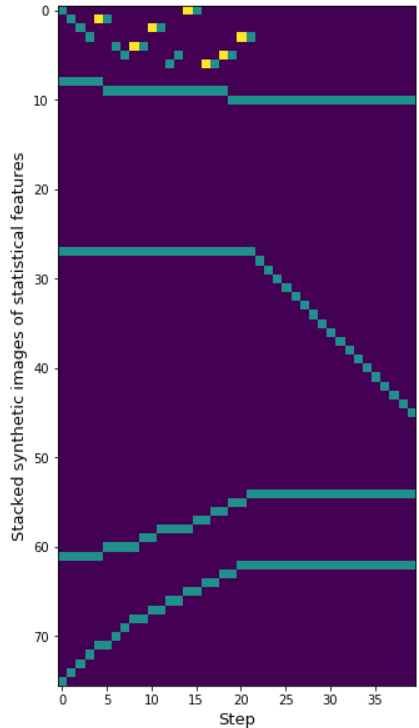
\includegraphics[width=7cm]{images/synImageOriginal.png}
	\caption[Bild kurz]{Add caption}
	\label{fig:synImOr}
\end{figure}
\end{minipage}
\begin{minipage}{0.5\textwidth}
	\begin{figure}[H]
		\centering
		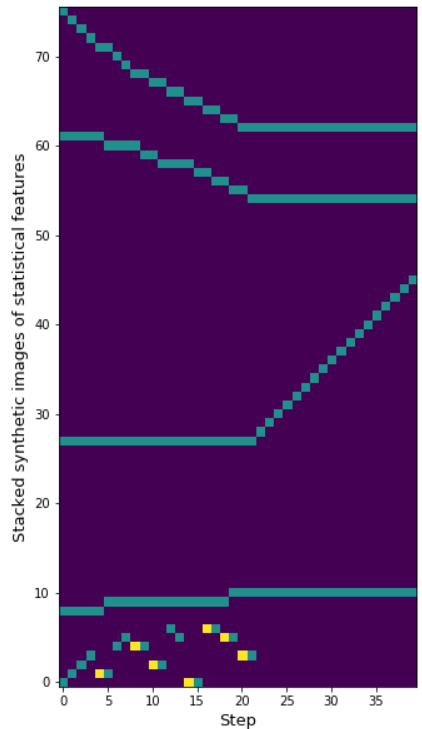
\includegraphics[width=7cm]{images/synImage.png}
		\caption[Bild kurz]{Add caption}
		\label{fig:synIm}
	\end{figure}
\end{minipage}

The width of the image is 40 because that the number of steps recorded. Table \todo{ref} shows which of the areas in the image describe which statical feature. The different vertical spaces given to statistical features were purposefully chosen. The aim was to use as much space as neccessary but as little as possible. As each round consists of two cards being turned face up and the impossibility to chose the same card twice in one turn, a card can be at maximum revealed 20 times during 20 rounds. Considering that this value is at minimum 1 because it is not possible to flip no cards, the range of 20 values is sufficient for this value. Furthermore 14 steps are at minimum needed to complete the game, since there are 14 cards. As a result this value can range from 0 to 26, meaning a vertical space of 27 is needed. In order to save space, the statistcal feature of the number of cards left was converted to the number of pairs left. By dividing by 2 the vertical space neccessary to visualize this feature is halved, without information being lost. Instead of representing the numbers left on the field, the value now represents the number of pairs left. Furthermore the number of never revealed cards can range from 0 to 13. The value 14 is not possible because two cards have to be chosen each turn, meaning that it is impossible to not reveal any card. The stacking order was chosen so that the coloured pixels of different statistical features rarely touch each other. 
\begin{table}[H]
	\centering
	\caption{add caption. Upper and lower boundaries are inclusive.}%\label{tab1}
	\begin{tabular}{|l|l|l|}
		\hline
		Statistical feature & Range & Vertical space in the image \\
		\hline
		Card codes & 1-7 & 0-6 \\
		Maximum of same card reveals & 1-20 & 7-26 \\
		Steps since game ended & 0-26 & 27-53 \\
		Pairs left & 0-7 & 54-61\\
		Never revealed cards & 0-13 & 62-75 \\
		\hline
	\end{tabular}
\end{table}

Regarding the visual representatoin of he card codes two two decisions were made: Using different colours for the first and the second card of a colour and combining the information about the 14 cards in an vertical area of size 7. For each card code the vertical position of the representing pixel is decided by the first number and the colour is chosen according to the second number. As a result each row contains the information about cards of a specific colour. This representation of the card codes is not chosen arbirtrarily. On the contrary, it was inspired by reasons that need explanation.

Insrtead of combining the information about the 14 cards in an vertical area of size 7, it would have been also possible to use double the vertical space so that the first and the second card of a colour each have separate areas. The first cards and the second cards of a colour would each have individual vertical spaces with sizes of 7. However, it was decided against it. This decision was based on a conscideration regarding the way convolutional neural networks function and how they are used in this work. How cnns function is discussed in detail in chapter \todo{ref} and therefore the following explanation is kept short. During a convolution, each filter has a fixed size and step by step walks over the image, extracting features from areas to create a feature map. This means that a neuron in this layer only reacts to stimuli in a local area of the previous layer. \todo{satz selsbt verstehen und gucken ob ich es umschreieb dass es verständlicher ist. auf jeden fall auch in cnn chapter aufgreifen} This behaviour follows the biological model of the receptive field. As cnns consist of multiple layers, the receptive field, and therefore the distance in which dependencies between the pixels in the original input image can be learned, grows with each layer. This also means that if the structure of the cnn is chosen small, its receptive field might not grow enough for the model to learn dependencies between far distant pixels of the original input image. In this work, the 2d cnn used is intentionally constructed with a small number of layers for reasons explained in chapter \todo{ref}. Therefore it is desireable that pixels in between an important dependency can be assumed are close to each other so that the small cnn is able to learn that dependency. %Firstly, more complex structures were tested on the synthetic images and did not show better results, meaning that small networks are sufficient for the task at hand and secondly, less complex models result in shorter training time and by that allow the training of more models. 
Unlike in classical image classification the images used are created synthetically, and in that sense their structure can be chosen freely in the favour of the task at hand. The chosen representation of the card codes exploits exactly this freedom. As the dependencies between cards of the same colours can be estimated to be very important for the classification, the representation is chosen so that if cards of the same colour are flipped in quick succession the pixels describing them are also locally close to each other in the synthetic image. The dependency between such close pixels does not require a large receptive field in order to be learned by the network. Therefore this representation is better suited for the small structure of the cnn that is being utilized. 




%a representation is chosen in which pixels describing cards of the same colour are in the same row and have different colours depending on if it is the first or second card of that colour. As a result, . Additionally these visual  properties are less complex than they would have been in the other approach and are therefore more 

%when conscidering how convoluntions in 2d cnns are performed, this approach seems less promissing. During the convolutions, each filter has a fixed size and step by step walks over the image, extracting features from areas to create a feature map \todo{ref to cnn chapter}. This means that the extracted features during a convolution and therefore the gained knowledge of the model depends on the information found in areas with the size of the filter. Regarding the topic at hand, chossing individual areas for the card codes would create a significant distance between the pixels describing the first and second card of a colour. In order to extract features during the convolution that capture the connection between those distaned pixels, the filter size would need to be at least as big as the distance. This results in large areas that include many different pixels overshadowing the importance of the two specific pixels  describing the first and the second card of a color and thereby making it harder for the model to learn the connection between them. Hence, the approach of doubling the vertical space results in high unlikelyness of the model learning this characteristic. Contrary to that, using a combined space and different colours results in spatial proximity of the pixels describing the desired characteristic, which can therefore be captured by smaller filter sizes. In conlusion, chossing a representation for the card codes that contains local features and using a small filter size, results in a higher likelyness of capturing the desired characteristics. 

The main reason that motivated the use of different colours derived from the first decision to combine information about 14 cards in a vertical space of 7. If the same colour was used for all card codes, there would be no visual differnece between flipping the same card in consequtive turns and flipping two different cards with the same colour. This of course would also mean that the model could not differentiate bewteen those two cases, although they stem from completely differnet behaviour. Using different colours for the first and the second card of a colour fixes this issue. Furthermore the colours visually emphasize some behavioural characteristics that could be helpful for the eventual classifier. By comparing the the card code sections of two images from which one is created using a glare effect and the other one with a no obstacle game, using different colours results in noticeably different visual representations. 
\begin{figure}[H]
	\centering
	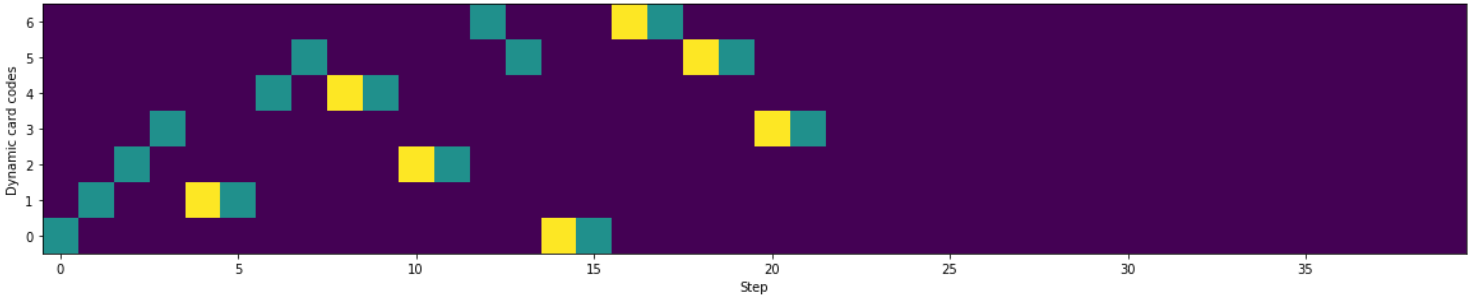
\includegraphics[width=15cm]{images/cardCodesNoObst.png}
	\caption[Bild kurz]{Add caption}
	\label{fig:ccNo}
\end{figure}
\begin{figure}[H]
	\centering
	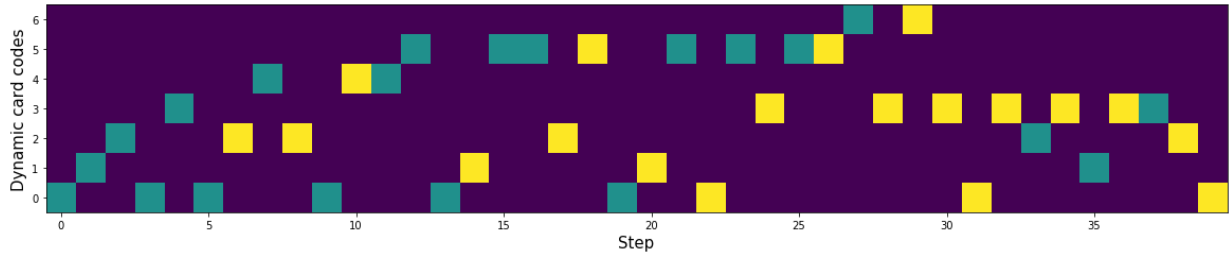
\includegraphics[width=15cm]{images/cardCodesGlare.png}
	\caption[Bild kurz]{Add caption}
	\label{fig:ccGlare}
\end{figure}
In \ref{fig:ccNo}, showing the image for an no obstacle game, there are yellow pixels directly left of green ones, meaning that the probant flipped a card, knew that he had already seen the matching card and direclty flipped it. However, this happens less often in figure \ref{fig:ccGlare} which shows the image for an glare effect game. This is not the case in every game, but the theory is that separations of different coloured cells in the image are more likely in glare effect games than in no obstacel games. Therefore it could be beneficial for the model to learn these characteristics. It should be noted that what the cnn exactly learns or what exact influence the chosen representation has can only be speculated. 

%It could be argued that simply using a vertical space of 14 and changing the order of the rows so that rows describing cards of the same colours are next to each other would have been an easier solution. However, this would firstly be contradicting to the aim using as little space as neccessary and secondly would exclude the possibility of emphasized behavioural characteristics that 

Especially the uncertainty in the influence of the different colours shows, that the approach of creating synthetic images is very experimental. There is no such thing as a standard approach in creating synthetic images for cnns. At least there is none, yet. Although the way cnns function can be conscidered when deciding how to create the synthetic image, this does not guarantee good classification results.


\begin{comment}
	The idea behind using different colours for the first and the second card of a colour is that this vizualizes important behavioural characteristics that help deciding whether the visual obstacle being the sunlight is involved or not. By comparing the the card code sections of two images from which one is created using a glare effect and the other one with a no obstacle game, the different colours result in a noticeably . 
	\begin{figure}[H]
	\centering
	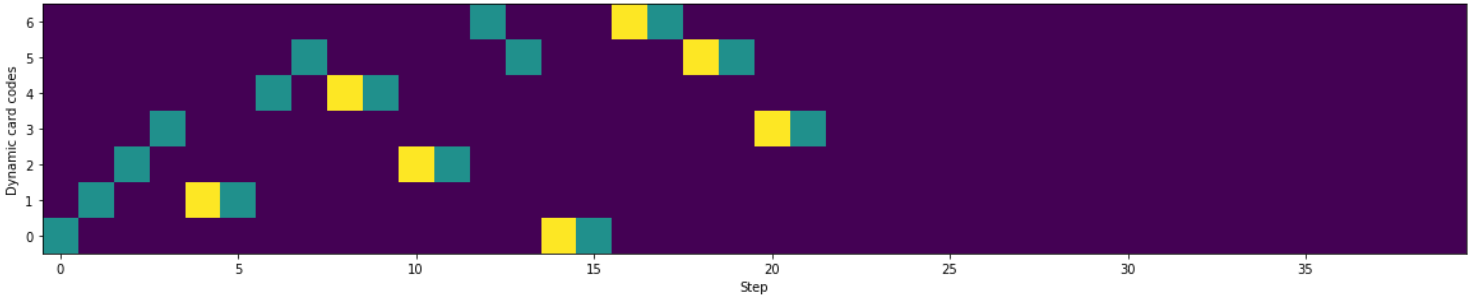
\includegraphics[width=15cm]{images/cardCodesNoObst.png}
	\caption[Bild kurz]{Add caption}
	\label{fig:ccNo}
	\end{figure}
	\begin{figure}[H]
	\centering
	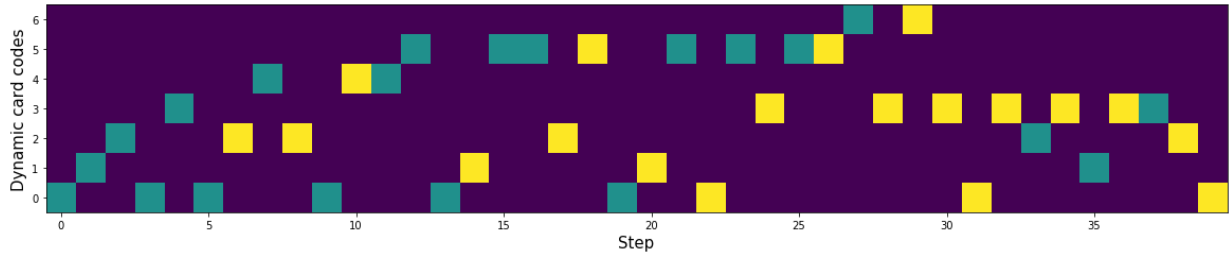
\includegraphics[width=15cm]{images/cardCodesGlare.png}
	\caption[Bild kurz]{Add caption}
	\label{fig:ccGlare}
	\end{figure}
	
	In \ref{fig:ccNo}, showing the image for an no obstacle game, there are yellow pixels directly left of green ones, meaning that the probant flipped a card, knew that he had already seen the matching card and direclty flipped it. However, this happens less often in figure \ref{fig:ccGlare} which shows the image for an glare effect game. This is not the case in every game, but the theory is that separations of different coloured cells in the image are more likely in glare effect games than in no obstacel games. Therefore it could be beneficial for the model to also learn these characteristics. If the same colour was used for all card codes, there would be no visual differnece between flipping the same card in consequtive turns and flipping two different cards with the same colour. This of course would also mean that the model could not differentiate bewteen those two cases.
	
	It 
\end{comment}

umschrieben: grund ist, dass es zusätzliche characteristekn des spiels visualisiert, die von den convolutional genauer gesgat dem rezepivem feld erfasst werden können. ... zeigen und erklären .. bei 14 reihen und getrennt jeweils für erste ode zweite wären die pixel die gefundene paare beschrieben nicht in der nähe voneonader. Ein kleines rezeptive feld würde könnte den zusammenhanmg nicht erfassen. Und selbst wenn man ein größeres wählt gibt es in dem bereich des feldes dann deutlich mehr pixel mit dem selben farben die den wichtigen zusammenhang zwischen 2 spezifischen pixeln in den schatten stellen könnten. Würde man gleiche farben benutzen gäbe es keinen untershcied zwischen zweimal die selbe karte in nah einanderfolgenden zügen und die zueinandergehörigen beiden karetn. Es heißt jedoch nicht dass das netz nicht in der lage ist featurees (oder so) aus verschiedenen bereichen in verbindung zu setzen. Ganz im gegenteil: die fullyy connected oder auch dense layer tun genau dies. Jedoch suchen sich die fully connected layer quasi die feautures aus dem letzen vorherigen layer aus die wichtig sind. Aber angenommen die beiden angesprochen pixel sind sich nicht nah genug um vom rezeptiven field erfasst zu werden und zwischen den beiden pixeln bzw. generell in dem bereich der card codes sind noch viele weitere solcher pixel, dann gibt es keine features die den zusammenhang enthalten und die aufgabe diesem ztusammenhang zu finden liegt dann an den dense layern. Das die dense layer einen zusammenhang zwischen genau den beiden pixln finden und das für gänzlich unterschiedliche card code bereiche je spiel ist äußerst undwahrscheinlciu. \todo{das muss biscchen genauer und verständlicher alles.}

\todo{text}

\todo{vielleicht mit mazen drüber reden ob das sinn ergibt. Ich glaube das ergibt sinn, aber ich müsste nochmal mehr das quellen suchen. Auch mir receptive field und so}

\chapter{Convolutional neural networks}
As convolutional layers are complex and have many variations for differnet use cases, only concepts and functionaslities that are relevant for this work will be covered. This also menas that 3 dimensional cnns will not be explained, but in generel cnns function the same way whether they have 1, 2 or 3 dimensions. The main differnce lies in how the filter, also known as kernel or festure detector, moves acrross the data. This is later explained in more detail. (\todo{ich glaube input data ist keine regel sondern nur meist so..zum beispiel kann man auch 1d convoltion bei 1d, 2d, oder 3d daten machen}). \\
 First of all the core concepts of cnns will be explained and afterwards the models used in this work will be described.\\

On of the core concepts of convoluntional neural networks are the concolutions. \\




Unituitievly, a 2d cnn must not neccerailty have 2 dimensional data as input.

notes bei models:\\
- stride = wie viele schritte auf einmal, default 1 deshalb vermute ich bei mir 1\\
- maxpooling: pool size = 2*2, und bei keras wird stride dann defauklt auch zu 2*2 (=pool size)\\
- input size = 85*40 glaube ich\\
- filter weights are randomly initialized, so that they dont all initially learn the same feauters. To briefly explain the behaviour of filters a seperation bettween two cases can be made: The first case is that not all features of high quality have been learned yet, high quality meaning that learning them would lower the cost function. In that case it is highly unlikely that each filter would begin to resemble other filters, as that would most certainly result in an increase of the cost function and therefore no gradient descent algorithm would head in that direction. The other case is that all features of high quality have already been leanred by a subset of the avaibable filters. In this case the cost function would not be increased if the remaining filters learn similar features than the other filters. \\
- in einem der schritte wird eine zeile usgelassen, aber ich trainiere nicht nochmal alles neu (oder?)\\

- 1d and 2d convolution
- reduction of dimension
- relu 
- number od filter, random initializion, etc
- kernel and kernel size
- loss function and optimizer, stochastic gradeint decent
- Dropout layers
- Pooling, max pooling 
- flatten
- dense relu, softmax
- droput layer, pooling ändert nichts an der anzahl der fetsure maps
- \todo{bessere quelle finden, buch oder so}
- stride (ganz kurz, beschriebt verhalte wenn etwas über bleibt, zero padding oder weglassen)
- back propagation
- wie schaffen die es bspw. 64 feature maps auf 32 zu reduzieren? also wie funktionieren die filter in dem fall? 

  



\chapter{Classification}
\label{classification}

\begin{comment}
	\section{Hardware resources}
	\label{hardwaree recources}
	\todo{vielleicht recources raus lassen}
	
	Multiple servers, provided by the cognitive system lab, were used. One of the provided servers is optimized for storing large amounts of data and was therefore used to store the histories and the results from the models during training while the other servers focus on computing power and were used to execute that training and evaluation. Mainly two servers were used for the training. One has the hardware specification shown in table \todo{ref} and the other one those shown in table \todo{ref}. 
	
	
	\begin{table}[H]
	\centering
	\caption{add caption}
	\label{mll-knecht}
	\resizebox{\columnwidth}{!}{%
	\begin{tabular}{l|ll}
	Component & Model & Additional details                   \\
	\hline
	Processing Unit    & Intel® Xeon® Gold Prozessor 5218      & 64 logical cores, \\
	&									& turbo boosts to 3,90 GHz \\
	System Memory      & -                      	           & 377 GB          \\
	Grafics            & 2 x NVIDIA RTX 2080 ti        		   & 11 GB graphics memory                   
	\end{tabular}
	}
	\end{table}
	
	\begin{table}[H]
	\centering
	\caption{add caption}
	\label{rechenknecht2}
	\resizebox{\columnwidth}{!}{%
	\begin{tabular}{l|ll}
	Component & Model & Additional details                   \\
	\hline
	Processing Unit    & Intel® Xeon® Prozessor E5-2650 v4     & 24 logical cores, \\
	&									& turbo boosts to 2,90 GHz \\
	System Memory      & -                      	           & 252 GB          \\
	Grafics            & NVIDIA GTX 1080 ti        		   & 11 GB graphics memory                   
	\end{tabular}
	}
	\end{table}
	
	\todo{specs nochmal checken sobald ich ins cartesium kann und da nachfragen. vor allem grafikkarte und hesteller des rams}
\end{comment}



\section{Models}
\label{models}
For determining whether subjects played a game without any obstacles or a game effected by the glare effect, one dimensional and two dimensional convolutional neural networks are utilized. As the task at hand is naturally a sequence classification, using 1D convnets is the more conventional approach of the two. 2D convnets on the other hand hand are almost universally used in computer vision applications \cite[Chapter~5]{cnn}. However, a possibility is to create synthetic images from the sequential data and use these images in a 2D convnet \cite{2dcnn}. The synthetic images are created in section \ref{2d_cnn_features} \nameref{2d_cnn_features}. The dimensions of the data and the feature maps in figure \ref{fig:1dCnnStructure} and \ref{fig:2dCnnStructure} are calculated for the case that all 20 rounds are used. If a different number of rounds is used the values differ. 

The models do not necessarily produce the best results possible since best practice 1D convnet \cite{1dcnn} and 2D convnet \cite{2dcnn} topologies are used. As the amount of collected real data with 20 recordings for each label is very limited, it was decided not to split the data into training, test and validation data, and instead only into training and test data using leave-one-out cross validation, where each model is trained with data from n-1 subjects and thus tested on the data from the remaining subject \cite[Chapter~1]{oneOut}. As there is no separate validation set, an optimization would have to be done on the test data. If the parameters are optimized using the test set, the measurement of generalization would be flawed \cite[Chaper~4]{cnn}. Therefore, it was avoided to optimize the hyper parameters individually for each model to ensure generalizing on new testing data. Instead, common best practice hyper parameters were optimized over all the models for better generalizing ability.

%In order to optimize the models a separate validation set would be neccessary. It could be used to tune the hyper parameters of the model and the models would be tested on the test data that was not part of the process of the optimization. 

%The reason why the optimization is done on a separate validation set is, that the models can then be tested on the test data which was not part of the process of selecting the best hyper parameters. If the models were optimized using the test data, the results would not be representitive of the performance of the models on unknown data. 

%The cnn models are intentionally created not very complex for two reasons: Firstly, a lot of training needs to be done with differnet configurations regarding the steps included and the ratios of simulkated to real data. As mentioned in \todo{ref}, 76800 models need to be trained. As the time this work is created in is limited, training that many complex models would take too long. Especially the training of the 2d cnns requires a lot of time. Secondly, to assure that the structures are complex enough, more complex models were exemplary trained and they showed either similar or worse performance. The results of the more complex models can be see in the appendix \todo{ref?}. 

%only difference is input size depending on the number of round included. 

%\todo{statt begründung die quellenangeben. Von wo..}


\begin{comment}
	The visualisations are based (and heavily adjusted) on the latex code provided by the following license:
	
	MIT License
	
	Copyright (c) 2018 HarisIqbal88
	
	Permission is hereby granted, free of charge, to any person obtaining a copy
	of this software and associated documentation files (the "Software"), to deal
	in the Software without restriction, including without limitation the rights
	to use, copy, modify, merge, publish, distribute, sublicense, and/or sell
	copies of the Software, and to permit persons to whom the Software is
	furnished to do so, subject to the following conditions:
	
	The above copyright notice and this permission notice shall be included in all
	copies or substantial portions of the Software.
	
	THE SOFTWARE IS PROVIDED "AS IS", WITHOUT WARRANTY OF ANY KIND, EXPRESS OR
	IMPLIED, INCLUDING BUT NOT LIMITED TO THE WARRANTIES OF MERCHANTABILITY,
	FITNESS FOR A PARTICULAR PURPOSE AND NONINFRINGEMENT. IN NO EVENT SHALL THE
	AUTHORS OR COPYRIGHT HOLDERS BE LIABLE FOR ANY CLAIM, DAMAGES OR OTHER
	LIABILITY, WHETHER IN AN ACTION OF CONTRACT, TORT OR OTHERWISE, ARISING FROM,
	OUT OF OR IN CONNECTION WITH THE SOFTWARE OR THE USE OR OTHER DEALINGS IN THE
	SOFTWARE.
\end{comment}

\newpage

\subsection{1D convnet}
\label{1d_cnn}
The structure of the 1D convnet used is shown in figure \ref{fig:1dCnnStructure}.
\begin{figure}[H]
	\centering
	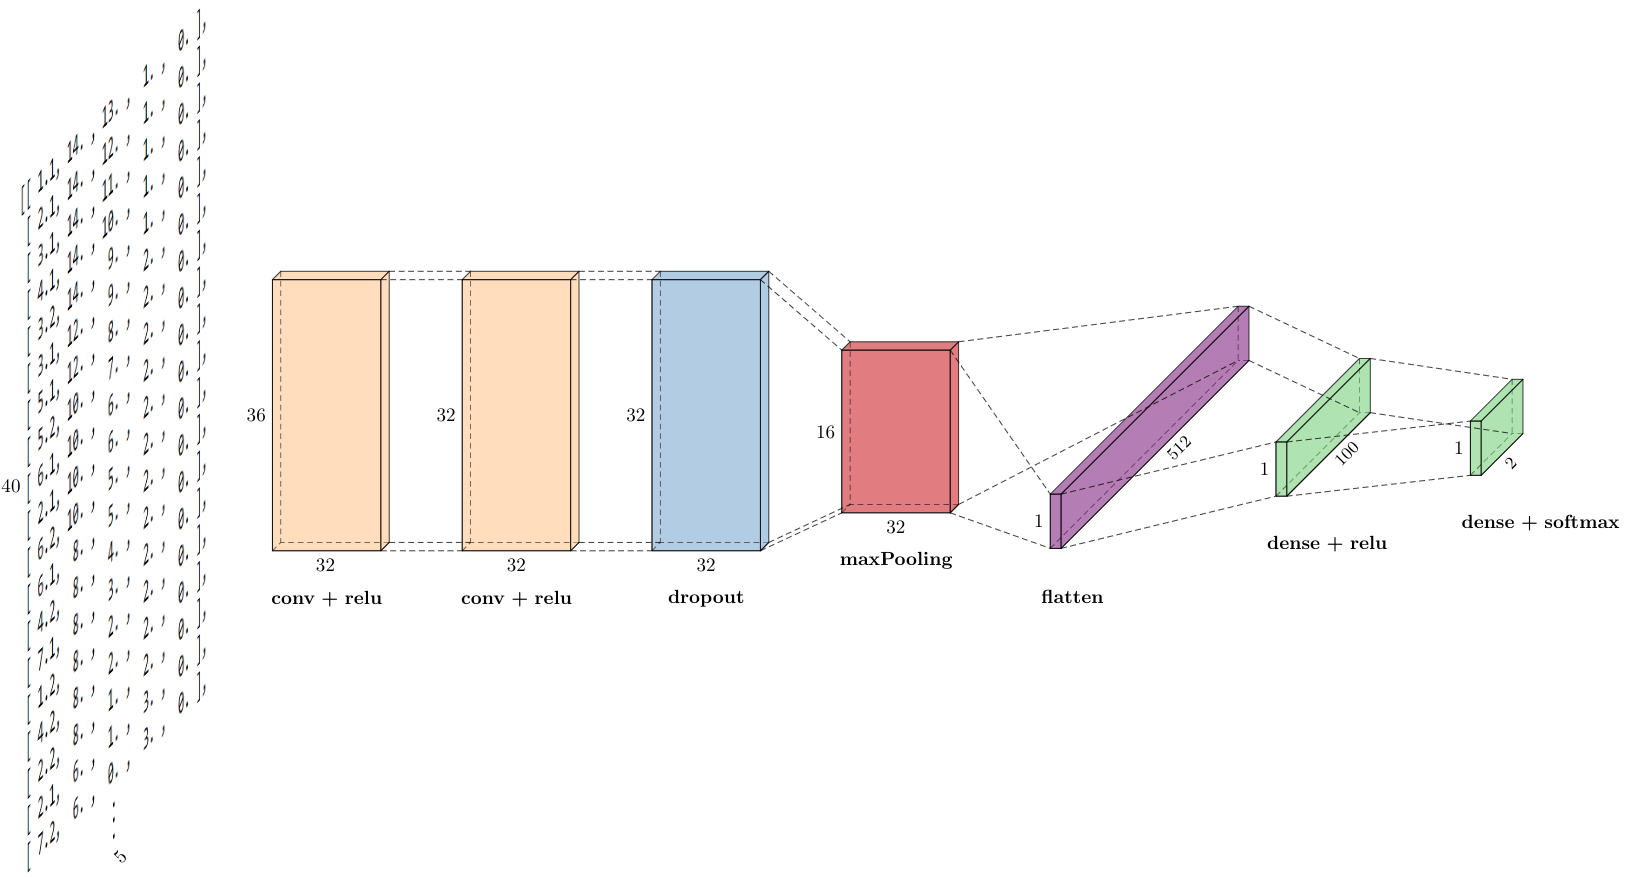
\includegraphics[width=15cm]{images/1dCnnStructureChanged.png}
	\caption[Visualization of the utilized 1D convnet topology.]{Visualization of the utilized 1D convnet topology. The dimensions represent those of the feature map in that layer. For example, the first convolution layer produces a feature map with the size 36 x 32 with 32 being the number of filters computed.\\ The input is on the left and the output on the right.}
	\label{fig:1dCnnStructure}
\end{figure}
The input data consist of the 5 statistical features, explained in section \ref{1d_cnn_features} \nameref{1d_cnn_features}, for each of the 40 steps (20 rounds), resulting in the input dimensions 40 x 5. Initially the data is passed to the first convolution layer of the network. The first layer computes 32 filters and the convolutional kernel has a size of 5, meaning that every step from the kernel includes all data from 5 steps in the game. The resulting feature map has a size of 36 x 32. This feature map is passed to the second convolution layer that computes the same number of filters. The kernel also has the same size like in the first layer. This results in a feature map with a size of 32 x 32. Afterwards, a dropout layer with a rate of 0.5 randomly sets input features to 0 to reduce overfitting. Then a one dimensional max-pooling layer with a pool size of 2 reduces the size of the feature map to 16 x 32. Afterwards, a flatten layer forms the features into one dimension. These features are finally passed to a densely connected network, consisting of two dense layers. Both convolution layers, and the first dense layer use a rectified linear unit as activation function. The last dense layer uses softmax as activation function to bring the data down to two values that specify the result of the classification. In total 57486 parameters are trained in this model. 

For the optimization, the Adam algorithm is used that is already implemented in Keras. Adam optimization is a stochastic gradient descent method \cite{keras}. The learning rate is set to 0.0001 and not changed during the training. The batch size is set to 32 and the model is trained for 2500 epochs. 
%Later many models had to be retrained due to complications and the epochs were reduced to 1500, because 2500 was unnecessarily high (accuracy continually decreased already after less than 1500 epochs).% As mentioned before, this is a best practice configuration

%As mentioned before, this is a best practice configuration, optimized over all the 1D convnet models and not individually for each model. 

\newpage

\subsection{2D convnet}
\label{2d_cnn}
The structure of the 2D convnet used is shown in figure \ref{fig:2dCnnStructure}.
\begin{figure}[H]
	\centering
	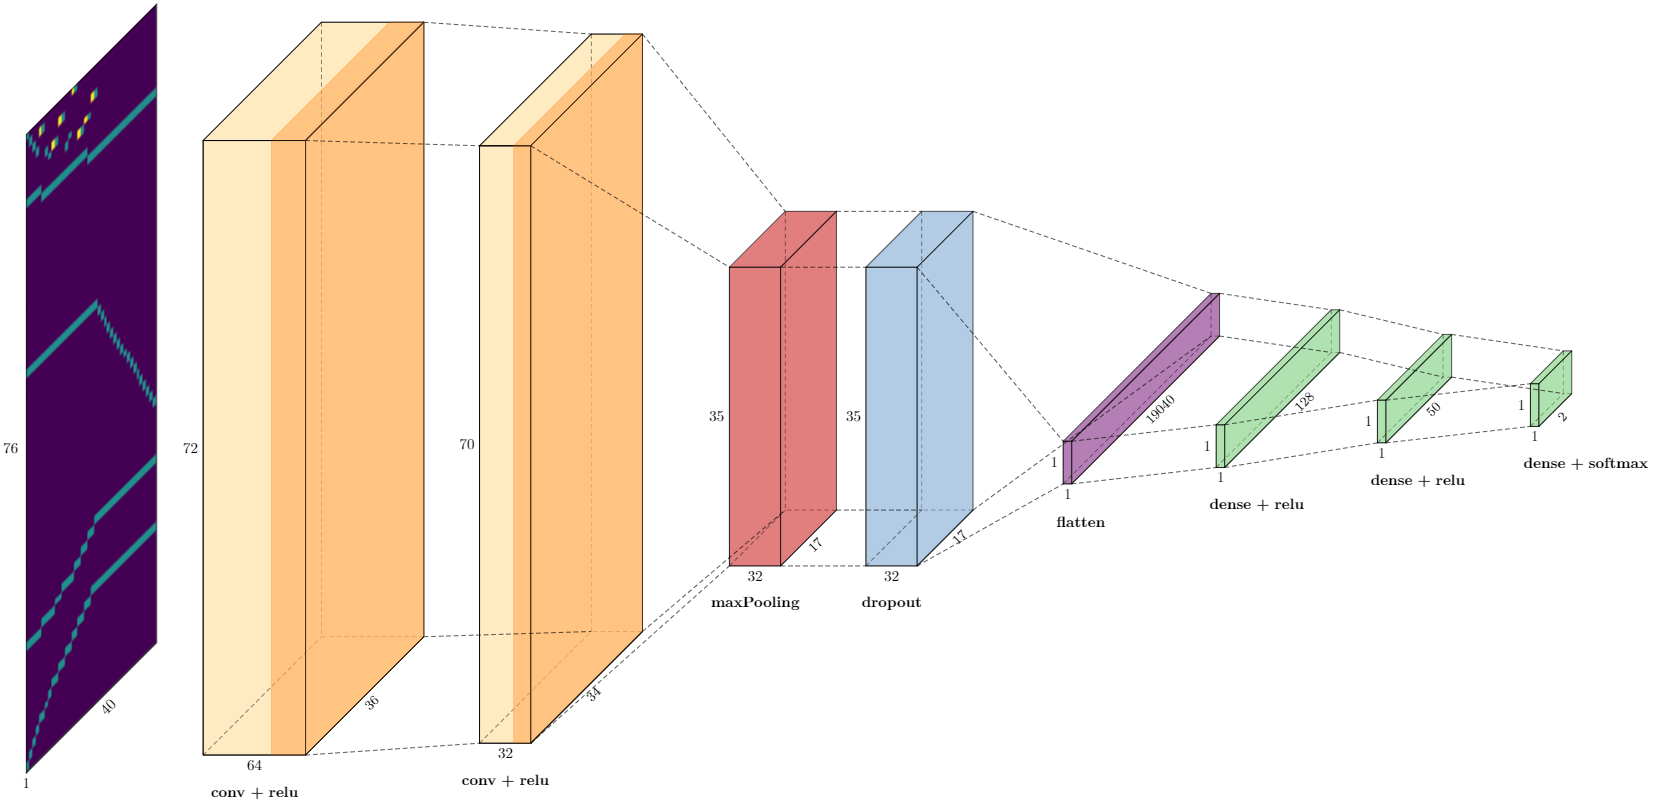
\includegraphics[width=15cm]{images/2dCnnStructure_new.png}
	\caption[Visualization of the utilized 2D convnet topology.]{Visualization of the utilized 2D convnet topology. The dimensions represent those of the feature map in that layer. For example, the first convolution layer produces a feature map with the size 72 x 36 x 64 with 64 describing the number of filters computed.\\ The input is on the left and the output on the right.}
	\label{fig:2dCnnStructure}
\end{figure}
The input data consist of the synthetic images generated in section \ref{2d_cnn_features} \nameref{2d_cnn_features}, using the 5 statistical features. This results in the input dimensions 76 x 40 x 1. Initially the data is passed to the first convolution layer of the network. It computes 64 filters and the convolutional kernel has a size of 5 x 5, meaning that each step from the kernel includes a 5 x 5 sized area of the synthetic image. This convolution results in a feature map with a size of 72 x 36 x 64. This feature map is passed to the second convolution layer that computes 32 filters with a kernel of size of 3 x 3. This results in a feature map with the size of 70 x 34 x 32. Then a two dimensional max pooling layer with a pool size of 2 x 2 reduces the size of the feature map to 35 x 17 x 32. Afterwards, a dropout layer with a rate of 0.2 randomly sets input units to 0 to reduce overfitting. Then a flatten layer forms the features into one dimension. These features are finally passed to a densely connected network, consisting of three dense layers. Both convolution layers, and the first two dense layers use a rectified linear unit as activation function. The last dense layer uses a softmax activation function to bring the data down to two values that specify the result of the classification. In total 2463928 parameters are trained in this model.

For the optimization, the Adam algorithm is used that is already implemented in Keras. Adam optimization is a stochastic gradient descent method \cite{keras}. The learning rate is set to 0.00001 and not changed during the training. The batch size is set to 32 and the model was initially trained for 500 epochs. Later, many 2D convnets had to be retrained due to complications and the epochs were reduced to 200, because 500 was unnecessarily high (accuracy continually decreased already after less than 500 epochs). This can be seen in figure \ref{fig:2d40}. 
% As mentioned before, this is a best practice configuration. 

%As mentioned before, this is a best practice configuration, optimized over all the 2D convnet models and not individually for each model. 

\begin{comment}

\subsubsection{Visualizing intermediate activations}
\todo{vielleichtz diese section rausnehemen. ich denke es ist unnötig, weil es nicht dazu beiträgt was meine arbeit zeigen soll}

An interesting thing about 2d cnns is that it is possible to vizualize the reprenestations learned by the network. This helps to understand the meaning of individual filters. Intermediate activations canm be vizualized by displaying the feauture maps that are the outpu of various convolution and pooling layers in the network, given an image is passed to the input layer. \todo{ref} To extract these feature maps, the model is first trained for one split and then run in prediction mode. Vizualizing each feature map produced by filters gives a view into how an input is decomposed into the different filters learned by the cnn. The decision was made not to focus too much on vizualizing all feature maps but instead to only vizualize one feature map created by each layer. As each feature map can learn different features, the following visualizations are only small fractions of what the cnn learns. Thgerefore they should only serve as exemplary illustration of what the different layers of the cnn output.

\todo{bisschen beschreiebn was was ist von den bildern und was man sieht}

\begin{minipage}{0.5\textwidth}
\begin{figure}[H]
\centering
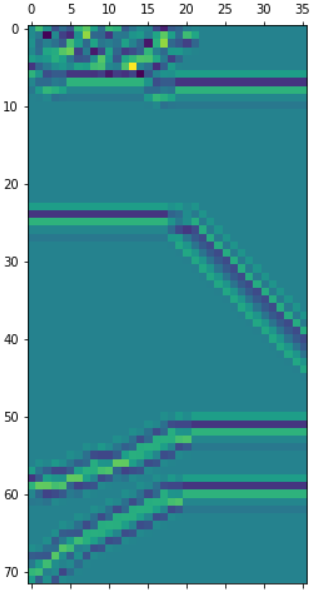
\includegraphics[width=5cm]{images/2dcnnLayer1.png}
\caption[Bild kurz]{Add caption}
\label{fig:vis2d1}
\end{figure}
\end{minipage}
\begin{minipage}{0.5\textwidth}
\begin{figure}[H]
\centering
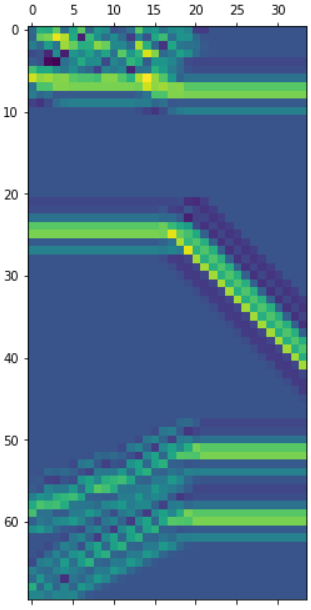
\includegraphics[width=5cm]{images/2dcnnLayer2.png}
\caption[Bild kurz]{Add caption}
\label{fig:vis2d2}
\end{figure}
\end{minipage}

\begin{minipage}{0.5\textwidth}
\begin{figure}[H]
\centering
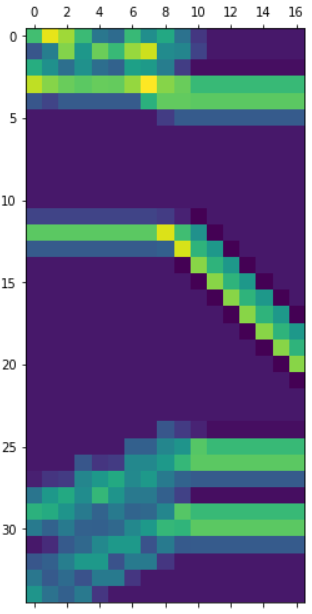
\includegraphics[width=5cm]{images/2dcnnLayer3.png}
\caption[Bild kurz]{Add caption}
\label{fig:vis2d3}
\end{figure}
\end{minipage}
\begin{minipage}{0.5\textwidth}
\begin{figure}[H]
\centering
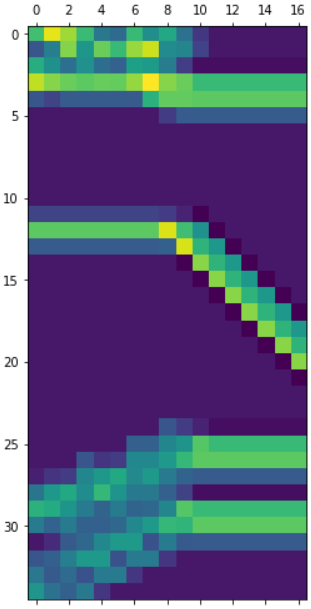
\includegraphics[width=5cm]{images/2dcnnLayer4.png}
\caption[Bild kurz]{Add caption}
\label{fig:vis2d4}
\end{figure}
\end{minipage}

It can be seen that the original structure of the image is still recognizable after all convolutional, pooling and dropout layers. When dealing with cnns that have more layers, usually the original image is at some point not recognizable anymore. The remaining layers of the 2d cnn effectively opperate on one dimensionaml data and create the output. Therfore they will be left out in this vizualization.


%Especially when dealing with more copmplex structures of cnns, vizualizing all feature maps instead of one, can reveal valuable informations. Generelly, the deeper the layer, the less of the original image is recogniazable. Since the size of the 2d cnn used is comparetively small, the original image is still recognizable after all convolutional, poolind and dropout layers.  For instance can be analysed if the structure of the cnn is overly complex for the data. This is the case if the last layers do not activate anymore, as there is nothing more to learn at that point, resulting in all values of the feature maps being 0. 


%If this technique is used for actually analysisng the cnn,  



%An interesting thing about 2d cnns, what is not possible to that extend in most of the neural networks, is that the steps in between can be vizualized. As each convolutional layer creates new images using the filters, it is actually possible to look at the images between layers. Generelly the deeper the layer the less from the actual image is recognizable. It can be observed how the network step by step forms the input image to the output shape. Although this is not especially usefull for actually knowing what the network does, it is usefull for knowing if certain layers of the network do something at all. If for instance the structure of the cnn is overly complex for the data, this will be indicated by the fact that the last layers are not activating at all becuase there is nothing more to learn at that point (all values of all feature maps from a layer are 0). Although the structure of the 2d cnn used is not very complex and this technique is more relevant for larger networks, it is interesting to exemplary look at the images between the convolutions of the 2d cnn used. To do so the model is first trained for one split and then run in predict mode. When passing an image to the imput layer it is then possible to extract the images between layers.

\todo{da wird ein buch erwähnt, wo der typ erzählt wieso es gut ist das zu machen. Die zitate umschreiben in meinen text: \url{https://towardsdatascience.com/visualizing-intermediate-activation-in-convolutional-neural-networks-with-keras-260b36d60d0}}

%... bild..

%As visible, there are no layers from which all filters do not activate, meaning the structure is not overly complex for the data. 

%\todo{referenz finden und bilder einbinden von dem 2d cnn. vielleicht auch ein bild von einem größeren netz wo es nichts mehr lernt.}

\end{comment}

\newpage

\section{Training setup}
\label{training_setup}
There is one script each for training the 1D convnet and the 2D convnet. The only differences are in the structure and the hyper parameters of the convnets and that before training the 2D convnet the loaded statistical features must first be used to create the synthetic images. Both scripts load the same statistical features, already divided into 20 splits that are used for leave-one-out cross validation. Each split contains a training and a test set. A training set consists of 19 real and 19000 simulated games for each of the two classes, while a test set contains one real game for each of the classes. The 2000 simulated games excluded from the training are not used for testing, because the results would not be representative of the real world performance of the models. Furthermore, only a certain number of the best simulations are included in the training. The ratio of n simulated games for each real games will be abbreviated with sdnx. For instance, sd5x means that 5 simulated games for each real game were included in the training. 
%As there are statistical features for 20 real and 20000 simulated no obstacles games as well as the same amount for glare effects games, this results in each split containing data from 19 real and 19000 simulated games for each of the two classes, resulting in 38 real and 38000 simulated games available for the training. From 2 real and 2000 simulated games not used for training, only the data from the real games is used for testing. \todo{leave one out cross validation erwähnen, generell umformulieren weil es maximal so viele simulierte sind und nicht generell} Testing on simulated data would not be representative of the real world performance of the models. Furthermore it can be chosen for which ratios between simulated and real games models should be trained. 
Each training of a model is done for the following ratios: sd0x, sd1x, sd2x, sd3x, sd4x, sd5x, sd6x, sd7x, sd8x, sd9x, sd10x and sd20x. Moreover, the training is done on different numbers of rounds (each round consists of flipping two cards). In real world scenarios, the less turns waited the faster the decision is made and assistance can be applied. However, if waited longer the decision will likely be correct more often. To analyse this, the models are trained each for 5, 10, 15 and 20 rounds. More than 20 turns were not recorded. As convnets are stochastic machine learning algorithms, different runs of the same algorithm on the same data can result in different outcomes. Therefore, it is not sufficient to train each model only once as the result is not reliable. Instead, the training of a model is repeated multiple times and the results are averaged to summarize the performance of the model \cite{repetition}. The decision was made to repeat the training of each model 20 times. 
% Training models for ranges of turns in the middle, for instance from turn 10 to 15, was left out, because this is not very interesting when conscidering real world usage. 

%All models are trained twice. Once on the simulated data created before modifying the simulator and once afterwards. This can potentially show whether the changes improved the classification results. 

%As mentioned in chapter \todo{ref}, the topology

%The structure and hyper parameters of the modells for all 1d cnns are identical. Same goes for all 2d models. The only differnece is the input shape of the modells since it depends on teh number of steps used in the training. Identical structure for modells of the same type are used so that different training results for different amount of steps can be reliably compared. It should be noted the structure and hyper paramters are not the same between the 1d and 2d cnns. 

Once one of the scripts is executed, required directory structures are created and training processes for the different ratios of real to simulated games are performed successively. The training for one ratio consists of parallelized training of 20 splits using multiprocessing. As the training for each split is repeated 20 times, for each ratio 20 models are created  for every split. This means that 400 models are trained for every ratio. As there are 12 different ratios trained, this results in 4800 models trained for each execution of one of the scripts. As mentioned above, the training is done for 4 different amounts of rounds for the 1D convnet and the 2D convnet. This adds up to 38400 models being trained. Furthermore, this is done twice: Once before the changes to the simulator and once afterwards, to see if the changes improved the performance of the models. All in all, this results in 76800 models. For each model the training history is saved in a file. Saving and loading the histories is necessary due to the parallel training of multiple models through multiprocessing. Once the training of the 4800 models of one script is completed, the training histories are loaded from the files. The results from the 400 training histories for each ratio of real to simulated games are averaged, plotted and the final figures are saved for the analysis.
% The reason for averaging the results over many models is, that deep neural networks by default initialize their weights randomly, resulting in potentially different outcomes of each training \todo{stattdessen begründung mit stochastic models mit referenz}. By averaging the results, the values and therefore the interpretation becomes more reliable and meaningful. 
All models are trained on the CPU. The fact that 76800 models are trained led to the decision, not to save all models but instead first evaluate the results and then retrain and save the models that create the best results thus using less memory.  

\begin{comment}


There are two main folders for storing the classification results. One for the results before the changes to the simulator and the other one for the results afterwards. Once one of the training scripts is executed, a subfolder for saving and loading 
The scripts create and use a specific directory structure conceptualized in figure \todo{ref}.
structure erklären

resutls -> 2d... -> sdxordner,(sdx images) -> split1 -> run1resutls 

\begin{tikzpicture}
[sibling distance=3cm,-,thick]
\footnotesize
\node {classification results}
child {node {modelType\_steps\_timestamp}
	[sibling distance=2cm]
	child {node {hi2.1}
		child {node {deciduous}}
		child {node {evergreen}}
	}
	child {node {...}}
	child {node {hi2.20}}
}
child {node {...}
}
child {node {...}
}
;
\end{tikzpicture}

\end{comment}

\newpage
   
\section{Training results and evaluation}
\label{training_results_and_evaluation}
The training results for the various configurations can be seen in table \ref{tab:1d_before}, \ref{tab:2d_before}, \ref{tab:1d_after} and \ref{tab:2d_after}. The first two tables contain the results before the changes to the simulator and the last two the results afterwards. The analysis will only focus on the accuracy, but the loss is also listed for the sake of completeness. The best accuracies for each number of turns in each table are highlighted in green. If multiple ratios of real to simulated games for a certain number of turns produce the same accuracy only the one with the smallest amount of simulations is highlighted. The accuracies in the tables are those from the best epochs. In most of the cases the models start overfitting after a certain epoch resulting in a deterioration of the accuracy after reaching a local maximum. In rare cases the test accuracy converges. Such a case can be observed in figure \ref{fig:1d20}.
%All models except the 1D convnet for 5 rounds and ratios of sd0x and sd1x reach such a local maximum in accuracy before the training is stopped. 

It should be clarified that the chosen configurations of models to be trained make no claim to completeness and do not claim to produce the best results, as they are not optimized individually. In all following tables the word round is abbreviated with r. and accuracy with acc. 


\newpage

\begin{comment}
	\begin{table}[H]
	\centering
	
	\resizebox{0.9\columnwidth}{!}{%
	\begin{tabular}{|c||ccccc|ccccc|ccccc|ccccc|}
	\hline
	&&& 5 r. &&&&& 10 r. &&&&& 15 r. &&&&& 20 r. &&\\
	\hline
	&& Acc. && Loss &&& Acc. && Loss &&& Acc. && Loss &&& Acc. && Loss &\\
	\hline\hline
	sd0x &&     65.12\% && 0.6584 &&& \textbf{\textcolor{mygreen}{81.12\%}} && 0.5116 &&& \textbf{\textcolor{mygreen}{78.37\%}} && 0.5377 &&& 79.62\% && 0.492 &\\
	sd1x &&     71.25\% && 0.6385 &&& 80.88\% && 0.4777 &&& 77.25\% && 0.5355 &&& 80.12\% && 0.4999 &\\
	sd2x &&     68.5\% && 0.6476 &&& 77.38\% && 0.5283 &&& 78.25\% && 0.5275 &&& \textbf{\textcolor{mygreen}{81.25\%}} && 0.4887 &\\
	sd3x &&     69.38\% && 0.6494 &&& 75.5\% && 0.5252 &&& 76.13\% && 0.5329 &&& 79.75\% && 0.4999 &\\
	sd4x &&     67.5\% && 0.6436 &&& 75.88\% && 0.538 &&& 77.25\% && 0.5322 &&& 81.25\% && 0.4975 &\\
	sd5x &&     72.25\% && 0.6212 &&& 76.5\% && 0.5252 &&& 77.75\% && 0.5338 &&& 81.25\% && 0.4985 &\\
	sd6x &&     71.87\% && 0.6346 &&& 74.75\% && 0.547 &&& 76.25\% && 0.5376 &&& 79.38\% && 0.5075 &\\
	sd7x &&     70.25\% && 0.6252 &&& 73.62\% && 0.5395 &&& 76.0\% && 0.5326 &&& 80.0\% && 0.5078 &\\
	sd8x &&     74.25\% && 0.6121 &&& 72.5\% && 0.5509 &&& 77.0\% && 0.535 &&& 79.75\% && 0.4993 &\\
	sd9x &&     \textbf{\textcolor{mygreen}{74.88\%}} && 0.5826 &&& 74.63\% && 0.5483 &&& 76.0\% && 0.542 &&& 81.75\% && 0.4987 &\\
	sd10x &&    74.87\% && 0.5971 &&& 74.5\% && 0.5558 &&& 77.12\% && 0.5394 &&& 80.87\% && 0.5036 &\\
	sd20x &&    73.25\% && 0.5831 &&& 73.5\% && 0.5493 &&& 75.63\% && 0.5355 &&& 80.75\% && 0.5013 &\\
	\hline
	\end{tabular}
	}
	\caption[Best accuracies and losses produced by the 1D convnet. Before the changes to the simulator.]{Best accuracies and losses for 5, 10, 15 and 20 rounds produced by the 1D convnet. Before the changes to the simulator.}
	\label{tab:1d_before_old}
	\end{table}
\end{comment}

\begin{table}[H]
	\centering
	
	\resizebox{0.9\columnwidth}{!}{%
		\begin{tabular}{|c||ccccc|ccccc|ccccc|ccccc|}
			\hline
			&&& 5 r. &&&&& 10 r. &&&&& 15 r. &&&&& 20 r. &&\\
			\hline
			&& Acc. && Loss &&& Acc. && Loss &&& Acc. && Loss &&& Acc. && Loss &\\
			\hline\hline
			sd0x &&     65.12\% && 0.6584 &&& \textbf{\textcolor{mygreen}{81.88\%}} && 0.507 &&& \textbf{\textcolor{mygreen}{78.63\%}} && 0.5415 &&& 78.75\% && 0.5039 &\\
			sd1x &&     71.25\% && 0.6385 &&& 81.75\% && 0.4899 &&& 77.38\% && 0.5399 &&& 80.62\% && 0.4893 &\\
			sd2x &&     68.5\% && 0.6476 &&& 77.38\% && 0.5128 &&& 77.25\% && 0.539 &&& 80.0\% && 0.4965 &\\
			sd3x &&     69.38\% && 0.6494 &&& 77.5\% && 0.5135 &&& 75.75\% && 0.5364 &&& 79.88\% && 0.4928 &\\
			sd4x &&     67.5\% && 0.6436 &&& 77.5\% && 0.5446 &&& 76.13\% && 0.5418 &&& \textbf{\textcolor{mygreen}{81.12\%}} && 0.501 &\\
			sd5x &&     72.25\% && 0.6212 &&& 74.5\% && 0.5404 &&& 78.25\% && 0.5286 &&& 81.0\% && 0.5005 &\\
			sd6x &&     71.87\% && 0.6346 &&& 75.25\% && 0.5412 &&& 77.12\% && 0.5356 &&& 80.25\% && 0.4967 &\\
			sd7x &&     70.25\% && 0.6252 &&& 73.38\% && 0.5453 &&& 75.63\% && 0.5357 &&& 81.12\% && 0.4918 &\\
			sd8x &&     74.25\% && 0.6121 &&& 73.38\% && 0.5486 &&& 77.0\% && 0.5316 &&& 80.38\% && 0.5036 &\\
			sd9x &&     \textbf{\textcolor{mygreen}{74.88\%}} && 0.5826 &&& 74.25\% && 0.5369 &&& 76.5\% && 0.5408 &&& 80.25\% && 0.4909 &\\
			sd10x &&    74.87\% && 0.5971 &&& 76.38\% && 0.5594 &&& 76.25\% && 0.548 &&& 80.25\% && 0.501 &\\
			sd20x &&    73.25\% && 0.5831 &&& 73.25\% && 0.5414 &&& 76.0\% && 0.5387 &&& 80.87\% && 0.4935 &\\
			\hline
		\end{tabular}
	}
	\caption[Best accuracies and losses produced by the 1D convnet, prior to the changes to the simulator.]{Best accuracies and losses for 5, 10, 15 and 20 rounds produced by the 1D convnet, prior to the changes to the simulator.}
	\label{tab:1d_before}
\end{table}

\begin{table}[H]
	\centering
	
	\resizebox{0.9\columnwidth}{!}{%
	\begin{tabular}{|c||ccccc|ccccc|ccccc|ccccc|}
		\hline
		&&& 5 r. &&&&& 10 r. &&&&& 15 r. &&&&& 20 r. &&\\
		\hline
		&& Acc. && Loss &&& Acc. && Loss &&& Acc. && Loss &&& Acc. && Loss &\\
		\hline\hline
		sd0x &&     63.5\% && 0.6471 &&& 74.0\% && 0.4991 &&& 79.62\% && 0.4726 &&& 79.0\% && 0.4778 &\\
		sd1x &&     68.12\% && 0.619 &&& 76.62\% && 0.5171 &&& 79.5\% && 0.4984 &&& 81.75\% && 0.4735 &\\
		sd2x &&     68.25\% && 0.6382 &&& \textbf{\textcolor{mygreen}{80.0\%}} && 0.5243 &&& 80.38\% && 0.4851 &&& 84.12\% && 0.4573 &\\
		sd3x &&     69.5\% && 0.6392 &&& 78.88\% && 0.5518 &&& 80.25\% && 0.5038 &&& 84.62\% && 0.4718 &\\
		sd4x &&     67.63\% && 0.6415 &&& 76.38\% && 0.5685 &&& 79.62\% && 0.5106 &&& \textbf{\textcolor{mygreen}{85.0\%}} && 0.4726 &\\
		sd5x &&     70.88\% && 0.6339 &&& 74.63\% && 0.5668 &&& 80.0\% && 0.51 &&& 84.88\% && 0.474 &\\
		sd6x &&     70.62\% && 0.638 &&& 77.0\% && 0.5623 &&& 80.12\% && 0.5077 &&& 84.88\% && 0.4776 &\\
		sd7x &&     69.75\% && 0.6543 &&& 75.38\% && 0.5762 &&& 79.5\% && 0.5176 &&& 85.0\% && 0.4839 &\\
		sd8x &&     70.0\% && 0.6467 &&& 74.25\% && 0.5775 &&& 80.38\% && 0.5164 &&& 85.0\% && 0.484 &\\
		sd9x &&     71.25\% && 0.6395 &&& 78.75\% && 0.5696 &&& \textbf{\textcolor{mygreen}{81.5\%}} && 0.5064 &&& 85.0\% && 0.4814 &\\
		sd10x &&    68.75\% && 0.6296 &&& 77.75\% && 0.5674 &&& 80.12\% && 0.5098 &&& 85.0\% && 0.4802 &\\
		sd20x &&    \textbf{\textcolor{mygreen}{73.0\%}} && 0.5833 &&& 76.63\% && 0.5486 &&& 79.75\% && 0.5064 &&& 84.88\% && 04704 &\\
		\hline
	\end{tabular}
	}
	\caption[Best accuracies and losses produced by the 2D convnet, prior to the changes to the simulator.]{Best accuracies and losses for 5, 10, 15 and 20 rounds produced by the 2D convnet, prior to the changes to the simulator.}
	\label{tab:2d_before}
\end{table}

\begin{table}[H]
	\centering
	
	\resizebox{0.9\columnwidth}{!}{%
		\begin{tabular}{|c||ccccc|ccccc|ccccc|ccccc|}
			\hline
			 &&& 5 r. &&&&& 10 r. &&&&& 15 r. &&&&& 20 r. &&\\
			\hline
			 && Acc. && Loss &&& Acc. && Loss &&& Acc. && Loss &&& Acc. && Loss &\\
			\hline\hline
			sd0x &&     63.87\% && 0.6698 &&& \textbf{\textcolor{mygreen}{81.88\%}} && 0.5014 &&& 78.5\% && 0.5401 &&& 78.62\% && 0.5107 &\\
			sd1x &&     67.75\% && 0.6648 &&& 79.0\% && 0.5095 &&& 75.75\% && 0.5305 &&& 79.38\% && 0.5101 &\\
			sd2x &&     66.0\% && 0.6506 &&& 79.25\% && 0.4845 &&& 76.0\% && 0.5325 &&& 78.37\% && 0.514 &\\
			sd3x &&     64.38\% && 0.6585 &&& 77.38\% && 0.5037 &&& 77.62\% && 0.5261 &&& 79.25\% && 0.5113 &\\
			sd4x &&     67.0\% && 0.6377 &&& 75.38\% && 0.5289 &&& 77.62\% && 0.5331 &&& \textbf{\textcolor{mygreen}{80.25\%}} && 0.5027 &\\
			sd5x &&     67.0\% && 0.6452 &&& 76.75\% && 0.5146 &&& \textbf{\textcolor{mygreen}{78.75\%}} && 0.5226 &&& 79.0 && 0.5042 &\\
			sd6x &&     70.25\% && 0.6427 &&& 75.25\% && 0.5335 &&& 78.75\% && 0.5208 &&& 79.38\% && 0.5049 &\\
			sd7x &&     70.25\% && 0.6449 &&& 76.88\% && 0.5114 &&& 78.0\% && 0.5129 &&& 78.75\% && 0.5115 &\\
			sd8x &&     71\% && 0.628 &&& 76.25\% && 0.523 &&& 77.25\% && 0.5261 &&& 79.12\% && 0.5156 &\\
			sd9x &&     70\% && 0.6276 &&& 75.37\% && 0.5226 &&& 77.62\% && 0.5281 &&& 78.63\% && 0.522 &\\
			sd10x &&    71.5\% && 0.6242 &&& 76.25\% && 0.5261 &&& 76.38\% && 0.5331 &&& 78.62\% && 0.4986 &\\
			sd20x &&    \textbf{\textcolor{mygreen}{71.88\%}} && 0.6246 &&& 72.38\% && 0.5617 &&& 76.25\% && 0.5416 &&& 79.12\% && 0.5 &\\
			\hline
		\end{tabular}
	}
	\caption[Best accuracies and losses produced by the 1D convnet, after the changes to the simulator.]{Best accuracies and losses for 5, 10, 15 and 20 rounds produced by the 1D convnet, after the changes to the simulator.}
	\label{tab:1d_after}
\end{table}

\begin{table}[H]
	\centering

	\resizebox{0.9\columnwidth}{!}{%
		\begin{tabular}{|c||ccccc|ccccc|ccccc|ccccc|}
			\hline
			&&& 5 r. &&&&& 10 r. &&&&& 15 r. &&&&& 20 r. &&\\
			\hline
			&& Acc. && Loss &&& Acc. && Loss &&& Acc. && Loss &&& Acc. && Loss &\\
			\hline\hline
			sd0x &&     63.62\% && 0.6461 &&& 73.87\% && 0.4929 &&& 80.0\% && 0.4557 &&& 78.5\% && 0.476 &\\
			sd1x &&     67.88\% && 0.6446 &&& 76.12\% && 0.531 &&& 79.5\% && 0.4911 &&& 79.75\% && 0.4874 &\\
			sd2x &&     69.75\% && 0.6463 &&& \textbf{\textcolor{mygreen}{79.62\%}} && 0.5243 &&& 80.87\% && 0.4905 &&& \textbf{\textcolor{mygreen}{80.0\%}} && 0.4859 &\\
			sd3x &&     69.5\% && 0.6449 &&& 77.5\% && 0.5507 &&& \textbf{\textcolor{mygreen}{82.25\%}} && 0.4994 &&& 80.0\% && 0.4865 &\\
			sd4x &&     69.0\% && 0.6347 &&& 72.75\% && 0.5684 &&& 80.12\% && 0.5156 &&& 80.0\% && 0.495 &\\
			sd5x &&     69.38\% && 0.6342 &&& 73.62\% && 0.5634 &&& 80.5\% && 0.5122 &&& 80.0\% && 0.4917 &\\
			sd6x &&     \textbf{\textcolor{mygreen}{71.0\%}} && 0.6326 &&& 74.5\% && 0.5586 &&& 80.62\% && 0.5038 &&& 79.5\% && 0.4874 &\\
			sd7x &&     70.0\% && 0.6328 &&& 71.62\% && 0.555 &&& 80.0\% && 0.5061 &&& 79.5\% && 0.4874 &\\
			sd8x &&     69.88\% && 0.6287 &&& 72.75\% && 0.5567 &&& 80.25\% && 0.5057 &&& 79.62\% && 0.4874 &\\
			sd9x &&     69.12\% && 0.6238 &&& 72.38\% && 0.5532 &&& 79.5\% && 0.5067 &&& 78.88\% && 0.4887 &\\
			sd10x &&    69.5\% && 0.6203 &&& 73.25\% && 0.5536 &&& 79.5\% && 0.5062 &&& 79.0\% && 0.4904 &\\
			sd20x &&    69.88\% && 0.5935 &&& 73.0\% && 0.5494 &&& 79.62\% && 0.5005 &&& 78.75\% && 0.4874 &\\
			\hline
		\end{tabular}
	}
	\caption[Best accuracies and losses produced by the 2D convnet, after the changes to the simulator.]{Best accuracies and losses for 5, 10, 15 and 20 rounds produced by the 2D convnet, after the changes to the simulator.}
	\label{tab:2d_after}
\end{table}

\newpage

\begin{comment}



\begin{table}[H]
	\centering
	\caption{2D CNN. best accuracys for 5, 10, 15 and 20 steps. in brackets behind the accuiracy is the epoch.}%\label{tab1}
	\begin{tabular}{|l|l|l|l|l|}
		\hline
		Simulated Games & 5 steps & 10 steps & 15 steps& 20 steps\\
		\hline
		0 &   & && \\
		1 &  & && \\
		2 &  & && \\
		3 &  & && \\
		4 &  & && \\
		5 & &&& \\
		6 &  & && \\
		7 &  & && \\
		8 &  & && \\
		9 &  & && \\
		10 & &&& \\
		20 & &&& \\
		\hline
	\end{tabular}
\end{table}

\begin{table}[H]
	\centering
	\caption{1D CNN. best accuracys for 5, 10, 15 and 20 steps. in brackets behind the accuiracy is the epoch.}%\label{tab1}
	\begin{tabular}{|l|l|l|l|l|}
		\hline
		Simulated Games & 5 steps & 10 steps & 15 steps& 20 steps\\
		\hline
		0 &   & && \\
		1 &  & && \\
		2 &  & && \\
		3 &  & && \\
		4 &  & && \\
		5 & &&& \\
		6 &  & && \\
		7 &  & && \\
		8 &  & && \\
		9 &  & && \\
		10 & &&& \\
		20 & &&& \\
		\hline
	\end{tabular}
\end{table}

\begin{table}[H]
	\centering
	\caption{2D CNN. 20 turns. config2}%\label{tab1}
	\begin{tabular}{|l|l|l|}
		\hline
		Simulated Games & Best Accuracy (Epoch) & Best Loss (Epoch)\\
		\hline
		0 & 0.7888 (14) & 0.4822 (51) \\
		1 &  &  \\
		2 &  &  \\
		3 &  &  \\
		4 &  &  \\
		5 & 0.8450 (17) & 0.4768 (20) \\
		6 &  &  \\
		7 &  &  \\
		8 &  &  \\
		9 &  &  \\
		10 & 0.8475 (20) & 0.4796 (10) \\
		20 & 0.8437 (6) & 0.4763 (6) \\
		\hline
	\end{tabular}
\end{table}

- 1d cnn können besser mit kurzen sequencen umgehen als 2d. aber 2d sind bei mehr schritten deutlsich besser. (erste einschätzung) 

\begin{table}[H]
	\centering
	\caption{2D CNN. 20 turns. config1}%\label{tab1}
	\begin{tabular}{|l|l|l|}
		\hline
		Simulated Games & Best Accuracy (Epoch) & Best Loss (Epoch)\\
		\hline
		0 & 0.7963 (18) & 0.4931 (98) \\
		1 &  &  \\
		2 &  &  \\
		3 &  &  \\
		4 &  &  \\
		5 & 0.8437 (53) & 0.4821 (31) \\
		6 &  &  \\
		7 &  &  \\
		8 &  &  \\
		9 &  &  \\
		10 &  &  \\
		20 &  &  \\
		\hline
	\end{tabular}
\end{table}

\end{comment}

%- \todo{ich könnte noch plots machen die verlauf entwerder mit festen sd und unterschiedlicher anzahl rounds oder mit feaster rounds und unterscheidlichem sd zeigen. Nicht muss aber wäre cool, falls es sinnvoll ist. Muss ich nochmal gucken. Vielleicht an einem beispeiel um zu zeigen dass es von vorteil sein kann simulierte daten mit zu benutzen in unserem fall}

%- interessant: 1d cnn 5 rounds gucken ob sich der trend weiter führt und sogar noch besser wird

The results show that using a certain number of simulated games for the training can often significantly improve the classification results over using only the real data. A good example is the accuracy for sd0x compared to sd4x for 20 rounds for the 2D convnet in table \ref{tab:2d_before}. Using no simulations the accuracy is 79.0\% while for a ratio of 4 simulations for each real game the accuracy is 85.0\%. Furthermore, it can be seen that using too many simulations compared to real games can decrease the accuracy. In table \ref{tab:2d_before}, for 10 rounds, the accuracy for sd2x is 80.0\% and less when using more simulations. This behaviour highly varies depending on the configuration of the model. Sometimes the models produce the best results without any simulations, while other times using simulations strongly outperforms using only real data. It is possible that the optimal ratios of simulated to real games are not included the tested configurations. Especially the 2D convnet for 5 rounds before the changes to the simulator achieves its best accuracy with the highest ratio that was tested. Therefore, the optimal ratio could be higher than 20 simulations for each real game. 

\begin{minipage}[c]{0.4\textwidth}
	When looking at the best accuracies of 1D and 2D convnets for each number of rounds, it can be observed, that the best accuracies of the 1D convnets are lower on 15 and 20 rounds than on 10, while this is not the case for 2D convnets. This can be seen in figure \ref{fig:bestAccPlot}. The fact that the 1D convnets do not profit from more than 10 rounds might be related to the findings from section \ref{evaluation_of_simulation} \nameref{evaluation_of_simulation}, which indicate that the simulator performs worse in later rounds.
\end{minipage}
\begin{minipage}[c]{0.6\textwidth}
	\begin{figure}[H]
		\centering
		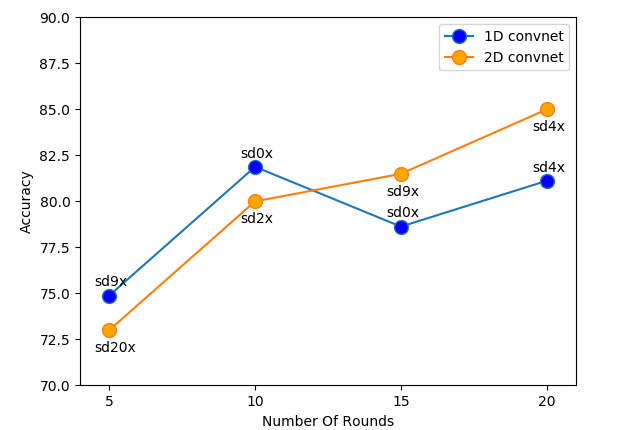
\includegraphics[width=9.8cm]{images/bestAccPlotNew.png}
		\caption[Best results for the different number of rounds before the changes to the simulator.]{Best results for the different number\\\hspace{0\textheight} of rounds before the changes to the simulator. Ratios\\\hspace{0\textheight} of real to simulated games is additionally described.}
		\label{fig:bestAccPlot}
	\end{figure}
\end{minipage}

 However, if the case, this begs the questions why this does not apply to 2D convnets. There is a possibility that the worse performance in later turns has a strong impact on the statistical features fed to the 1D convnet, but once these features are used to create the synthetic images for the 2D convnet this negative impact decreases. Figure \ref{fig:bestAccPlot} additionally shows the ratios of simulated to real data for each of the best results. The fact that the 2D convnets for 15 rounds have the best results when using 9 simulated games for each real game while the best configurations of the 1D convnets for 15 rounds use no simulations, supports the theory from above. Nonetheless the findings are not sufficient to verify the theory. For that more research would be required. However, if found to be true, it could mean that 2D convnets using synthetic images have the potential to handle inaccurate simulations better than 1D convnets. From a different perspective, this could also indicate that, assuming the simulator does actually perform worse in later rounds and is improved in that regard, the accuracy of the 1D convnets after 10 rounds could be improved.


\newpage


%beobachtung: bei 2d sind simulationen länger besser. Analysieren ob es daran liegt dass die anderen keine convergence erreichen. Wenn nicht dann ist es coole entdckung. Weil es ein anzeichen dafür ist, dass die 2d cnn besser mit simulationen lernen kann als 1d cnn. This also fits to the observation, that the results from 1dcnn with more than 10 rounds dont get much better if not worse. This can be caused by the fact that the simulations are less accurate after the first 10 steps, and therefore the 1d cnn does not improve by including them. However, the 2d cnn does improve using the last steps. This is an additional indicator, that the 2d cnn can better handle simulated games. A possibility is, that the difernce between simualted and real games in the synthetic images created using the feautre is not as siificant as when direclty using the statistical features in the 1d cnn. \todo{noch mit zahlen aus den tabelen begründen. und sagen dass die alle convergence erreichen, weshalb man das sagen kann}

% easy to believe that in some cases more the optimal ratio has not been reached yet, if only looking at the tables. However there are more factors that influnece the result. This becomes evident when plotting the trainig histories for accuracy and loss. ... plott wo wan sieht das divergence nicht erreicht wurde... The fact that the trainings with a lower ratio result in worse accuracy dont neccessarily are caused by the fact that more simulated games would be better, but could also be influenced by the fact that the divergence has not been reache yet, meaning that either a different learning rate or more epochs could increase the accuray. Therefore it can not be said with certainty that ore simulated games would in that case lead to the optimal result, as the optimal result could also be with less simulated but with changed hyper parameters. However, the hyper paramaters were intentinally chossen the same so that the results could be compared with each other.
 
It was considered to perform statistical tests comparing different models and ratios to reveal significant or insignificant differences. However, the decision was made that this does not really give reliable results, because the results are not necessarily the best achievable as the models were not individually optimized. Therefore, the results of statistical tests performed on the achieved accuracies, would not justify any statements regarding whether 1D convnets or 2D convnets perform significantly better. Such statistical tests would only show significant differences or indifferences in the results, but could not be interpreted for any valuable findings, as not all models are used to their full potential. For choosing the best configurations from those tested no statistical tests are used. Instead simply those with the highest accuracies are chosen.

%If hyper paremeters such as the leraning rate or the number of epochs are not chosen equal accross all models of one tabel (menaing all models for 1d cnns, etc) and instead would be chosen more indivuidually to optimize the models specifically for each number of rounds and ratoin between simuated and real games, the accuracie could be signifcantly different. Additionally the topologies of all models of one type are chosen the same, although this might not produce the best results for each configuration.

\begin{table}[H]
	\centering
	
	\resizebox{\columnwidth}{!}{%
		\begin{tabular}{|l||c|c|c|c|c|}
			\hline
			 & 5 r. & 10 r. & 15 r. & 20 r. & Average  \\
			\hline
			\hline
			1D convnet - before & 74.88\% (sd9x) & 81.88\% (sd0x) &78.63\% (sd0x) & 81.12\% (sd4x) & 79.13\% \\
			1D convnet - afterwards& 71.88\% (sd20x) & 81.88\% (sd0x) &78.75\% (sd5x) & 80.25\% (sd4x)  & 78.19\%  \\
			\hline
			2D convnet - before & 73.0\% (sd20x) & 80.0\% (sd2x) &81.5\% (sd9x) & 85.0\% (sd4x)  & 79.88\% \\
			2D convnet - afterwards & 71.0\% (sd6x) & 79.62\% (sd2x) & 82.25\% (sd3x) & 80.0\% (sd2x) & 78.22\% \\
			\hline
		\end{tabular}
	}
	\caption[Highest accuracies before and after the changes to the simulator.]{Highest accuracies before and after the changes to the simulator. Furthermore, the rations of simulated to real games and the average accuracies of the best results from each configuration are shown.}
	\label{tab:best_acc}
\end{table}

Table \ref{tab:best_acc} shows the best result for all categories before and after changing the simulator. It can be seen that although some accuracies are slightly better after the changes to the simulator the results are on average noticeably worse than before. The accuracy from the 2D convnet for 20 rounds, for instance, is decreased from 85.0\% to 80.0\%. The reason for this is unknown and can be highly complex, due to the many factors involved. A theory is, that reducing the randomness of the simulator and therefore making the simulated games more similar to the real games, may have resulted in a decreased generalising ability of the models and therefore less robustness on unknown data. However, this theory can hardly be verified. The overall decreased performance after the changes leads to the decision to only use the models trained on the simulated data created before the changes to the simulator. The chosen configurations for the different numbers of rounds can be seen in table \ref{tab:chosen_configs}. 

\begin{table}[H]
	\centering
	
		\begin{tabular}{|l||c|c|c|c|}
			\hline
			& 5 r. & 10 r. & 15 r. & 20 r.  \\
			\hline
			\hline
			1D convnet & 74.88\% (sd9x) & 81.88\% (sd0x) & &  \\
			\hline
			2D convnet &  & & 81.5\% (sd9x) & 85.0\% (sd4x)  \\
			\hline
		\end{tabular}
	\caption[The chosen configurations and their accuracies.]{The chosen configurations and their accuracies (averaged over 400 models each). }%\label{tab1}
	\label{tab:chosen_configs}
\end{table}

The 1D convnets trained, perform better for 5 and 10 rounds than 2D convnets, while 2D convnets perform better for 15 and 12 rounds. Depending on the number of rounds it can therefore be beneficial to use either 1D convnets or 2D convnets. The 4 best configurations for the different numbers of rounds are used in section \ref{voting} \nameref{voting}. Figures \ref{fig:1d10}, \ref{fig:1d20}, \ref{fig:2d30} and \ref{fig:2d40} show the average training and test accuracy during the course of training the models of these 4 configurations. 

\begin{minipage}{0.5\textwidth}
	\begin{figure}[H]
		\centering
		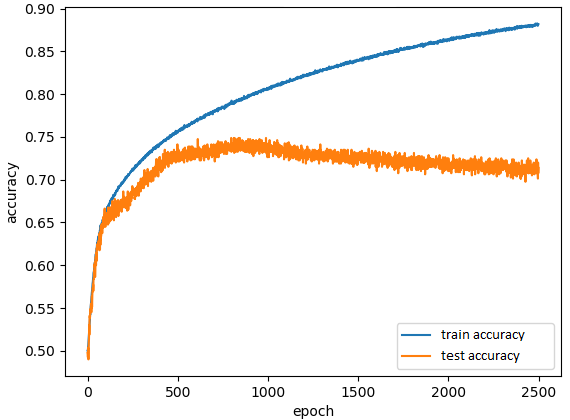
\includegraphics[width=7.5cm]{images/bestHistories/edit/1d_10s_sd9x_acc.png}
		\caption[Average training and test accuracy of 400 1D convnets on 5 rounds and a ratio of 9 simulated games for each real game.]{Average training and \\\hspace{0\textwidth}test accuracy of 400 1D convnets \\\hspace{0\textwidth}on 5 rounds and a ratio of 9 simulated  \\\hspace{0\textwidth}games for each real game. Best test \\\hspace{0\textwidth}accuracy is 74.88\% at epoch 812.}
		\label{fig:1d10}
	\end{figure}
\end{minipage}
\begin{minipage}{0.5\textwidth}
	\begin{figure}[H]
		\centering
		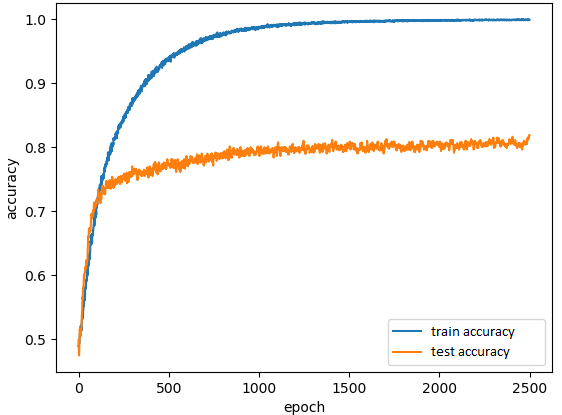
\includegraphics[width=7.5cm]{images/bestHistories/edit/1d_20s_sd0x_acc_new.png}
		\caption[Average training and test accuracy of 400 1D convnets on 10 rounds using no simulated games.]{Average training and \\\hspace{0\textwidth}test accuracy of 400 1D convnets \\\hspace{0\textwidth}on 10 rounds using no simulated \\\hspace{0\textwidth}games. Best test accuracy\\\hspace{0\textwidth} is 81.88\% at epoch 2498.}
		%\caption[Bild kurz]{Training history of 1d cnn\\\hspace{0\textwidth} on 10 rounds and using no  \\\hspace{0\textwidth} simulated games. Best validation \\\hspace{0\textwidth}accuracy is 81.12\% at epoch 1317.}
		\label{fig:1d20}
	\end{figure}
\end{minipage}

\begin{minipage}{0.5\textwidth}
	\begin{figure}[H]
		\centering
		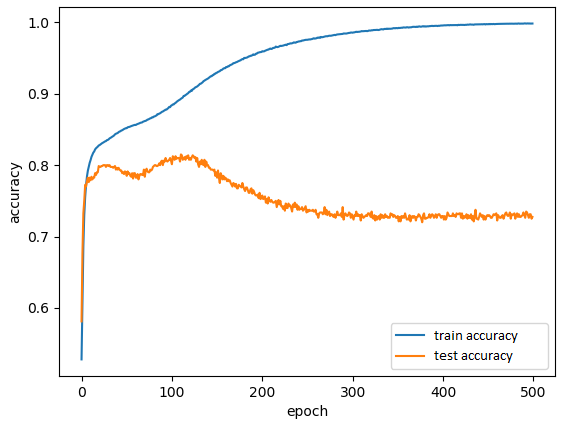
\includegraphics[width=7.5cm]{images/bestHistories/edit/2d_30s_sd9x_acc.png}
		\caption[Average training and test accuracy of 400 2D convnets on 15 rounds and a ratio of 9 simulated games for each real game.]{Average training and \\\hspace{0\textwidth}test accuracy of 400 2D convnets \\\hspace{0\textwidth}on 15 rounds and a ratio of 9 simulated  \\\hspace{0\textwidth}games for each real game. Best test \\\hspace{0\textwidth}accuracy is 81.5\% at epoch 111.}
		%\caption[Bild kurz]{Training history of 2d cnn\\\hspace{0\textwidth} on 10 rounds and a ratio of 9 simulated  \\\hspace{0\textwidth}games for each real game. Best validation \\\hspace{0\textwidth}accuracy is 74.88\% at epoch 812.}
		%\caption[Bild kurz]{best validation \\\hspace{0\textwidth}accuracy 81.5\% (at epoch 111)}
		\label{fig:2d30}
	\end{figure}
\end{minipage}
\begin{minipage}{0.5\textwidth}
	\begin{figure}[H]
		\centering
		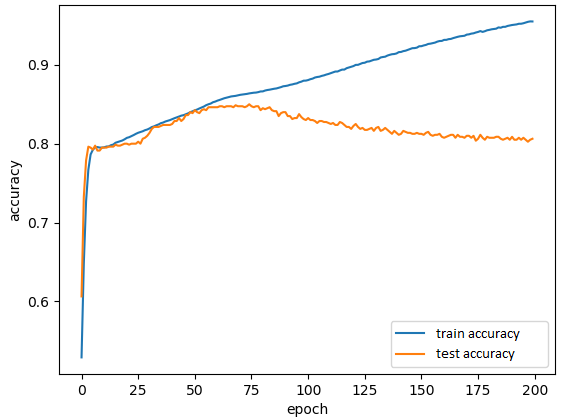
\includegraphics[width=7.5cm]{images/bestHistories/edit/2d_40s_sd4x_acc.png}
		\caption[Average training and test accuracy of 400 2D convnets on 20 rounds and a ratio of 4 simulated games for each real game.]{Average training and \\\hspace{0\textwidth}test accuracy of 400 2D convnets \\\hspace{0\textwidth}on 20 rounds and a ratio of 4 simulated \\\hspace{0\textwidth}games for each real game. Best test \\\hspace{0\textwidth}accuracy is 85.0\% at epoch 75.}
		%\caption[Bild kurz]{Training history of 1d cnn\\\hspace{0\textwidth} on 10 rounds and a ratio of 9 simulated  \\\hspace{0\textwidth}games for each real game. Best validation \\\hspace{0\textwidth}accuracy is 74.88\% at epoch 812.}
		%\caption[Bild kurz]{best validation \\\hspace{0\textwidth}accuracy 85.0\% (at epoch 75)}
		\label{fig:2d40}
	\end{figure}
\end{minipage}

%Due to complications many configurations had to be retrained. As it was known from prior tests that certain configurations do not improve after a certain number of epochs and due to the time constraints of this work the models were retrained with not as many epochs to save time. For instant the test accuracies of the 2D convnets trained on 20 rounds do not improve any more after around 60 or 70 epochs and therefore the retraining of the models was only done on 200 epochs as shown in figure \ref{fig:2d40}. 

%- vielleiht gucken welche falsch erkannt werden und woran es liegt, also wenn die zum beispiel echt schlect oder gut sind obwohl es nicht so sein sollte (rausnhemen und gucken wie ergebnisse sind, vielleicht nur bei bestem modell) -> glaube eher nicht\\
%- training auf welchem rechner/n,was von: cpu oder gpu oder beides, hardware kurz erwähnen, vpn (fernzugriff)\\
%- train test splt, leave one out k fold (+ begründung mit deep learing ..reliable results etc, randomness) \\
%- kurz erklären wieso weniger züge besser sind bei dieser hci erkennung\\
%- (vielleicht kram zu adaptive learning rate ändern und gucken wie es so ist, ansonsten begründen wieso ich das nicht brauche) \\
%- (entweder so dass 1d cnn mit 20 steps auch konvergence erreicht oder danach nochmal anpassung von 20 steps 1d cnn damit es kovergiert)\\
%- darüber schreiben dass letzen n züge nicht mehr so gut simuliert sind (zeigen) und deshalb 40 steps nicht so viel besser ist (glaube nicht dass es so ist, also wahrscheinlich auslassen. Vielleicht bei 15r 1dnn aber man kann es schwer relaible begründen)\\
%- mit maximalen guten steps (glaube 16 züge oder so) trainieren und vergleichen\\
%- statistical tests um signifikante unterschiede /keine unterschiede zu zeigen für verschiedene modelle etc (siehe mazens nachricht) ? \\

\chapter{Conclusion}
85 \% etc.  

\section{Prospect}
- es wurde zwar impolementiert nicht alle features zu verwenden, aber es wurde nie ausprobiert. Hätte man testweise machn können. \\
-Vielleicht hätte man ein weiteres statistical feature für penalties machen können, so wie es beim qualitätscheck der simulationnen berechnet wird.\\
- statistical tests could be used to validate whether the changed to the simluator iproved the quality o the simuations. Howevr, as shown by the classification results even though they seemed to improve the quality or at least match it, the classification results were noticebly worse when usidm the simulated games ceaed by the modified simultor. There ae many variables and factors that influnece the final result, which makes it hard to validate whether changes to the simulator improved the overall results, even when using statistical tests. 
- a user study could be done to validate the voting based systems in real scenarios. As mentioned in chapter \todo{ref} the results shown in tabel \todo{ref zu table mit voting ergebnissen} could be even more improved in real scenarios because more models are able to participate in the voting.  
-   


- man hätte ausgehend von intialen trainingsergebnissen noch mehr trainieren können in die richtigunen, aber wegen zeitgründen nicht gemacht 


%\chapter{Simulation of user behaviour}
Neural networks greatly benefit from lots of data. As there are only 40 \todo{richtige zahl herausfinden} overall games from participantzs available, more data can potentially improve the classification results.  The cognitive systems lab already implemented a system that takes the original game logs and simulates user behaviour in order to create new logs. As a result it is possible to create any number of games out of a single original one, from which some may be better than others. However, in order to simulate glare effect games multiple addtional steps and changes are neccesary. \todo{vielleicht so ein worklow diagramm erstellen..erstellung verebsserung etc}

\section{Simulator}
- vielleich statt die beiden unter abscxhnitte infach nur beides in einem 
\subsection{Concept}
- generelle funktionsweise des simualtors
\subsection{Similarity Matrix}
- auch erklären was similarity matrix ist, struktur und wie die benutz wird\\
- and colour representation cie etc delta e color differnece, vs rgb was das bringt\\ 
- no special similarity matrxi for noosbst needed. The differneces can simply be calculated. it is already used in the simulator. However a new similarity matrix needs to be created for simulating glare effect games. 
- für no obst wird identity similariity matrix verwendet: diagonale ist 

\section{Glare effect similarity matrix}
\subsection{Matrix generation}
\subsubsection{Conceptualization}
The aim is to create a similarity matrix that descibes the differneces between colours under the influence of the simulated sun light. The difficulty hereby is that the intensity of the light is not spread evenly across the whole field. Instead, as it would be if a real sun would shine onto the display, a certain are has the highest intensity and the intensity is lower the further away from that area. Adittionally there are wide lines of higher intensity comming from the brightest area, that simulate sunbeams. This influence of the simulated sunlight can be seen in figute \ref{fig:glareEffect}. 

\begin{figure}[H]
	\centering
	
\includegraphics[width=15cm]{images/glareEffect.png}
	\caption[Bild kurz]{Screenshot of the game field with simulated sunlight. Sunbeams are especially visible on the right hand side. All cards are turned face up.}
	\label{fig:glareEffect}
\end{figure}

As a result simply extracting the rgb values for one pixel of each card in one game and calculating the differneces has two major problems: Firstly, the differences are highly influenced by the position of the specific cards. For instance might light green and yellow only be seperable for the human eyes if not direclty in the area of the brighhtest light. Secondly, extracting single pixels for each card in an image could lead to color values that do not represent the overall observed colour due to varying brightnesses on differnet points of a card. This behaviour is undesired, as the final similarity matrix is supposed to represent the differneces of the observed colours of the cards. \todo{vielleicht quelle suchen die sagt das menschen farbenm ion bereichen mitteln oder so} In order to solve these problems a more complex approach then simply extracting single pixels out of a game was needed. \\\\
The problem of the positional influence can be solved by using more than one game for corcaluating the color differences and taking the means differneces. \todo{besser beschrieben wie gesamtes idee, delta e color differnece} The idea is that by creating using so many games that all or most combinations of positions and colours are included and calculating the mean of all comparissons for , the result will not be influenced by the position of the cards. However, first needs to be determined which number of games satisfies this condition. Each game consists of 14 cards, with each two cards having the same colours. When determining the difference between two colours there are two differnet cases: 
\begin{itemize}
	\item 1. The colours are not the same: In each game there are exactly 4 combinations of positions for those two colours, because there are two cards for each colour (comparing for instance green1 and yellow1, green1 and yellow2, green2 and yellow1 and green2 and yellow2). 
	\item 2. The colours are the same: In each game there is only one combination of positions for those colours (comparing green1 and green2).  
\end{itemize}

\begin{figure}[H]
	\centering
	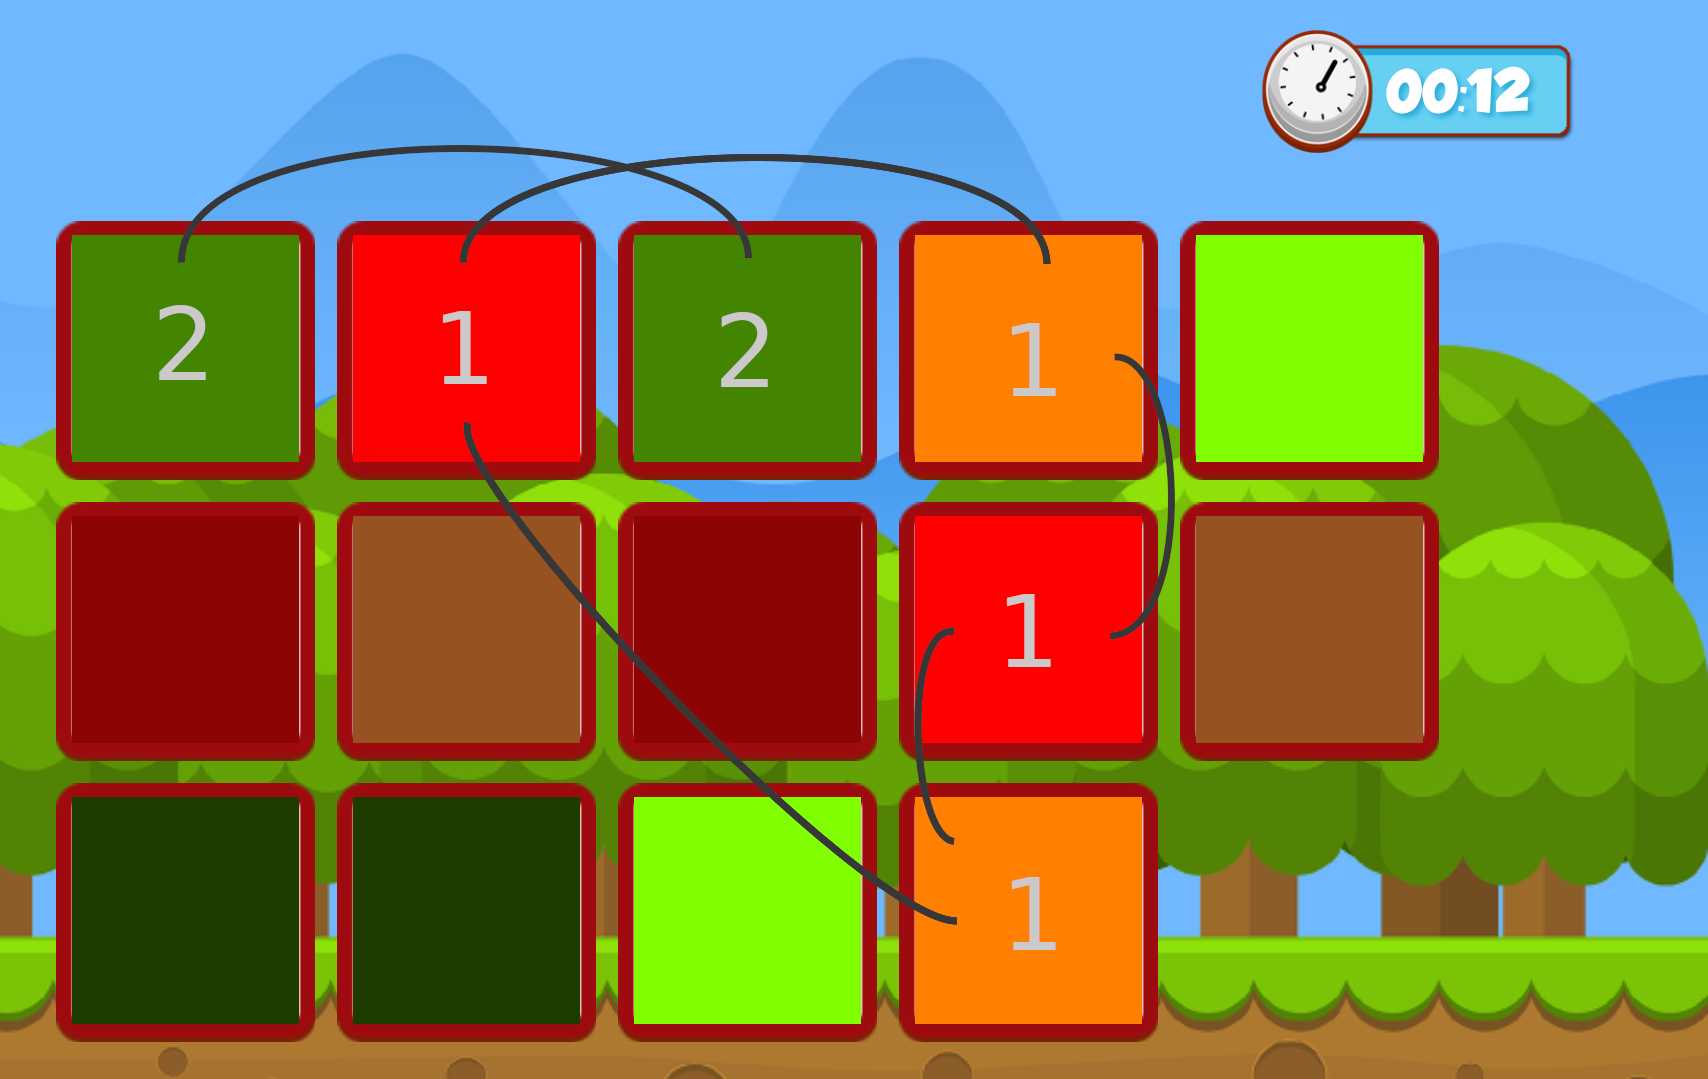
\includegraphics[width=15cm]{images/noObstTurnedNotes.png}
	\caption[Bild kurz]{Examplary showing the number of different comparissons for case 1 and 2. The numbers on the cards represent the case and the edges indicate unique comparissons. All cards are turned face up. A game without any obstacles is used only for the purpose of clarifying the differnet comparissons. All screenshots used for the actual calculation are taken from glare effect games.}
	\label{fig:noObstTurnedNotes}
\end{figure}

First it is calculated how many screenshots are necessary for the first case. For two different coloured arbitrary but fixed cards there can be 
\begin{equation*}
C\textsubscript{1} = 14 \cdot 13 = 182 
\end{equation*}
combinations of positions are possible. The reason that it is not not 14 $\cdot$ 14 is that 14 comparissons of cards with themself would be included. We formulate the condition that enough screenshots need to be taken so that a arbitrary but fixed combination of positions for two different colours is included with a probability of 95\%. 

\begin{center}
	As there are 4 such combinations of positions in each game the probanility P(A) to get a specific combination in a game is 
	\begin{equation*}
		P(A) = \frac{4}{182} % = 0.02198
	\end{equation*}
	The counter probability P($\lnot$A) is 
	\begin{equation*}
		P(\lnot A) = 1 - \frac{4}{182} = \frac{178}{182}%0.02198 = 0.97802
	\end{equation*}
	The number of necceary screenshots to include a specific combination with 95\% probaility is calculated by solving
	\begin{align*}
		1 - P(\lnot A)^n &\geq 0.95 \\
		1 - \left(\frac{178}{182}\right)^n &\geq 0.95 \\
		1 &\geq 0.95 + \left(\frac{178}{182}\right)^n\\
		\left(\frac{178}{182}\right)^n &\leq 0.05\\
		n &\geq log_{(\frac{178}{182})}(0.05) \\
		n &\geq 134.8024 %\llap{$\implies$\hspace{50pt}} at beginnging for implication arrow
	\end{align*}
\end{center}
This means that about 135 Screenshots of games are needed in the first case. Now we perform the same calculation for the second case where there is only one combination of positions for the colours. However, there are less combinations of positions that are relevant than in the first case. For example for two green cards at index 0 and 1 the 182 comparissons would include a comparison of the first green card and the second green card as well as a comparisson of the second green card and the first green card. This goes for every two cards with the same colour, meaning there are only half as many different comparissons in the second case than in the first case. As a result the number of possible combinations in the second case is
\begin{equation*}
C\textsubscript{2} = \frac{C\textsubscript{1}}{2} = \frac{14 \cdot 13}{2} = 91.
\end{equation*}
Now we calculate how many screenshots must be taken to include a specific combination of positions for two equal colours with a probability of 95\%. 
\begin{center}
	As there is one such combinations of positions in each game the probanility P(A) to get a specific combination in a game is 
	\begin{equation*}
		P(A) = \frac{1}{91} % = 0.02198
	\end{equation*}
	The counter probability P($\lnot$A) is 
	\begin{equation*}
		P(\lnot A) = 1 - \frac{1}{91} = \frac{90}{91}.%0.02198 = 0.97802
	\end{equation*}
	The number of necceary screenshots to include a specific combination with 95\% probaility is calculated by solving
	\begin{align*}
		1 - P(\lnot A)^n &\geq 0.95 \\
		1 - \left(\frac{90}{91}\right)^n &\geq 0.95 \\
		1 &\geq 0.95 + \left(\frac{90}{91}\right)^n\\
		\left(\frac{90}{91}\right)^n &\leq 0.05\\
		n &\geq log_{(\frac{90}{91})}(0.05) \\
		n &\geq 271.111 %\llap{$\implies$\hspace{50pt}} at beginnging for implication arrow
	\end{align*}
\end{center}
This means that about 272 screenshots of games are needed in the second case. As there are more screenshots needed for the second case, the first case is also included. This inclusion is caused by the fact that each screenshot includes comparissons for the  fist  as well as the second case. To have a buffer the decision was made to take screenshots of 300 games. In theory these screenshot include any arbitrary but fixed combinations of positions and colours with a probability of over 95\%.\\\\
To assure that these screenshots actually include most of the combinations and therefore eliminate the positional influence of cards, the coverage of combinations can be additionally calculated. Therefore the number of unique combinations included in the 300 screenshots must be divided by the overall number of possible combinations. The number of unique combinations can be counted during the process of creating the similarity matrix, but the number of possible combinations must seperatly determined. The similarity matrix for glare effect has 28 entries, from which 7 are comparissons between same and 21 between different colours. With \textit{C\textsubscript{1}} and \textit{C\textsubscript{2}}  being the possible combinations for two arbitrayry but fixed coloured cards in the two cases mentioned above, the number of overall possible combinations C is
\begin{align*}
C &= 21 \cdot C\textsubscript{1} + 7 \cdot C\textsubscript{2}\\
&= 21 \cdot 182 + 7 \cdot 91\\
&= 4459. 
\end{align*}
Furthermore is was verified that certain combinations are not included significantly more often than others and in that sense have stronger influence on the result. This was not the case ...\todo{code ergänzen und nachprüfen wie oft die combinationen vorkamen..histogramm?}. \\\\
Nonetheless, this does not solve the second problem of extracting single pixels that can potentially be directly in the area of a sunbeam. This can be fixed, by extracting all pixels in a certain are of the card and averaging their rgb values. %By averaging all colours in a certain area, the result will be more representitive of what the player actually sees \todo{Quelle finden wo sowas über visuellen kram gesagt wird}. 
\subsubsection{Implementation}
This section will show and explain the implementation of the similarity matrix generation. Not every line of code will be included, but rather the most important parts. First of all the screenshots and the information about the original colours of the cards are loaded. Before the actual calculation of a similarity matrix for each image, the average rgb values of the cards on the field need to be determined. 
\begin{lstlisting}[language=python, caption=Add caption]
def determine_glare_rgb_values(image):
	'''
	Calculates the rgb average rbg values for each card in an image.
	:param image: The screenshot of the memory game with all cards 
	turned face up.
	:return: The average rbg values in the specified 150 x 150 pixel 
	areas for each card. 
	'''
	glare_rgb_values = []
	for corner in card_corners:
		x_border = corner[0] + 150
		y_border = corner[1] + 150
		card_values = []
		for x in range(corner[0], x_border, 1):
			for y in range(corner[1], y_border, 1):
				coordinates = x, y
				pixel_values = image.getpixel(coordinates)
				card_values.append(pixel_values[:-1])
		card_r = int(round(np.mean([color[0] for color in card_values])))
		card_g = int(round(np.mean([color[1] for color in card_values])))
		card_b = int(round(np.mean([color[2] for color in card_values])))
		glare_rgb_values.append((card_r, card_g, card_b))
	return glare_rgb_values 
\end{lstlisting}
The cards are each 250 $\cdot$ 250 pixels big and the rgb values are extracted from squared 150 $\cdot$ 150 pixel areas. The coordinates the pixels are extracted from are manually selected in gimp. As a result the areas are only correct for the used resolution of 1080p. Once the mean rgb values in those areas are calculated the similarity matrix can be created. Each of the 28 cells in the similarity matrix falls into one of the two cases explained in \todo{ref}, meaning there are either 4 or only 1 unique combination for the calculation of each cell value. For every combination the lab colour distance is determined and the values for each cell are averaged. This completes the steps for a single image, resulting in a similarity matrix with unscaled values. 
%\begin{lstlisting}[language=python, caption=Add caption]
%def determine_distance(color_1_rgb, color_2_rgb):
%	'''
%	Determines dinstance between colors with delta e formula. 
%	:param color_1_rgb: The first color.
%	:param color_2_rgb: The second color.
%	:return: The delta_e distance between the two colours. 
%	'''
%	lab_1 = convert_color(color_1_rgb, LabColor)
%	lab_2 = convert_color(color_2_rgb, LabColor)
%	
%	if cie_1976:
%		detlta_e = delta_e_cie1976(lab_1, lab_2)
%	else:
%		detlta_e = delta_e_cie2000(lab_1, lab_2, Kl=1, Kc=1, Kh=1)
%	return detlta_e
%\end{lstlisting}
Once a similarity matrix for every image is created, the average of all matrices is calculated. During the whole calculation of the single matrices it is being kept track of the highest occurring colour differnece. The last step neccessary to complete the final similarity matrix is to use the highest colour differnce to scale all values down to be between 0 and 1. 

Through the original colours loaded in the beginning, the coverage of combinations in the 300 games can be calculated. 
\begin{lstlisting}[language=python, caption=Add caption]
def determine_coverage(original_colors):
	'''
 	For calculating how many of the combinations are includes 
	in the calcuation. 
	The calculations are based on having 14 cards on the field.
	:param original_colors: A list containing tuples with the card name, 
	the mappimg number for the card, and the index for each card on the 
	screenshot for all screenshots.
	:return: The coverage of combinations of positions 
	for all colour combinations. 
	'''|\Suppressnumber|
	
	[...]|\Reactivatenumber{18}|
	
	combinations = []
	for colors in original_colors:
		for i in range(len(colors)):
			original_color_1 = colors[i]
			for l in range(len(colors)):
				original_color_2 = colors[l]
				if original_color_1[2] != original_color_2[2] and (original_color_2, original_color_1) not in combinations and (original_color_1, original_color_2) not in combinations:
						combinations.append((original_color_1, original_color_2))    
	return len(combinations) / number_of_total_combinations
\end{lstlisting}

\subsubsection{Manual testing}
To verify the correcteness of the color extraction and the calculation of the similarity matrix, the main funtionalities are manually tested. The colour extraction was tested by extracting colours of a screenshot with the skript and compoaring the rgb values to the actual values in the images using gimp. Furthermore the calculation of the delta e score was tested, by comaring results of the script with those of an online calculator. 

\subsection{Screenshot extraction}
To play the memory game and take screenshots an emulator for the pixel 2 in android studio was used. In order to take the screenshots in the needed way and collect additionally necessary information some changes to the memory game were made. In the way the game is intended there are always only maximum two cards turned face up. However, for the screenshots all cards need to be turned around so that the colour differneces can be calculated. Therefore the memory game was adjusted so that all cards are turned face up once the player turns a card. Additionally it was changed so that cards stay face up once they get turned around for the first time. This makes it possible to take screenshots with the colours of all cards visible. Furthermore, for the creation of the similarity matrix it needs to be known what the original colours without the influnece of the simulated sun are. To collect the screenshots and the according colours of the cards in each game a semi-automatic approach was chosen. Once a game is started and a card is flipped, resulting in all cards being turned face up, the colours of all cards are saved in a list. Then a screenshot is manually taken and afterwards the game is exited to enter the main menu. From there on the process is repeated 300 times. As a result there are 300 hundred screenshots of games and a two dimensional list that includes the colours of the cards in the 300 games. The first dimension specifies the game and the second dimension the index of the card. The values of this list are stored in a text file before the game is completely closed. To assure that no mistakes were made when taking the screenshots, the number of collected screenshots is observed during the whole process and afterwards all screenshots are manually checked so that all cards are turned face up. 

\subsection{Final Matrix}
In figure \ref{fig:simMatrix} the final similarity matrix can be seen, dsiplaying how colour differneces are observed under the influence of the simulated sunlight, averaged over 300 games. As mentioned before, the lower the delta e score the more similar the cards appear to the human eye. 
\begin{figure}[H]
	\centering
	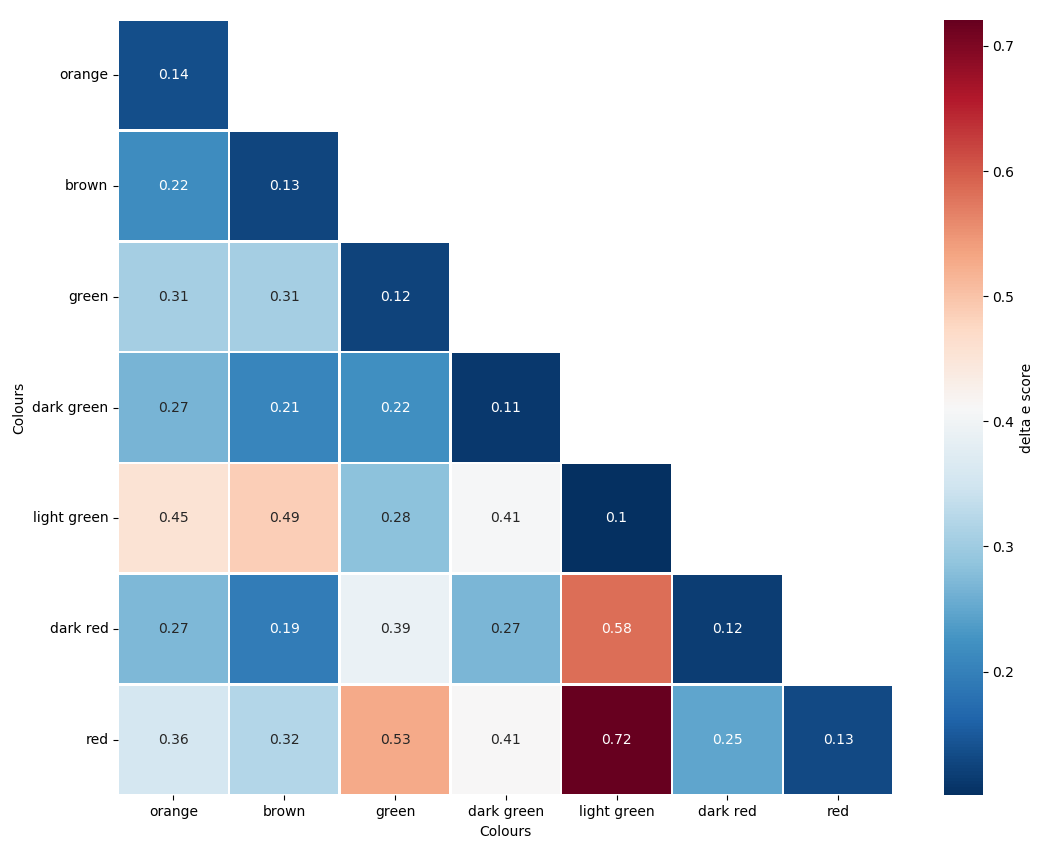
\includegraphics[width=15cm]{images/simMatrix.png}
	\caption[Bild kurz]{Add caption}
	\label{fig:simMatrix}
\end{figure}
The 300 games used for creating this matrix include 99.57\% of all possible combinations. Before actually using the constructed simialry matrix in the simulator it is unknown if the chosen approach results in high quality simulations. If this is not the case it is possible to change the concept or try other approches. 

\subsection{Incorporation of the matrix}


- structure of logs and mapper that maps logs and replaces old matrix with new one\\
- methode für mapping bereits vorhanden, aber es mussten einige anpassungen gemacht werden und ergänzungen: neue matrix einfügen statt der alten, bentzte funktionen wurden nicht mehr unterstützt und mussten geändert werden, methode wurde in ein neues skript eingebaut welches das mapping für alle logs macht und das ergebnis in einer neuen datei speichert.\\
- was ich gemacht habe um zu überprüfen ob mapping nocfh korrekt ist: vergleichen von altem und neuen mapping 

\section{Removing invalid logs}
For the simualation to work, the game log that is used for the simulation must have had all cards turned around at least once. Initially, this was not the case. Therefore a script was written that collects all no obstacle and all glare effect logs, validates them and saves only the valid ones in new files. It need to be noted, that if at least one the two logs from a participant is invalid, both logs are removed. Otherwise the training data could include no obstacle games but no glare effcect logs from a participant and vise versa, which should be avoided \todo{mehr erklären wieso das nicht gut ist und vielleicht quelle finden}. A log is invalid if not all cards were turned at least once. 
\begin{lstlisting}[language=python, caption=Add caption]
def validate_log(log):
	'''
	Validates logs.
	:param log: The log to validate. 
	:return: If the log is valid.
	'''
	needed_entries = ['1.1,', '2.1,', '3.1,', '4.1,', '5.1,', '6.1,', '7.1,', '1.2,', '2.2,', '3.2,', '4.2,', '5.2,', '6.2,', '7.2,']
	for needed_entry in needed_entries:
		if needed_entry not in log:
			return False
	return True
\end{lstlisting}

\section{Simulation}
Multiple additions were made to the simulator. In total four classes were added. Two are for generating configuration files for the simulation of game with and without the glare effect obstacle (NoObst\_ConfigGenerator\_dataCollection2020.java and GlareEffect\_ConfigGenerator\_dataCollection2020.java) and the other two for using those files to simulate new games based on the user behaviour in the original games (NoObstWinStrategyTrainingDataGenerator\_dataCollection2020.java and GlareEffectWinStrategyTrainingDataGenerator\_dataCollection2020.java). These classes utilize the functionalities already implemented in the simulator. \todo{Code grob für jeweils eine zeigen}

\section{Evaluation of simulation}
- intial results\\
- problems\\
- chnages\\
- final results \\
- im realfall benutzen wir nicht alle simulationen sondern nur die besten. die werden vorher nach güte sortiert und dann nur die besten 1-10 und 20 genommen. Bilder zeigen wie es da aussieht bei finalem. \\
- resulkts show that the similarity matrix used creates very good simulations of glare effect games. \\
- t-stochastic test kram (siehe mazens nachricht)



 


%...

%% --------------------
%% |   Appendix part, if needed   |
%% --------------------
\appendix
%\include{anhang_a}
%\include{anhang_b}

%% --------------------
%% |   Bibliography   |
%% --------------------
\cleardoublepage
\phantomsection
\addcontentsline{toc}{chapter}{\bibname}

\bibliographystyle{alpha}
\bibliography{thesis}

% Index
\cleardoublepage
\phantomsection
\printindex
\end{document}
